% !TEX root = main.tex
\chapter{Theory}

\section{Bridge Weigh-in-Motion}
A Bridge Weigh-in-Motion system is based on measurements of a bridge's deformation. The BWIM system uses these measurements to calculate passing vehicles axle loads.
There are different approaches to assembling such a system, but they typically consists of a strain gauge measuring the strain induced by passing vehicles, a axle detector used to find the vehicle speed and spacing of axles and a computer or data storage device. An algorithm then is able to use the data gathered from the axle detector and strain gauge to calculate axle loads \cite{Quilligan}.
\subsection{Moses' Algorithm}
Moses' algorithm is based on the fact that a moving load along a bridge will set up stresses in proportion to the product of the value of the influence line and the axle load magnitude. The influence line being defined as the bending moment at the point of measurement due to a unit axle load crossing the bridge \cite{Quilligan}.

Moses' algorithm is built from the fact that a moving unit load on a bridge will induce stresses proportional to the product of the value of the influence line and the axle load magnitude.

Each individual girder's stress is related to moment:
\begin{equation}
\sigma_{i} = \frac{M_i}{W_i}
\end{equation}
Expressing the moment in terms of strain gives
\begin{equation}
M_{i} = W_{i} \sigma_{i} = E W_{i}  \varepsilon_{i}
\end{equation}
Where:
\begin{description}
	\item $\sigma_{i} = $ the stress in the i'th girder
	\item $ M_i $ = the bendind moment in the i'th girder
	\item $ W_i $ = the section modulus
\end{description}
\begin{description}
	\item E =  The modulus of elasticity
	\item $ \varepsilon_i $ = strain in the i'th girder
\end{description}
The sum of the individual girder moments is therefore:
\begin{equation}
M = \sum_{i = 1}^{N} M_i = \sum_{i = 1}^{N} EW_i \varepsilon_i = EW \sum_{i = 1}^{N} \varepsilon_i
\label{equation:moment_strain}
\end{equation}
The sum of the girder strains is proportional to the gross bending moment. The total bending moment and the measured strain is thus directly related by $EW$. These constants can be calculated through the bridge's dimensions and material properties. However through measuring the effects of a known vehicle passing the bridge these constants can be derived.

Weigh in motion is an inverse type problem, the strain is measured and the cause of the strain is to be calculated. The theoretical bending moment corresponding to axle loads on the bridge at one strain sample, is given by:
\begin{equation}
M_k^T = \sum_{i = 1}^{N} A_i I_{(k-C_i)}
\label{equation:theoretical_strain}
\end{equation}
\begin{equation}
C_i = (L_i \times f)/v
\end{equation}
Where:
\begin{description}
	\item N = \textit{the number of vehicle axles}
	\item $A_i = $ \textit{the weight of axle i}
	\item $I_{k-C_i} = $ \textit{the influence line ordinate for axle i at sample k}
	\item $L_i$ = the distance between axle i and the first axle in meters
	\item $C_i$  = \textit{The number of strain samples corresponding to the axle distance $L_i$}
	\item f = the strain gauge's sampling frequency, in \SI{}{\Hz}
\end{description}

\section{Influence lines}
A influence line can be defined as: "A graph of a response function of a structure as a function of the position of a downward unit load moving across the structure."
For a BWIM system this response function typically is the bending moment at the sensor location.
% "the bending moment, stress, shear or other effect at the point of measurement due to a unit axle load moving along the bridge \cite{bwim_an_overview}".
The influence line could be found through assembling a model of the bridge in any CAD or frame-program, this would however take a lot of time especially for more advanced bridge's. Depending on the support of the bridge the influence lines takes different theoretical forms, as seen in Figure \ref{fig:theoreticalInfl}. The true influence line for a bridge lie somewhere in between the simply supported and fixed version \cite[p.~146]{bwim_an_overview}.
\begin{figure}[h]
\centering
\includegraphics[width=\textwidth]{figures/inflLinesQuilligan}
\caption{Influence lines for simply and fixed supported bridges, figure from \cite{Quilligan}}
\label{fig:theoreticalInfl}
\end{figure}

Znidaric and Baumgärter \cite{bwim_an_overview}, did a study on the effect of choice of influence line. This study shows errors up to 10\% for a short \SI{2}{\metre} bridge span and errors of several hundred percent for a \SI{32}{\metre} bridge span, illustrated by figure \ref{fig:errorOfInfl} showing how a veihicles gross weight is affected when the influence line is varied from a simply supported version to a fixed support version. This underlines the importance of using correct influence lines for a B-WIM system.
\begin{figure}[h]
	\begin{adjustbox}{center}
		\includegraphics[width=1.2\textwidth]{figures/error_in_weights_dueTo_infl}
	\end{adjustbox}
\caption{Errors of axle loads due to wrongly selected influence lines, figure from \cite{Quilligan}}
\label{fig:errorOfInfl}
\end{figure}

\subsection{Using influence lines, in the BWIM system}
Even if a correct influence line for a BWIM setup is found, wrong placement of the influence line with respect to the strain signal is a major source of error. In theory it should be possible to detect the excact point of a axle passing over the sensor, as it results in a peak in the strain signal. This peak corresponds to the major peak in the influence line. A good example of this is seen in figure \ref{fig:strain_vs_influenceLine}, which shows the influence line aligned with the strain signal from a 3 axle vehicle.
\begin{figure}[htbp]
	\begin{adjustbox}{center}
		\includegraphics[width=\textwidth]{figures/strain_vs_influenceline}
	\end{adjustbox}
	\caption{Placement of influence lines, influence line has been scaled.}
	\label{fig:strain_vs_influenceLine}
\end{figure}
The first peak of the strain signal corresponding to the the first axle of the vehicle should occur at the same location as the the peak of the influence line, which should be precisely at the sensor location.
For closely spaced axles it may be difficult to detect the individual peaks, because the both influence the sensor at the same time and because of system noise and dynamics.

\subsection{Influence line through the Matrix Method}
Quilligan \cite{Quilligan} developed a 'matrix method' to calculate the influence line of a bridge through the measured strain induced by a vehicle. This method is derived from Moses', equation \ref{equation:moses}. The matrix method calculates a influence line for a specific strain signal given a known train with known axle weights and velocity. The found influence line is therefore subject to system noise and dynamics which are likely to vary from vehicle to vehicle. An averaging of a sufficient number of calculated influence lines should reduce the dynamic effects. The following description of the matrix method is an extension of Quilligans thesis "Bridge Weigh-in Motion : Development of a 2-D multi-vehicle algorithm \cite{Quilligan}", and shows the math for a general case with unlimited number of vehicle axles.
\begin{equation}
Error = \sum_{k = 1}^{K} [\varepsilon_{k}^{measured} - \varepsilon_{k}^{theoretical}]^2
\label{equation:moses}
\end{equation}
Equation \ref{equation:moses} were originally used to filter out the dynamic response of the bridge.
The theoretical strain in this equation can be expressed as a product of axle loads and influence ordinates at sampling points, see equation \ref{equation:theoretical_strain}, thus we can expand equation \ref{equation:moses}:
\begin{equation}
Error = \sum_{k = 1}^{K} \Big[\varepsilon_{k}^{measured} - \Big(\sum_{i = 1}^{N} A_i I_{(k-C_i)}\Big)\Big]^2
\label{equation:moses_expanded}
\end{equation}
The set of influence ordinates $I$ that minimizes $Error$, forms the wanted influence line.
\begin{equation}
\frac{\partial Error}{\partial I_R} = \frac{\partial \sum_{k = 1}^{K} \Big[\varepsilon_{k}^{measured} - \Big(\sum_{i = 1}^{N} A_i I_{(k-C_i)}\Big)\Big]^2}{\partial I_R}
\end{equation}
For a given number of known axle loads this equation comes down to a set of $(K - C_n)$ number of linear equations. Rearranging the equations and writing them in matrix form leads to:
\begin{equation}
\begin{bmatrix} Am \end{bmatrix}_{K-C_N, K-C_N} \begin{Bmatrix} I \end{Bmatrix}_{K-C_N, 1} = \begin{Bmatrix} M \end{Bmatrix}_{K-C_N, 1}
\label{equation:matrixForm}
\end{equation}
Where:
\begin{description}
\item $\begin{Bmatrix} M \end{Bmatrix}$ = a vector depending on axle weights and measured strain, $M_{i, 1} = \Big(\sum_{j = 1}^{N} A_j \varepsilon_{(i+C_j)}\Big)$
\item $\begin{bmatrix} Am \end{bmatrix}$ is a matrix depending only on the axle loads, defined by equation \ref{axleMatrix}.
\end{description}
\begin{equation}
\begin{bmatrix} Am \end{bmatrix} = \sum_{i = 1}^{N} \sum_{j = i}^{N} \begin{bmatrix} Am \end{bmatrix} + \big( A_i A_j  \begin{bmatrix} D \end{bmatrix}_{C_j - C_i}\big)
\label{axleMatrix}
\end{equation}
Which produces the upper triangle of the symmetric $ \begin{bmatrix} Am \end{bmatrix} $ which through the transpose operation can be used to build the full matrix.
Where:
\begin{description}
\item $\begin{bmatrix} D \end{bmatrix}_{C_j - C_i}$ = a matrix containing only one diagonal of ones, where the diagonal is placed with an offset, $C_j - C_i$, from the center matrix diagonal.
\end{description}
Solving equation \ref{equation:matrixForm} for the influence ordinate vector gives the influence line for the strain history. This can be done through inversion of the $\begin{Bmatrix} M \end{Bmatrix}$ (equation \ref{axleMatrix}) or other numerical solutions like a Cholesky factorization. In this project this was done through Matlab's \textbackslash operator.
When the influence line and the axle spacings are known, the axle weights can be calculated by solving
\begin{equation}
	A = \begin{Bmatrix} I \end{Bmatrix} \textbackslash \epsilon
\end{equation}
\subsection{Influence line through Optimization}
testing \cite{Liljencrantz}.
For this thesis one of the goals where to assess the accuracy of and optimization algorith for finding a bridges influence lines. To develope such an algorithm test strain signal where produced by a matlab script, and the algorithm developed was to find the influence line used to produce the strain signal.
In theory using optimization to identify influence lines should work well, and indeed it did for these produced theoretical strain signals.

The method of optimization developed for this project, utilized matlabs "fmincon" function which finds the minimum value of a constrained function. The function chosen to minimize was Moses' equation \ref{equation:moses_expanded}.
\begin{easylist}[enumerate]
	& create initial guess of influence line
	& use initial guess values as input to fmincon
	& for each iteration of fmincon, a new influence line is built from the optimized values
	& The found influence line forms a influence ordinate matrix, based on known axle spacings
	& equation \ref{equation:moses_expanded}, is calculated resulting in an error value
	& steps 3 - 5 is repeated until either function tolerance is reached, or other tolerance values is exceeded.
\end{easylist}
\section{Finding the train's speed}
\label{section:trainSpeed}

\begin{easylist}[itemize]
 & By identifying a peak representing the same axle in the strain signals for two different sensors. The time difference between two such peaks is the time the train uses to travel the distance between the two sensors. Given the known distance between the sensors, s, the velocity is given by $v = s/t$.
 & Through doing cross correlation between two sensors strain signals. Cross correlation measures the similarity between two signals as a function of the lag. This can be used to identify the lag between two similar signals. The cross correlation of two signals has maximum value at the lag equal to the delay. The time delay is then a product of the sampling frequency and the lag in samples.
\end{easylist}

\section{The axle distances}
Identifying axles in the strain signal is done through identifying standalone peaks, however due to system noise and dynamic effect finding excact positions of axles in the signal
\section{Filtering and noise}
All signals are subjected to noise, which can be defined as
\begin{displayquote}
	unwanted disturbances superposed upon a useful signal that tend to obscure its information content \cite{IEEE_electronics}
\end{displayquote}
Noise in a BWIM system can be intrinsic noise, that is noise generated inside a system, and extrinsic noise which is noise generated outside the system. A train approaching the BWIM sensors may be a source of extrinsic noise.
Performing bridge weigh-in motion relies upon the information provided by the sensor signals. When the distances between axles is to be found, noise is a source of distortion which may increase error of found distance, it may also make it difficult for the program to detect the desired peaks in the signal which corresponds to the trains axles. Smoothing the signal may therefore completely necessary for a BWIM system. During the developement of the software for this thesis, several attempts on finding and using appropriate filters have been made. Matlab contains many such filter functions which can be used, such as a Butterworth and SGOLAY filters.
\subsection{Noise smoothing through fourier transformation}
The following quotation from  Matlabs: Practical Introduction to Frequency-Domain Analysis, see \cite{frequency_domain_analysis}, describes how frequency analysis can be done with Matlab.
\begin{displayquote}
	Frequency-domain analysis shows how a signal's energy is distributed over a range of frequencies. A signal can be converted between the time and frequency domains with a pair of mathematical operators called a transform. An example of this is the Fourier transorm which decoposes a function into the sim of a number of sine wave frequency components. The 'spectrum' of frequency components is the frequency domain representation of the signal. The inverse Fourier transform converts the frequency domain function back to a time function.
\end{displayquote}

Performing a fast fourier transformation in matlab on a vector signal, gives the oportunity to remove unwanted frequencies from the signal. When the signal is transformed into the frequency domain, setting all the frequencies above 30 Hz to zero and then transforming the signal back into the time domain would smooth a typical BWIM signal greatly.
Figure \ref{} shows filtering of a strain signal where frequencies above 20 Hz have been eliminated.
\begin{figure}[htpb]
	\begin{subfigure}[t]{0.9\textwidth}
		\centering
		% This file was created by matlab2tikz.
%
%The latest updates can be retrieved from
%  http://www.mathworks.com/matlabcentral/fileexchange/22022-matlab2tikz-matlab2tikz
%where you can also make suggestions and rate matlab2tikz.
%
\definecolor{mycolor1}{rgb}{0.00000,0.44700,0.74100}%
%
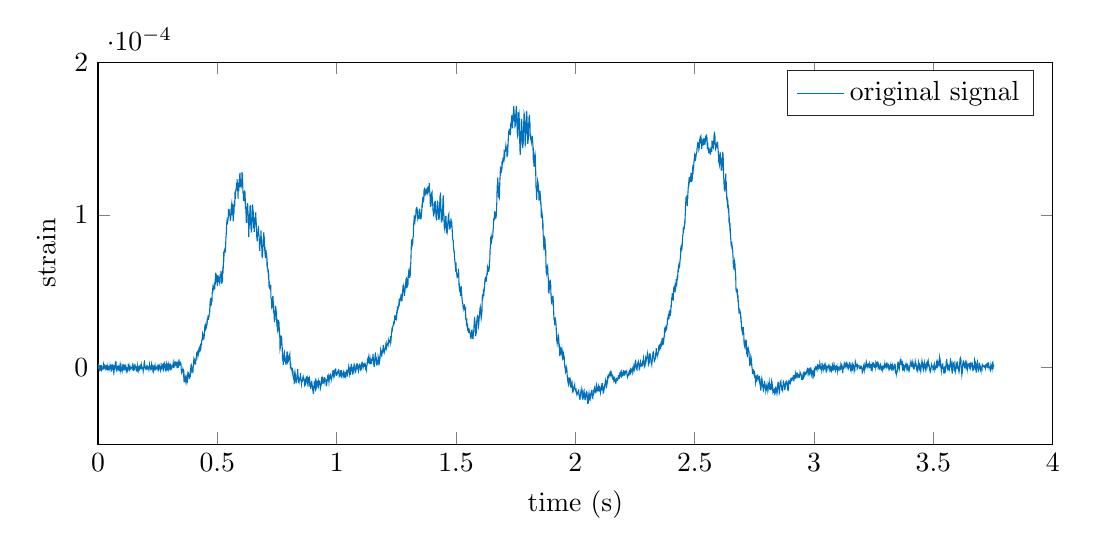
\begin{tikzpicture}

\begin{axis}[%
  width=\textwidth,
  height=0.4\textwidth,
  at={(0\figurewidth,0\figureheight)},
scale only axis,
xmin=0,
xmax=4,
xlabel={time (s)},
ymin=-5e-05,
ymax=0.0002,
ylabel={strain},
axis background/.style={fill=white},
legend style={legend cell align=left,align=left,draw=white!15!black}
]
\addplot [color=mycolor1,solid]
  table[row sep=crcr]{%
0	-5.3402874771488e-07\\
0.0009765625	-3.43481049059832e-07\\
0.001953125	1.12444437659794e-06\\
0.0029296875	1.57589168782316e-07\\
0.00390625	5.88086514129562e-07\\
0.0048828125	-9.15123929029135e-07\\
0.005859375	-1.58556845641423e-06\\
0.0068359375	-1.2538749595344e-06\\
0.0078125	-8.65722718068184e-07\\
0.0087890625	1.55494254731881e-06\\
0.009765625	1.64425781753151e-08\\
0.0107421875	1.64646499349478e-07\\
0.01171875	1.66080280952926e-06\\
0.0126953125	-2.09369424129715e-06\\
0.013671875	-2.87022457852925e-07\\
0.0146484375	1.57589168782316e-07\\
0.015625	-1.38090653730816e-06\\
0.0166015625	-9.7158244991534e-07\\
0.017578125	4.96341147421513e-07\\
0.0185546875	3.55194462001249e-07\\
0.01953125	-1.28916151212574e-06\\
0.0205078125	1.2230251742666e-07\\
0.021484375	1.15245187452123e-07\\
0.0224609375	5.31627824949159e-07\\
0.0234375	1.78077780023204e-06\\
0.0244140625	5.88086514129562e-07\\
0.025390625	9.05666758545124e-07\\
0.0263671875	-2.1644920995649e-07\\
0.02734375	1.2230251742666e-07\\
0.0283203125	9.97412199721381e-07\\
0.029296875	5.527998326513e-07\\
0.0302734375	1.08187857575815e-07\\
0.03125	3.55194462001249e-07\\
0.0322265625	-3.15251754246437e-07\\
0.033203125	1.20207516710871e-06\\
0.0341796875	1.32910739553994e-06\\
0.03515625	8.42150693662223e-07\\
0.0361328125	-1.04215559213437e-06\\
0.037109375	-1.03509827835717e-06\\
0.0380859375	-2.09391884623857e-07\\
0.0390625	9.05666758545124e-07\\
0.0400390625	-9.64746658658512e-08\\
0.041015625	-7.52805646271181e-07\\
0.0419921875	1.39968086960681e-06\\
0.04296875	-2.30563860325987e-07\\
0.0439453125	-1.38818625863065e-07\\
0.044921875	1.32910739553994e-06\\
0.0458984375	-6.75175144744305e-07\\
0.046875	-3.71710342292678e-07\\
0.0478515625	-6.68117825831016e-07\\
0.048828125	-2.87022457852925e-07\\
0.0498046875	-9.50410505323523e-07\\
0.05078125	9.19781440716656e-07\\
0.0517578125	3.05572354581188e-08\\
0.052734375	1.08187857575815e-07\\
0.0537109375	-1.52933278405303e-07\\
0.0546875	7.29233264734229e-07\\
0.0556640625	2.2816247890003e-07\\
0.056640625	-8.37493452489216e-07\\
0.0576171875	-1.5999060452832e-07\\
0.05859375	2.20421917203491e-06\\
0.0595703125	-1.11272872447784e-06\\
0.060546875	-7.73977599159096e-07\\
0.0615234375	-8.37493452489216e-07\\
0.0625	-4.21111601647426e-07\\
0.0634765625	7.71577297619319e-07\\
0.064453125	3.05793131436969e-07\\
0.0654296875	-1.70554264623899e-06\\
0.06640625	-6.75175144744305e-07\\
0.0673828125	-2.07957964307496e-06\\
0.068359375	-7.03404419409538e-07\\
0.0693359375	-4.9168482090271e-07\\
0.0703125	6.0220118741237e-07\\
0.0712890625	1.54082784736939e-06\\
0.072265625	-2.58793159879731e-07\\
0.0732421875	1.71020427283263e-06\\
0.07421875	2.43711207808129e-06\\
0.0751953125	8.70380054844837e-07\\
0.076171875	1.54788519729477e-06\\
0.0771484375	-1.13390066225458e-06\\
0.078125	-1.6702561227832e-06\\
0.0791015625	-1.10567141168791e-06\\
0.080078125	9.40953464714355e-07\\
0.0810546875	-4.98742142284511e-07\\
0.08203125	1.57589168782316e-07\\
0.0830078125	-3.15251754246437e-07\\
0.083984375	2.77563801859065e-07\\
0.0849609375	1.00446954204195e-06\\
0.0859375	1.13855906489282e-06\\
0.0869140625	-1.52205269730453e-06\\
0.087890625	5.81029177636368e-07\\
0.0888671875	-1.6702561227832e-06\\
0.08984375	-1.50793808308255e-06\\
0.0908203125	-1.57851115024183e-06\\
0.091796875	1.0113052779882e-07\\
0.0927734375	-1.07744215954047e-06\\
0.09375	1.03269891231082e-06\\
0.0947265625	1.8160645676355e-06\\
0.095703125	-2.1644920995649e-07\\
0.0966796875	4.96341147421513e-07\\
0.09765625	-1.11272872447784e-06\\
0.0986328125	-5.90487311267259e-07\\
0.099609375	-9.22181244485338e-07\\
0.1005859375	-1.08449947272549e-06\\
0.1015625	-1.74082916722627e-06\\
0.1025390625	1.08187857575815e-07\\
0.103515625	7.50405280732468e-07\\
0.1044921875	2.57120198186725e-06\\
0.10546875	1.4347450794398e-07\\
0.1064453125	5.17513153641767e-07\\
0.107421875	-1.69848534174537e-06\\
0.1083984375	5.31627824949159e-07\\
0.109375	9.19781440716656e-07\\
0.1103515625	-3.9288231117973e-07\\
0.111328125	-6.04601951167483e-07\\
0.1123046875	-3.29587192037049e-08\\
0.11328125	-1.09861409879931e-06\\
0.1142578125	-8.58665401821382e-07\\
0.115234375	-2.0233455919191e-07\\
0.1162109375	1.11032968869813e-06\\
0.1171875	6.93946573379319e-07\\
0.1181640625	-9.64525135149991e-07\\
0.119140625	9.40731981202703e-08\\
0.1201171875	-4.00160470059342e-08\\
0.12109375	-9.57467820286413e-07\\
0.1220703125	1.99933153667824e-07\\
0.123046875	-2.0090066460384e-06\\
0.1240234375	-1.48676616100896e-06\\
0.125	-4.84627499421379e-07\\
0.1259765625	3.69309128765401e-07\\
0.126953125	2.53591516162456e-06\\
0.1279296875	1.0609282841596e-06\\
0.12890625	2.35219810455116e-07\\
0.1298828125	1.07504297067683e-06\\
0.130859375	-4.28168924017369e-07\\
0.1318359375	5.73971841241836e-07\\
0.1328125	-1.88440633034758e-08\\
0.1337890625	-8.0220686829338e-07\\
0.134765625	-2.09391884623857e-07\\
0.1357421875	-4.06996956610903e-07\\
0.13671875	1.85818491644238e-07\\
0.1376953125	-3.9288231117973e-07\\
0.138671875	-1.95277233661735e-07\\
0.1396484375	7.99585390595919e-08\\
0.140625	1.57589168782316e-07\\
0.1416015625	-1.45875952183624e-07\\
0.142578125	-5.55200709787939e-07\\
0.1435546875	2.84621134105656e-07\\
0.14453125	1.39262352175573e-06\\
0.1455078125	6.23373198076985e-07\\
0.146484375	1.14561640918837e-06\\
0.1474609375	-2.94079782099622e-07\\
0.1484375	-1.98077744445837e-06\\
0.1494140625	-3.29587192037049e-08\\
0.150390625	6.58438803937799e-08\\
0.1513671875	-3.36423725504423e-07\\
0.15234375	9.33896123282837e-07\\
0.1533203125	3.4813712876695e-07\\
0.154296875	1.42085291375267e-06\\
0.1552734375	1.6537454580242e-06\\
0.15625	7.08061249625035e-07\\
0.1572265625	6.37487872347286e-07\\
0.158203125	6.72774559751796e-07\\
0.1591796875	-1.20447378175849e-06\\
0.16015625	-1.60674037433988e-06\\
0.1611328125	-7.95149551158182e-07\\
0.162109375	3.83423795924636e-07\\
0.1630859375	4.4693980303062e-07\\
0.1640625	-4.77570177841603e-07\\
0.1650390625	1.24441923969707e-06\\
0.166015625	1.08187857575815e-07\\
0.1669921875	-3.85824988316259e-07\\
0.16796875	2.32792128737787e-09\\
0.1689453125	-1.48676616100896e-06\\
0.169921875	-5.69315350676088e-07\\
0.1708984375	-7.31633692494437e-07\\
0.171875	-2.17838182233442e-06\\
0.1728515625	-1.38818625863065e-07\\
0.173828125	9.97412199721381e-07\\
0.1748046875	1.08915765758893e-06\\
0.17578125	2.2816247890003e-07\\
0.1767578125	8.20978673812247e-07\\
0.177734375	-3.29587192037049e-08\\
0.1787109375	-3.71710342292678e-07\\
0.1796875	-1.17646646308981e-07\\
0.1806640625	3.4813712876695e-07\\
0.181640625	1.63963075530964e-06\\
0.1826171875	3.55194462001249e-07\\
0.18359375	-2.79965133508e-07\\
0.1845703125	9.40731981202703e-08\\
0.185546875	-1.67047930552241e-07\\
0.1865234375	1.64425781753151e-08\\
0.1875	-5.55200709787939e-07\\
0.1884765625	-8.72780034216324e-07\\
0.189453125	-2.16426722648251e-06\\
0.1904296875	-9.43353190262187e-07\\
0.19140625	-7.81034916590932e-07\\
0.1923828125	2.0842440805924e-06\\
0.193359375	2.87466873787881e-06\\
0.1943359375	1.70314692063563e-06\\
0.1953125	1.4347450794398e-07\\
0.1962890625	1.73843368260723e-06\\
0.197265625	6.58659884493788e-07\\
0.1982421875	-1.24703972925744e-07\\
0.19921875	-7.95149551158182e-07\\
0.2001953125	-9.99811707988159e-07\\
0.201171875	-1.16212991124113e-06\\
0.2021484375	-5.90487311267259e-07\\
0.203125	4.32825134093727e-07\\
0.2041015625	2.32792128737787e-09\\
0.205078125	2.21105147444039e-07\\
0.2060546875	5.88086514129562e-07\\
0.20703125	8.7743739538731e-07\\
0.2080078125	-3.29587192037049e-08\\
0.208984375	5.59857168749194e-07\\
0.2099609375	3.41079795631964e-07\\
0.2109375	2.06990484827828e-07\\
0.2119140625	-4.21111601647426e-07\\
0.212890625	-1.19741647025226e-06\\
0.2138671875	7.29012096774631e-08\\
0.21484375	7.15118587895887e-07\\
0.2158203125	2.13364558537669e-06\\
0.216796875	1.22324720295847e-06\\
0.2177734375	1.23736189401873e-06\\
0.21875	6.72774559751796e-07\\
0.2197265625	-6.61060506819064e-07\\
0.220703125	-1.28916151212574e-06\\
0.2216796875	-1.35267730056832e-06\\
0.22265625	-1.01392633643205e-06\\
0.2236328125	-7.17519056149529e-07\\
0.224609375	1.91486752950049e-06\\
0.2255859375	1.08915765758893e-06\\
0.2265625	1.42791026199905e-06\\
0.2275390625	6.51602547012669e-07\\
0.228515625	2.91678466450476e-07\\
0.2294921875	-1.03509827835717e-06\\
0.23046875	-2.58793159879731e-07\\
0.2314453125	-1.35267730056832e-06\\
0.232421875	-2.13603803359366e-06\\
0.2333984375	-8.72780034216324e-07\\
0.234375	-8.23600117434969e-08\\
0.2353515625	-1.29621882234763e-06\\
0.236328125	1.11738703259859e-06\\
0.2373046875	1.00446954204195e-06\\
0.23828125	3.05572354581188e-08\\
0.2392578125	9.90354857500131e-07\\
0.240234375	-5.55200709787939e-07\\
0.2412109375	-1.38818625863065e-07\\
0.2421875	-6.11659270969818e-07\\
0.2431640625	-2.44678510300401e-07\\
0.244140625	-3.99939633944973e-07\\
0.2451171875	5.87865512094096e-08\\
0.24609375	-4.56398212509432e-07\\
0.2470703125	-2.51735835139506e-07\\
0.248046875	-3.29366401850568e-07\\
0.2490234375	3.69309128765401e-07\\
0.25	-1.10589319593339e-07\\
0.2509765625	-9.36295875101755e-07\\
0.251953125	8.20978673812247e-07\\
0.2529296875	1.15245187452123e-07\\
0.25390625	1.50554109922527e-06\\
0.2548828125	1.54788519729477e-06\\
0.255859375	-1.31761299443844e-07\\
0.2568359375	4.82226477101612e-07\\
0.2578125	2.63449137662955e-07\\
0.2587890625	-8.94173388542221e-08\\
0.259765625	8.49208033809612e-07\\
0.2607421875	-8.37493452489216e-07\\
0.26171875	-1.51499539024287e-06\\
0.2626953125	-7.53026845338924e-08\\
0.263671875	1.03975625512448e-06\\
0.2646484375	-1.38090653730816e-06\\
0.265625	4.68111807176794e-07\\
0.2666015625	3.90481129652464e-07\\
0.267578125	1.8160645676355e-06\\
0.2685546875	1.41379556560539e-06\\
0.26953125	1.55494254731881e-06\\
0.2705078125	3.05572354581188e-08\\
0.271484375	-5.12856784752993e-07\\
0.2724609375	8.06863994406298e-07\\
0.2734375	-4.84627499421379e-07\\
0.2744140625	-1.24681764871988e-06\\
0.275390625	-5.26971426826608e-07\\
0.2763671875	1.87252340061667e-06\\
0.27734375	1.60434400025156e-06\\
0.2783203125	2.54297252547586e-06\\
0.279296875	1.78783515351541e-06\\
0.2802734375	9.19781440716656e-07\\
0.28125	1.16678844266764e-06\\
0.2822265625	-5.90487311267259e-07\\
0.283203125	1.71703830015519e-07\\
0.2841796875	-9.64746658658512e-08\\
0.28515625	-7.81034916590932e-07\\
0.2861328125	6.86889235404888e-07\\
0.287109375	2.60648880457868e-06\\
0.2880859375	1.98544108554236e-06\\
0.2890625	7.645199585583e-07\\
0.2900390625	1.82312192141239e-06\\
0.291015625	1.40673821755655e-06\\
0.2919921875	1.36417177672588e-07\\
0.29296875	1.07504297067683e-06\\
0.2939453125	1.91486752950049e-06\\
0.294921875	2.06990484827828e-07\\
0.2958984375	1.32205004867679e-06\\
0.296875	4.75169142090089e-07\\
0.2978515625	2.55002988942517e-06\\
0.298828125	7.08061249625035e-07\\
0.2998046875	2.56391805712785e-07\\
0.30078125	1.03269891231082e-06\\
0.3017578125	3.05793131436969e-07\\
0.302734375	1.09621500119341e-06\\
0.3037109375	1.58317194840201e-06\\
0.3046875	5.95143850721635e-07\\
0.3056640625	-1.64202690224003e-06\\
0.306640625	1.07504297067683e-06\\
0.3076171875	-8.0220686829338e-07\\
0.30859375	4.75169142090089e-07\\
0.3095703125	7.22175926265835e-07\\
0.310546875	1.67491751283644e-06\\
0.3115234375	1.71020427283263e-06\\
0.3125	1.5619998974415e-06\\
0.3134765625	1.09621500119341e-06\\
0.314453125	2.20421917203491e-06\\
0.3154296875	9.40731981202703e-08\\
0.31640625	1.67491751283644e-06\\
0.3173828125	1.61845870197842e-06\\
0.318359375	-8.23600117434969e-08\\
0.3193359375	2.28185012876646e-06\\
0.3203125	1.39262352175573e-06\\
0.3212890625	1.5619998974415e-06\\
0.322265625	1.66786016113363e-06\\
0.3232421875	3.89798821478094e-06\\
0.32421875	2.44416944054958e-06\\
0.3251953125	2.76880822085504e-06\\
0.326171875	2.93112768937759e-06\\
0.3271484375	2.03484258064733e-06\\
0.328125	3.18519304934469e-06\\
0.3291015625	2.86055400099171e-06\\
0.330078125	2.94524242823988e-06\\
0.3310546875	3.0863898385922e-06\\
0.33203125	1.60434400025156e-06\\
0.3330078125	2.41593999126904e-06\\
0.333984375	1.41379556560539e-06\\
0.3349609375	-4.00160470059342e-08\\
0.3359375	1.85840869177875e-06\\
0.3369140625	1.51965579818676e-06\\
0.337890625	2.88172610647024e-06\\
0.3388671875	1.61140135106555e-06\\
0.33984375	1.9642690176928e-06\\
0.3408203125	3.06521772452093e-06\\
0.341796875	1.70314692063563e-06\\
0.3427734375	3.50983230668457e-06\\
0.34375	3.4392585373114e-06\\
0.3447265625	1.35027943672333e-06\\
0.345703125	3.93327513033151e-06\\
0.3466796875	1.39262352175573e-06\\
0.34765625	2.6629477260533e-06\\
0.3486328125	-1.24681764871988e-06\\
0.349609375	-1.2538749595344e-06\\
0.3505859375	-2.90528297464316e-06\\
0.3515625	-2.23484020179143e-06\\
0.3525390625	-2.0090066460384e-06\\
0.353515625	-1.60674037433988e-06\\
0.3544921875	-1.9384336391252e-06\\
0.35546875	-1.08449947272549e-06\\
0.3564453125	-2.07252234381587e-06\\
0.357421875	-9.0806661347362e-07\\
0.3583984375	-3.25108995115103e-06\\
0.359375	-5.93285029023422e-06\\
0.3603515625	-5.02246482667426e-06\\
0.361328125	-9.41206021390188e-06\\
0.3623046875	-7.66187242104118e-06\\
0.36328125	-8.09941993871566e-06\\
0.3642578125	-8.13470601230821e-06\\
0.365234375	-7.23138175088862e-06\\
0.3662109375	-8.5581387028323e-06\\
0.3671875	-7.68304408386251e-06\\
0.3681640625	-6.93497812503051e-06\\
0.369140625	-9.03802865561635e-06\\
0.3701171875	-7.42898407134055e-06\\
0.37109375	-8.33936519045514e-06\\
0.3720703125	-9.28503065917912e-06\\
0.373046875	-7.61952909273137e-06\\
0.3740234375	-6.34217035066511e-06\\
0.375	-7.11140887569477e-06\\
0.3759765625	-4.16147861254882e-06\\
0.376953125	-3.19463168546932e-06\\
0.3779296875	-3.53338118474719e-06\\
0.37890625	-4.18970769205766e-06\\
0.3798828125	-3.92153137292292e-06\\
0.380859375	-5.60821690261874e-06\\
0.3818359375	-6.28571243104794e-06\\
0.3828125	-7.09729441791319e-06\\
0.3837890625	-7.17492393082332e-06\\
0.384765625	-6.52565854576855e-06\\
0.3857421875	-4.82486156324008e-06\\
0.38671875	-5.0295220846504e-06\\
0.3876953125	-2.4042153022371e-06\\
0.388671875	-5.3402874771488e-07\\
0.3896484375	1.51259844865647e-06\\
0.390625	1.80900721395705e-06\\
0.3916015625	7.08061249625035e-07\\
0.392578125	-7.95149551158182e-07\\
0.3935546875	-1.80434489878119e-06\\
0.39453125	-2.95468398580517e-06\\
0.3955078125	-2.70767888160047e-06\\
0.396484375	-2.47478824396612e-06\\
0.3974609375	4.11653131428573e-07\\
0.3984375	-6.18716590672841e-07\\
0.3994140625	1.95015430628684e-06\\
0.400390625	2.24656332877059e-06\\
0.4013671875	4.75898965910781e-06\\
0.40234375	3.91916036381491e-06\\
0.4033203125	5.17537613085395e-06\\
0.404296875	4.73781747481472e-06\\
0.4052734375	4.15205406185774e-06\\
0.40625	4.74487486948035e-06\\
0.4072265625	4.1591114483255e-06\\
0.408203125	2.03484258064733e-06\\
0.4091796875	4.09559497366796e-06\\
0.41015625	4.7025305029676e-06\\
0.4111328125	5.61293516654782e-06\\
0.412109375	7.05264822177033e-06\\
0.4130859375	8.95815711490756e-06\\
0.4140625	8.70408884648464e-06\\
0.4150390625	7.85719554286424e-06\\
0.416015625	9.98854640461432e-06\\
0.4169921875	1.10895126297611e-05\\
0.41796875	8.09714850116025e-06\\
0.4189453125	9.12047857563533e-06\\
0.419921875	8.6688015971054e-06\\
0.4208984375	1.01296957863354e-05\\
0.421875	1.1054225213465e-05\\
0.4228515625	1.21551937651745e-05\\
0.423828125	1.30091517970177e-05\\
0.4248046875	1.30867844170724e-05\\
0.42578125	1.2162251263644e-05\\
0.4267578125	1.37643059720956e-05\\
0.427734375	1.36584431691216e-05\\
0.4287109375	1.44418284373658e-05\\
0.4296875	1.39266289798177e-05\\
0.4306640625	1.26915639303319e-05\\
0.431640625	1.35666954245203e-05\\
0.4326171875	1.53522506834479e-05\\
0.43359375	1.53099054262544e-05\\
0.4345703125	1.76318422769664e-05\\
0.435546875	1.78365119953624e-05\\
0.4365234375	1.94597575313841e-05\\
0.4375	2.03207855451876e-05\\
0.4384765625	2.22404598520676e-05\\
0.439453125	2.15629269093454e-05\\
0.4404296875	1.81188151915201e-05\\
0.44140625	1.93468359336979e-05\\
0.4423828125	1.97067736144754e-05\\
0.443359375	2.05748596662279e-05\\
0.4443359375	2.00384811163844e-05\\
0.4453125	2.10971235392499e-05\\
0.4462890625	2.31085502652227e-05\\
0.447265625	2.60515996158195e-05\\
0.4482421875	2.54658114455515e-05\\
0.44921875	2.68067733212639e-05\\
0.4501953125	2.76042944435337e-05\\
0.451171875	2.67009077803853e-05\\
0.4521484375	2.55293306118463e-05\\
0.453125	2.58751573242498e-05\\
0.4541015625	2.63833112910921e-05\\
0.455078125	2.73855053375489e-05\\
0.4560546875	2.90017238758656e-05\\
0.45703125	2.79289494208887e-05\\
0.4580078125	3.12954927021653e-05\\
0.458984375	3.20930209230322e-05\\
0.4599609375	3.22906387302611e-05\\
0.4609375	3.38927573833388e-05\\
0.4619140625	3.39351042009215e-05\\
0.462890625	3.13237237680969e-05\\
0.4638671875	3.25164877476311e-05\\
0.46484375	3.3081110733562e-05\\
0.4658203125	3.51772790986389e-05\\
0.466796875	3.52831464189159e-05\\
0.4677734375	3.54101872325843e-05\\
0.46875	4.04918460218449e-05\\
0.4697265625	4.23198441369173e-05\\
0.470703125	4.13105625050984e-05\\
0.4716796875	4.2496292182078e-05\\
0.47265625	4.55453241529184e-05\\
0.4736328125	4.0618888147643e-05\\
0.474609375	4.4041979696804e-05\\
0.4755859375	4.34279388840521e-05\\
0.4765625	4.56088458483342e-05\\
0.4775390625	4.33150119194205e-05\\
0.478515625	4.96883670442277e-05\\
0.4794921875	4.85237944790895e-05\\
0.48046875	5.09305807445248e-05\\
0.4814453125	5.31256362976036e-05\\
0.482421875	5.28009650992676e-05\\
0.4833984375	5.31679847301876e-05\\
0.484375	5.32103331663274e-05\\
0.4853515625	5.22504361537004e-05\\
0.486328125	5.3549120783465e-05\\
0.4873046875	5.27868489649508e-05\\
0.48828125	5.25186424880071e-05\\
0.4892578125	5.12481926931653e-05\\
0.490234375	5.57724201684315e-05\\
0.4912109375	5.7353439027581e-05\\
0.4921875	5.67958469891681e-05\\
0.4931640625	6.21882819176267e-05\\
0.494140625	5.79392642383722e-05\\
0.4951171875	5.59065242542874e-05\\
0.49609375	5.76075318065243e-05\\
0.4970703125	5.84615668073546e-05\\
0.498046875	5.61747325329791e-05\\
0.4990234375	5.87650671972746e-05\\
0.5	5.35420627057869e-05\\
0.5009765625	5.55465607360152e-05\\
0.501953125	5.60547446011952e-05\\
0.5029296875	6.06072479014609e-05\\
0.50390625	5.75016597997398e-05\\
0.5048828125	5.96755694629149e-05\\
0.505859375	5.83768690567189e-05\\
0.5068359375	5.60265121508068e-05\\
0.5078125	5.82992294644656e-05\\
0.5087890625	5.66052776996731e-05\\
0.509765625	5.57371296254485e-05\\
0.5107421875	5.82498224574364e-05\\
0.51171875	6.01061176183312e-05\\
0.5126953125	6.12848333014719e-05\\
0.513671875	5.88074161034121e-05\\
0.5146484375	6.07484114513888e-05\\
0.515625	6.3367002467272e-05\\
0.5166015625	5.95908715083943e-05\\
0.517578125	5.51019002740457e-05\\
0.5185546875	6.22941549082762e-05\\
0.51953125	5.51865974746705e-05\\
0.5205078125	5.76639968858971e-05\\
0.521484375	5.63300110753117e-05\\
0.5224609375	6.3494050355659e-05\\
0.5234375	6.5166850537724e-05\\
0.5244140625	6.44822016912057e-05\\
0.525390625	6.78348724367655e-05\\
0.5263671875	7.26274657413077e-05\\
0.52734375	7.17945817500728e-05\\
0.5283203125	7.48508492344961e-05\\
0.529296875	7.62978183604349e-05\\
0.5302734375	7.55990376300646e-05\\
0.53125	7.55566873138871e-05\\
0.5322265625	7.55425705426182e-05\\
0.533203125	7.6184884035387e-05\\
0.5341796875	7.85565101721663e-05\\
0.53515625	8.1612818634651e-05\\
0.5361328125	8.52408855175912e-05\\
0.537109375	8.69843432847776e-05\\
0.5380859375	8.99701169417521e-05\\
0.5390625	9.41276420914675e-05\\
0.5400390625	9.55464318621669e-05\\
0.541015625	9.40147037737601e-05\\
0.5419921875	9.4106466154971e-05\\
0.54296875	9.61040667452808e-05\\
0.5439453125	9.6019362672688e-05\\
0.544921875	9.73111013254796e-05\\
0.5458984375	9.82993189219718e-05\\
0.546875	0.000104038077950766\\
0.5478515625	0.000100240466266745\\
0.548828125	0.00010385454959099\\
0.5498046875	0.000102534559124756\\
0.55078125	0.000100847517515407\\
0.5517578125	0.000100381640910532\\
0.552734375	9.91604815492523e-05\\
0.5537109375	9.87369587619167e-05\\
0.5546875	9.61887708320992e-05\\
0.5556640625	9.74028643064575e-05\\
0.556640625	9.86451955382046e-05\\
0.5576171875	0.000104638074977637\\
0.55859375	9.97675314979903e-05\\
0.5595703125	0.000106353364532806\\
0.560546875	0.000107574541310259\\
0.5615234375	0.000105951012138128\\
0.5625	0.000101391040765003\\
0.5634765625	0.000107292188035336\\
0.564453125	0.000100254583729345\\
0.5654296875	0.000101151043413743\\
0.56640625	9.57440745350114e-05\\
0.5673828125	0.000106303952817925\\
0.568359375	0.000101793389521868\\
0.5693359375	0.000100296936119518\\
0.5703125	0.000104278076675859\\
0.5712890625	0.000107673364993828\\
0.572265625	0.000109332194001384\\
0.5732421875	0.000106021600254328\\
0.57421875	0.000115318141488878\\
0.5751953125	0.000114167535218013\\
0.576171875	0.000113355759366929\\
0.5771484375	0.00011579109083998\\
0.578125	0.000116687578140506\\
0.5791015625	0.000116864052206279\\
0.580078125	0.000120125304056321\\
0.5810546875	0.000119913533815452\\
0.58203125	0.000117591126008543\\
0.5830078125	0.000123492462832955\\
0.583984375	0.000115551086636233\\
0.5849609375	0.000118664091204272\\
0.5859375	0.000119638232635255\\
0.5869140625	0.000110602790122739\\
0.587890625	0.000121184156594462\\
0.5888671875	0.00011584050348434\\
0.58984375	0.000115925210885935\\
0.5908203125	0.000119962946863701\\
0.591796875	0.000123520699060299\\
0.5927734375	0.000121092389286509\\
0.59375	0.000125680775138259\\
0.5947265625	0.000127572614073885\\
0.595703125	0.000118028782589047\\
0.5966796875	0.000123767766116995\\
0.59765625	0.000120386487475856\\
0.5986328125	0.0001206335529972\\
0.599609375	0.000119751176691003\\
0.6005859375	0.00012280067575682\\
0.6015625	0.000120930031782572\\
0.6025390625	0.000119553524610043\\
0.603515625	0.000128003220196178\\
0.6044921875	0.00011872056311991\\
0.60546875	0.000127000826184622\\
0.6064453125	0.000119595878620871\\
0.607421875	0.00011429459590427\\
0.6083984375	0.000115381671972941\\
0.609375	0.000111343972671773\\
0.6103515625	0.0001118522127635\\
0.611328125	0.000109063957451645\\
0.6123046875	0.000113087520677254\\
0.61328125	0.000111202794959408\\
0.6142578125	0.000116136979452167\\
0.615234375	0.000112600456052815\\
0.6162109375	0.000115304023604617\\
0.6171875	0.000107023952570573\\
0.6181640625	0.000107807482881071\\
0.619140625	0.000104214547590455\\
0.6201171875	0.000101793389521868\\
0.62109375	9.61958295066432e-05\\
0.6220703125	9.49040937103319e-05\\
0.623046875	9.99298821895138e-05\\
0.6240234375	0.000101023986038722\\
0.625	0.000104941603157231\\
0.6259765625	0.000104976897143458\\
0.626953125	0.000107800424044011\\
0.6279296875	0.000103586315954528\\
0.62890625	0.00010065693157958\\
0.6298828125	9.39441173380363e-05\\
0.630859375	9.73746295413014e-05\\
0.6318359375	8.557263612639e-05\\
0.6328125	9.48052725288158e-05\\
0.6337890625	9.27159149378919e-05\\
0.634765625	0.000100247524997996\\
0.6357421875	9.94004779532806e-05\\
0.63671875	0.000105562777675622\\
0.6376953125	0.000101532215730858\\
0.638671875	0.000106360423349613\\
0.6396484375	9.35064816570497e-05\\
0.640625	9.53911412449821e-05\\
0.6416015625	8.84666400539781e-05\\
0.642578125	9.16218291118669e-05\\
0.6435546875	9.37041235304704e-05\\
0.64453125	9.30688463558176e-05\\
0.6455078125	9.85816671623381e-05\\
0.646484375	0.000102612205527137\\
0.6474609375	0.000106826305477298\\
0.6484375	0.000105442777993128\\
0.6494140625	0.000103092201734489\\
0.650390625	0.000102245149912106\\
0.6513671875	9.63299443417439e-05\\
0.65234375	9.15512430110454e-05\\
0.6533203125	9.39794105546635e-05\\
0.654296875	8.87772170719437e-05\\
0.6552734375	9.13959536240122e-05\\
0.65625	9.55464318621669e-05\\
0.6572265625	9.46993927129641e-05\\
0.658203125	9.79110903495646e-05\\
0.6591796875	9.80734404434883e-05\\
0.66015625	9.69934603664033e-05\\
0.6611328125	0.000101680449487536\\
0.662109375	9.58711305798826e-05\\
0.6630859375	9.47417446366375e-05\\
0.6640625	8.97724765316237e-05\\
0.6650390625	8.60455575842939e-05\\
0.666015625	8.49726617806604e-05\\
0.6669921875	8.26786488052663e-05\\
0.66796875	8.56714554988531e-05\\
0.6689453125	8.88266270697088e-05\\
0.669921875	8.72949193899252e-05\\
0.6708984375	8.64055428718958e-05\\
0.671875	9.27865012017187e-05\\
0.6728515625	8.90666185562809e-05\\
0.673828125	8.69702261936335e-05\\
0.6748046875	8.63702501852797e-05\\
0.67578125	8.31939185033893e-05\\
0.6767578125	7.86694450282917e-05\\
0.677734375	7.65519206842569e-05\\
0.6787109375	8.14645907760893e-05\\
0.6796875	8.42668105230121e-05\\
0.6806640625	8.21986720258116e-05\\
0.681640625	8.32927374097669e-05\\
0.6826171875	8.98218866268949e-05\\
0.68359375	8.48244329346088e-05\\
0.6845703125	8.4951486228557e-05\\
0.685546875	8.18457482146962e-05\\
0.6865234375	7.70460089026311e-05\\
0.6875	7.21333818517343e-05\\
0.6884765625	7.4935549751864e-05\\
0.689453125	7.41026619488876e-05\\
0.6904296875	7.72154106889339e-05\\
0.69140625	7.99187885615195e-05\\
0.6923828125	8.30668656522119e-05\\
0.693359375	8.4626794540976e-05\\
0.6943359375	8.85160500213155e-05\\
0.6953125	8.64196599472335e-05\\
0.6962890625	8.56714554988531e-05\\
0.697265625	8.10763751625137e-05\\
0.6982421875	7.8196530487043e-05\\
0.69921875	7.60084242031277e-05\\
0.7001953125	7.65730958836881e-05\\
0.701171875	7.17945817500728e-05\\
0.7021484375	7.56060960164402e-05\\
0.703125	7.47167401110897e-05\\
0.7041015625	7.70389504961035e-05\\
0.705078125	7.463203963047e-05\\
0.7060546875	7.42791211143406e-05\\
0.70703125	7.2578057330568e-05\\
0.7080078125	6.8011329409193e-05\\
0.708984375	6.87171579163033e-05\\
0.7099609375	6.51739087780955e-05\\
0.7109375	6.49621616099218e-05\\
0.7119140625	6.34728757053717e-05\\
0.712890625	6.39598928869032e-05\\
0.7138671875	6.33811188977347e-05\\
0.71484375	5.77204619715917e-05\\
0.7158203125	6.09742732134602e-05\\
0.716796875	5.22363200347934e-05\\
0.7177734375	5.63441273088037e-05\\
0.71875	5.17210819650942e-05\\
0.7197265625	5.31185782258518e-05\\
0.720703125	5.42619871377952e-05\\
0.7216796875	5.11776122428479e-05\\
0.72265625	5.32456235324938e-05\\
0.7236328125	5.35208884733442e-05\\
0.724609375	4.57429472315979e-05\\
0.7255859375	4.55312082216905e-05\\
0.7265625	4.42748919248057e-05\\
0.7275390625	4.06824092225434e-05\\
0.728515625	3.81415724671811e-05\\
0.7294921875	4.23198441369173e-05\\
0.73046875	4.37878937525743e-05\\
0.7314453125	4.27574354022132e-05\\
0.732421875	4.48183542084638e-05\\
0.7333984375	4.68651654682896e-05\\
0.734375	4.18540215943179e-05\\
0.7353515625	4.11905781097773e-05\\
0.736328125	3.62994738243453e-05\\
0.7373046875	3.61865484559301e-05\\
0.73828125	3.29046659825515e-05\\
0.7392578125	2.98627681814027e-05\\
0.740234375	3.43232835277869e-05\\
0.7412109375	3.22482920507646e-05\\
0.7421875	3.21000787005283e-05\\
0.7431640625	4.02659934327799e-05\\
0.744140625	3.83391926446002e-05\\
0.7451171875	3.91155583770251e-05\\
0.74609375	3.82262668194495e-05\\
0.7470703125	3.59183508072869e-05\\
0.748046875	3.68641010457158e-05\\
0.7490234375	2.95875161533757e-05\\
0.75	2.69055811794679e-05\\
0.7509765625	2.90652434875233e-05\\
0.751953125	2.46612360316385e-05\\
0.7529296875	2.3997815164702e-05\\
0.75390625	3.14931101968751e-05\\
0.7548828125	3.027917538115e-05\\
0.755859375	2.94110726246838e-05\\
0.7568359375	3.11119908121304e-05\\
0.7578125	2.74207938966097e-05\\
0.7587890625	2.78936608262691e-05\\
0.759765625	2.38354889152634e-05\\
0.7607421875	2.38778348883406e-05\\
0.76171875	1.97208888228779e-05\\
0.7626953125	1.23386887574766e-05\\
0.763671875	1.31714745616716e-05\\
0.7646484375	1.4491231152731e-05\\
0.765625	1.63544228082232e-05\\
0.7666015625	1.48652804403951e-05\\
0.767578125	2.10336049312086e-05\\
0.7685546875	1.66014373702663e-05\\
0.76953125	2.00031930738952e-05\\
0.7705078125	1.59239120035722e-05\\
0.771484375	1.48088201527808e-05\\
0.7724609375	8.97227202246195e-06\\
0.7734375	4.7025305029676e-06\\
0.7744140625	6.36807826630043e-06\\
0.775390625	5.23889274151187e-06\\
0.7763671875	1.92192488466061e-06\\
0.77734375	4.7095878971397e-06\\
0.7783203125	7.03147594118079e-06\\
0.779296875	6.3751356837807e-06\\
0.7802734375	1.02143854343317e-05\\
0.78125	1.05743165969834e-05\\
0.7822265625	7.81485091501713e-06\\
0.783203125	7.29965822766736e-06\\
0.7841796875	4.72370268577967e-06\\
0.78515625	4.66018614001039e-06\\
0.7861328125	2.91701295091016e-06\\
0.787109375	3.11461932540327e-06\\
0.7880859375	2.78998032248162e-06\\
0.7890625	3.72155367406378e-06\\
0.7900390625	6.2692744319426e-06\\
0.791015625	8.03363153050016e-06\\
0.7919921875	1.04472820396549e-05\\
0.79296875	8.95815711490756e-06\\
0.7939453125	9.30397246372001e-06\\
0.794921875	4.01796373772768e-06\\
0.7958984375	4.5049235062539e-06\\
0.796875	4.94953935774897e-06\\
0.7978515625	4.32848875319162e-06\\
0.798828125	4.56138264027096e-06\\
0.7998046875	7.83602322849616e-06\\
0.80078125	6.1351835448488e-06\\
0.8017578125	7.62430013370448e-06\\
0.802734375	8.16066547982045e-06\\
0.8037109375	8.77466335265148e-06\\
0.8046875	5.26712234881661e-06\\
0.8056640625	2.02072786726639e-06\\
0.806640625	2.86055400099171e-06\\
0.8076171875	2.07012936582866e-06\\
0.80859375	-1.24703972925744e-07\\
0.8095703125	-5.12856784752993e-07\\
0.810546875	-1.05627021939323e-06\\
0.8115234375	-1.05627021939323e-06\\
0.8125	-1.83257411023744e-06\\
0.8134765625	-4.00160470059342e-08\\
0.814453125	-2.03017854618639e-06\\
0.8154296875	-6.11659270969818e-07\\
0.81640625	-4.05561955031685e-06\\
0.8173828125	-3.73804223029162e-06\\
0.818359375	-6.49037235958766e-06\\
0.8193359375	-6.25042622807732e-06\\
0.8203125	-6.10222414863847e-06\\
0.8212890625	-8.21939257885642e-06\\
0.822265625	-7.2807823382605e-06\\
0.8232421875	-7.99356170312431e-06\\
0.82421875	-3.82978680995259e-06\\
0.8251953125	-2.67239242826654e-06\\
0.826171875	-3.8650731823014e-06\\
0.8271484375	-4.73311716461117e-06\\
0.828125	-6.04576620215802e-06\\
0.8291015625	-8.91805621023342e-06\\
0.830078125	-1.03012662010012e-05\\
0.8310546875	-7.11140887569477e-06\\
0.83203125	-9.50380376130155e-06\\
0.8330078125	-8.05001943153831e-06\\
0.833984375	-6.48331512205524e-06\\
0.8349609375	-4.29556672614222e-06\\
0.8359375	-4.45788386857862e-06\\
0.8369140625	-9.99811707988159e-07\\
0.837890625	-5.26241154246289e-06\\
0.8388671875	-5.93285029023422e-06\\
0.83984375	-6.78677624677037e-06\\
0.8408203125	-1.00260359439713e-05\\
0.841796875	-8.24056421827135e-06\\
0.8427734375	-8.93922782031634e-06\\
0.84375	-7.44309851983854e-06\\
0.8447265625	-6.97026428010152e-06\\
0.845703125	-6.71620390848096e-06\\
0.8466796875	-6.58211643852265e-06\\
0.84765625	-5.49530089272274e-06\\
0.8486328125	-3.32872005614267e-06\\
0.849609375	-8.03590500002738e-06\\
0.8505859375	-8.00061891952151e-06\\
0.8515625	-8.87571298740153e-06\\
0.8525390625	-1.07176398940674e-05\\
0.853515625	-9.69434799872335e-06\\
0.8544921875	-9.44028899949522e-06\\
0.85546875	-9.08037186481939e-06\\
0.8564453125	-8.35347961347264e-06\\
0.857421875	-7.56307131612177e-06\\
0.8583984375	-5.96813651542621e-06\\
0.859375	-5.67173214707437e-06\\
0.8603515625	-7.84536013596362e-06\\
0.861328125	-5.96107927058561e-06\\
0.8623046875	-8.32525076704255e-06\\
0.86328125	-8.26879306944158e-06\\
0.8642578125	-8.19116372492061e-06\\
0.865234375	-1.05200388622543e-05\\
0.8662109375	-1.16280150762472e-05\\
0.8671875	-1.13104425249352e-05\\
0.8681640625	-9.36971703254961e-06\\
0.869140625	-1.00895506320031e-05\\
0.8701171875	-9.0592002606625e-06\\
0.87109375	-8.12059158316735e-06\\
0.8720703125	-6.68091773563294e-06\\
0.873046875	-5.69290389344844e-06\\
0.8740234375	-9.41206021390188e-06\\
0.875	-7.66187242104118e-06\\
0.8759765625	-8.28996470678264e-06\\
0.876953125	-1.07740973175063e-05\\
0.8779296875	-6.87852027178126e-06\\
0.87890625	-7.42192684694346e-06\\
0.8798828125	-1.23972455383051e-05\\
0.880859375	-9.2356302681452e-06\\
0.8818359375	-7.81007404212532e-06\\
0.8828125	-6.26454070956173e-06\\
0.8837890625	-8.06413386265415e-06\\
0.884765625	-8.28996470678264e-06\\
0.8857421875	-7.4783846393553e-06\\
0.88671875	-9.72963396071529e-06\\
0.8876953125	-9.08037186481939e-06\\
0.888671875	-1.09505267250154e-05\\
0.8896484375	-1.05553247664709e-05\\
0.890625	-1.05553247664709e-05\\
0.8916015625	-1.3808674527083e-05\\
0.892578125	-1.09222980239619e-05\\
0.8935546875	-9.81432025942285e-06\\
0.89453125	-1.25595600730408e-05\\
0.8955078125	-8.64988240558361e-06\\
0.896484375	-1.04071239521684e-05\\
0.8974609375	-1.15715577484084e-05\\
0.8984375	-1.16350722417829e-05\\
0.8994140625	-1.4493216164051e-05\\
0.900390625	-1.50366145338667e-05\\
0.9013671875	-1.56152978682976e-05\\
0.90234375	-1.7047889119844e-05\\
0.9033203125	-1.43661878892649e-05\\
0.904296875	-1.30182747800577e-05\\
0.9052734375	-1.193147310509e-05\\
0.90625	-8.97451383514536e-06\\
0.9072265625	-1.02236371693563e-05\\
0.908203125	-1.10634415134278e-05\\
0.9091796875	-1.01883512419305e-05\\
0.91015625	-1.27430460059189e-05\\
0.9111328125	-1.53894703046004e-05\\
0.912109375	-1.35193319062926e-05\\
0.9130859375	-1.22349309513248e-05\\
0.9140625	-9.1509438722567e-06\\
0.9150390625	-9.98369281417222e-06\\
0.916015625	-1.10210984707361e-05\\
0.9169921875	-8.22644979209339e-06\\
0.91796875	-1.13174996949151e-05\\
0.9189453125	-8.96039942951e-06\\
0.919921875	-1.06470681058796e-05\\
0.9208984375	-1.16844723977655e-05\\
0.921875	-1.15503862488388e-05\\
0.9228515625	-1.21573022173443e-05\\
0.923828125	-9.31325945188288e-06\\
0.9248046875	-1.01742368702688e-05\\
0.92578125	-9.40500301725711e-06\\
0.9267578125	-8.86865578325082e-06\\
0.927734375	-8.79102653107136e-06\\
0.9287109375	-1.05694391274666e-05\\
0.9296875	-1.0745868606577e-05\\
0.9306640625	-1.18891301352838e-05\\
0.931640625	-1.36393032570113e-05\\
0.9326171875	-1.30182747800577e-05\\
0.93359375	-1.12963281846796e-05\\
0.9345703125	-1.01460081257604e-05\\
0.935546875	-1.07599829622393e-05\\
0.9365234375	-1.00754362575763e-05\\
0.9375	-6.06693793282916e-06\\
0.9384765625	-8.50168103130487e-06\\
0.939453125	-5.94696478060756e-06\\
0.9404296875	-8.09236272370081e-06\\
0.94140625	-7.33018292079337e-06\\
0.9423828125	-8.88982739540717e-06\\
0.943359375	-1.03012662010012e-05\\
0.9443359375	-7.71833018658975e-06\\
0.9453125	-9.01685704968202e-06\\
0.9462890625	-1.0308323385104e-05\\
0.947265625	-7.12552333308127e-06\\
0.9482421875	-8.22644979209339e-06\\
0.94921875	-6.13045311950852e-06\\
0.9501953125	-9.00979984750608e-06\\
0.951171875	-6.90674919919584e-06\\
0.9521484375	-8.12764879778733e-06\\
0.953125	-8.33230797879806e-06\\
0.9541015625	-8.33230797879806e-06\\
0.955078125	-8.96745663237744e-06\\
0.9560546875	-1.21996451646329e-05\\
0.95703125	-1.07105827156929e-05\\
0.9580078125	-1.17338725489089e-05\\
0.958984375	-7.49955630987989e-06\\
0.9599609375	-8.4875666124353e-06\\
0.9609375	-7.28783956463301e-06\\
0.9619140625	-8.59342474432748e-06\\
0.962890625	-5.96107927058561e-06\\
0.9638671875	-6.34217035066511e-06\\
0.96484375	-5.57998790251492e-06\\
0.9658203125	-6.8926347356862e-06\\
0.966796875	-8.14882044105356e-06\\
0.9677734375	-9.50380376130155e-06\\
0.96875	-7.95121840266528e-06\\
0.9697265625	-7.28783956463301e-06\\
0.970703125	-5.27652605160096e-06\\
0.9716796875	-4.93777772325537e-06\\
0.97265625	-4.71900264026369e-06\\
0.9736328125	-5.57998790251492e-06\\
0.974609375	-5.03657934252809e-06\\
0.9755859375	-6.73737561100469e-06\\
0.9765625	-5.34709859136484e-06\\
0.9775390625	-7.85947457280795e-06\\
0.978515625	-7.20315284164614e-06\\
0.9794921875	-6.74443284498201e-06\\
0.98046875	-5.77759087005665e-06\\
0.9814453125	-5.05069385798684e-06\\
0.982421875	-4.33085306589883e-06\\
0.9833984375	-3.09582970531709e-06\\
0.984375	-3.46280839116269e-06\\
0.9853515625	-1.52205269730453e-06\\
0.986328125	-4.72605990248709e-06\\
0.9873046875	-5.25535428774543e-06\\
0.98828125	-6.25748346886885e-06\\
0.9892578125	-5.79876261198637e-06\\
0.990234375	-5.28358330602178e-06\\
0.9912109375	-1.24681764871988e-06\\
0.9921875	-2.23484020179143e-06\\
0.9931640625	-2.64416326382151e-06\\
0.994140625	-1.96666284307573e-06\\
0.9951171875	-8.58665401821382e-07\\
0.99609375	-9.22181244485338e-07\\
0.9970703125	-5.01540756859902e-06\\
0.998046875	-2.98997041938711e-06\\
0.9990234375	-4.95189224147949e-06\\
1	-4.93777772325537e-06\\
1.0009765625	-4.76840347375142e-06\\
1.001953125	-4.32379579814492e-06\\
1.0029296875	-3.19463168546932e-06\\
1.00390625	-2.65122055508049e-06\\
1.0048828125	-2.65827784624146e-06\\
1.005859375	-2.27012668574237e-06\\
1.0068359375	-3.22286081910024e-06\\
1.0078125	-3.37106374473763e-06\\
1.0087890625	-1.64908420752425e-06\\
1.009765625	-1.84668871537294e-06\\
1.0107421875	-5.05775111556833e-06\\
1.01171875	-4.48611293149591e-06\\
1.0126953125	-3.97798955722398e-06\\
1.013671875	-4.26028038391646e-06\\
1.0146484375	-5.07892288771931e-06\\
1.015625	-4.78957525805023e-06\\
1.0166015625	-2.89822568693928e-06\\
1.017578125	-3.27931908162171e-06\\
1.0185546875	-4.16147861254882e-06\\
1.01953125	-1.54322461789667e-06\\
1.0205078125	-4.246165846335e-06\\
1.021484375	-6.39862826396181e-06\\
1.0224609375	-5.01540756859902e-06\\
1.0234375	-4.7825179967161e-06\\
1.0244140625	-4.40848300467252e-06\\
1.025390625	-4.20382223121946e-06\\
1.0263671875	-3.79450043513506e-06\\
1.02734375	-3.0534859936115e-06\\
1.0283203125	-4.27439492110306e-06\\
1.029296875	-2.57359034579511e-06\\
1.0302734375	-2.56653305344954e-06\\
1.03125	-2.77825178086172e-06\\
1.0322265625	-5.61527415239788e-06\\
1.033203125	-6.0739951761883e-06\\
1.0341796875	-5.87639232479107e-06\\
1.03515625	-4.62020095877034e-06\\
1.0361328125	-4.07679136454138e-06\\
1.037109375	-4.69783085300197e-06\\
1.0380859375	-5.48118638970781e-06\\
1.0390625	-4.09796317787643e-06\\
1.0400390625	-2.82059551567752e-06\\
1.041015625	-2.12898073512452e-06\\
1.0419921875	-2.4042153022371e-06\\
1.04296875	-3.79450043513506e-06\\
1.0439453125	-1.83257411023744e-06\\
1.044921875	-5.81993435302746e-06\\
1.0458984375	-2.39715800752082e-06\\
1.046875	-1.81140220179292e-06\\
1.0478515625	-3.10994427509545e-06\\
1.048828125	-1.23976033780627e-06\\
1.0498046875	-3.15251754246437e-07\\
1.05078125	9.33896123282837e-07\\
1.0517578125	1.15245187452123e-07\\
1.052734375	-9.36295875101755e-07\\
1.0537109375	-3.49809478918908e-06\\
1.0546875	-2.43244448011408e-06\\
1.0556640625	-3.33577733782208e-06\\
1.056640625	-4.62020095877034e-06\\
1.0576171875	-1.91726173512526e-06\\
1.05859375	-2.50301741789249e-06\\
1.0595703125	-1.36679191913599e-06\\
1.060546875	2.1265882272541e-06\\
1.0615234375	2.07718672316131e-06\\
1.0625	9.05666758545124e-07\\
1.0634765625	-6.82232463558715e-07\\
1.064453125	-1.23270302679443e-06\\
1.0654296875	-2.19249641779124e-06\\
1.06640625	-4.47199840023491e-06\\
1.0673828125	-2.85588195864171e-06\\
1.068359375	-4.23910857739584e-06\\
1.0693359375	-2.52418929730055e-06\\
1.0703125	-1.36679191913599e-06\\
1.0712890625	-1.5999060452832e-07\\
1.072265625	1.55494254731881e-06\\
1.0732421875	2.21833389055194e-06\\
1.07421875	1.79489250689722e-06\\
1.0751953125	1.74549103529775e-06\\
1.076171875	-9.99811707988159e-07\\
1.0771484375	-2.36187153245882e-06\\
1.078125	-1.79023029246023e-06\\
1.0791015625	-3.31460549248745e-06\\
1.080078125	-1.15507259914271e-06\\
1.0810546875	-1.43736500604727e-06\\
1.08203125	-3.43481049059832e-07\\
1.0830078125	1.40673821755655e-06\\
1.083984375	9.69182831427702e-07\\
1.0849609375	1.37145147879468e-06\\
1.0859375	-2.44678510300401e-07\\
1.0869140625	2.68411982323573e-06\\
1.087890625	1.08187857575815e-07\\
1.0888671875	-9.92754393618327e-07\\
1.08984375	-9.99811707988159e-07\\
1.0908203125	-1.78317298915143e-06\\
1.091796875	1.15245187452123e-07\\
1.0927734375	-3.22309078097834e-07\\
1.09375	-6.96347100891332e-07\\
1.0947265625	4.96341147421513e-07\\
1.095703125	1.8654660461487e-06\\
1.0966796875	2.13364558537669e-06\\
1.09765625	1.50554109922527e-06\\
1.0986328125	-1.52933278405303e-07\\
1.099609375	1.44908230732994e-06\\
1.1005859375	-6.89289782274463e-07\\
1.1015625	-1.24703972925744e-07\\
1.1025390625	6.65717222073136e-07\\
1.103515625	-8.44550769032006e-07\\
1.1044921875	-5.69315350676088e-07\\
1.10546875	3.70038153332591e-06\\
1.1064453125	2.13364558537669e-06\\
1.107421875	3.16402093112505e-06\\
1.1083984375	2.79703768988823e-06\\
1.109375	2.71940665384882e-06\\
1.1103515625	1.5619998974415e-06\\
1.111328125	4.89283812212448e-07\\
1.1123046875	1.32910739553994e-06\\
1.11328125	1.27970596956999e-06\\
1.1142578125	1.35027943672333e-06\\
1.115234375	2.79703768988823e-06\\
1.1162109375	6.0220118741237e-07\\
1.1171875	1.83017927528817e-06\\
1.1181640625	2.40888262919583e-06\\
1.119140625	1.60434400025156e-06\\
1.1201171875	2.71940665384882e-06\\
1.12109375	7.29012096774631e-08\\
1.1220703125	5.24570489246349e-07\\
1.123046875	-9.01009297819876e-07\\
1.1240234375	-8.09264185330349e-07\\
1.125	-1.47265154579971e-06\\
1.1259765625	1.34322208956332e-06\\
1.126953125	1.48436905152366e-06\\
1.1279296875	2.72646402026729e-06\\
1.12890625	5.09068732908722e-06\\
1.1298828125	5.59176294640234e-06\\
1.130859375	5.02717073709623e-06\\
1.1318359375	4.99188374500229e-06\\
1.1328125	6.19870027639634e-06\\
1.1337890625	4.38494786745539e-06\\
1.134765625	4.83662100912198e-06\\
1.1357421875	4.2579148692508e-06\\
1.13671875	5.9658056331673e-06\\
1.1376953125	5.7329110974948e-06\\
1.138671875	4.81544882156956e-06\\
1.1396484375	6.51628405413333e-06\\
1.140625	5.44355743027419e-06\\
1.1416015625	3.98973420034877e-06\\
1.142578125	4.47669394161576e-06\\
1.1435546875	5.7681981414405e-06\\
1.14453125	2.34536637498152e-06\\
1.1455078125	4.24380009364771e-06\\
1.146484375	4.71664529141025e-06\\
1.1474609375	4.75193226424486e-06\\
1.1484375	5.11891692809609e-06\\
1.1494140625	6.53039889334135e-06\\
1.150390625	6.74212152887042e-06\\
1.1513671875	7.17262449523759e-06\\
1.15234375	8.91581239461444e-06\\
1.1533203125	4.6813583210448e-06\\
1.154296875	5.36592598682803e-06\\
1.1552734375	4.22968531843971e-06\\
1.15625	2.00661315428053e-06\\
1.1572265625	3.55194462001249e-07\\
1.158203125	2.56414461762109e-06\\
1.1591796875	4.51198089766042e-06\\
1.16015625	6.84092545587029e-06\\
1.1611328125	7.39140483210126e-06\\
1.162109375	1.0066178559672e-05\\
1.1630859375	7.60312782911417e-06\\
1.1640625	7.1302799248725e-06\\
1.1650390625	4.49786611494648e-06\\
1.166015625	3.55923395112235e-06\\
1.1669921875	4.5049235062539e-06\\
1.16796875	3.05816035336103e-06\\
1.1689453125	2.44416944054958e-06\\
1.169921875	3.01581612847761e-06\\
1.1708984375	3.88387344925204e-06\\
1.171875	4.58255481715678e-06\\
1.1728515625	3.84152915503541e-06\\
1.173828125	7.22908392792243e-06\\
1.1748046875	6.50216921532039e-06\\
1.17578125	4.98482634687936e-06\\
1.1767578125	5.55647591480202e-06\\
1.177734375	3.60157822163528e-06\\
1.1787109375	2.84643926449927e-06\\
1.1796875	3.36868477781443e-06\\
1.1806640625	5.45061483481668e-06\\
1.181640625	6.0504945818972e-06\\
1.1826171875	9.68507536769359e-06\\
1.18359375	8.54176751978334e-06\\
1.1845703125	1.15905942076346e-05\\
1.185546875	1.0793098409619e-05\\
1.1865234375	9.38160451339283e-06\\
1.1875	8.73937609833348e-06\\
1.1884765625	7.21496906915865e-06\\
1.189453125	9.55804103436883e-06\\
1.1904296875	9.48040895753437e-06\\
1.19140625	1.06025465029579e-05\\
1.1923828125	1.03767072994108e-05\\
1.193359375	1.22822287527342e-05\\
1.1943359375	1.30303243285747e-05\\
1.1953125	1.48723379767917e-05\\
1.1962890625	1.1936411361614e-05\\
1.197265625	1.21057912786547e-05\\
1.1982421875	1.06378338876484e-05\\
1.19921875	9.98148893656555e-06\\
1.2001953125	1.07225236209787e-05\\
1.201171875	1.09201330540602e-05\\
1.2021484375	1.19858138315407e-05\\
1.203125	1.30444393501065e-05\\
1.2041015625	1.36584431691216e-05\\
1.205078125	1.32632222343701e-05\\
1.2060546875	1.55357468390412e-05\\
1.20703125	1.61285810288069e-05\\
1.2080078125	1.35102352822923e-05\\
1.208984375	1.55780921151983e-05\\
1.2099609375	1.39125139335939e-05\\
1.2109375	1.51546395136318e-05\\
1.2119140625	1.50840641146067e-05\\
1.212890625	1.50276038024979e-05\\
1.2138671875	1.59239120035722e-05\\
1.21484375	1.62062141290738e-05\\
1.2158203125	1.54439987528987e-05\\
1.216796875	1.73354242113818e-05\\
1.2177734375	1.63261925802654e-05\\
1.21875	1.66578978585789e-05\\
1.2197265625	1.68978550044272e-05\\
1.220703125	1.77377059140417e-05\\
1.2216796875	1.77941665295688e-05\\
1.22265625	1.73636544958358e-05\\
1.2236328125	1.81893910152523e-05\\
1.224609375	1.65943798096715e-05\\
1.2255859375	1.78294544174828e-05\\
1.2265625	1.88528042411166e-05\\
1.2275390625	1.81541031021516e-05\\
1.228515625	2.00596539430627e-05\\
1.2294921875	2.24521890833445e-05\\
1.23046875	2.29462243020219e-05\\
1.2314453125	2.57340035354418e-05\\
1.232421875	2.56281382197629e-05\\
1.2333984375	2.51623310947922e-05\\
1.234375	2.63833112910921e-05\\
1.2353515625	2.71243700772411e-05\\
1.236328125	2.73925630491631e-05\\
1.2373046875	2.83453550238779e-05\\
1.23828125	2.78724876706831e-05\\
1.2392578125	2.79218917017673e-05\\
1.240234375	3.07873337856376e-05\\
1.2412109375	2.88182228204616e-05\\
1.2421875	3.09920088432095e-05\\
1.2431640625	3.42033007948517e-05\\
1.244140625	3.16342655976506e-05\\
1.2451171875	3.34975205907079e-05\\
1.24609375	3.36598499501965e-05\\
1.2470703125	3.12813771697921e-05\\
1.248046875	3.25729500177771e-05\\
1.2490234375	3.25517766657317e-05\\
1.25	3.38080637588415e-05\\
1.2509765625	3.29470127171643e-05\\
1.251953125	3.52407994881384e-05\\
1.2529296875	3.76686959284219e-05\\
1.25390625	3.58265990128633e-05\\
1.2548828125	3.96025520373528e-05\\
1.255859375	3.94896259293088e-05\\
1.2568359375	3.79792416650893e-05\\
1.2578125	3.9588436272464e-05\\
1.2587890625	4.05624249766709e-05\\
1.259765625	4.06047723543075e-05\\
1.2607421875	4.22280911778314e-05\\
1.26171875	4.09717831094461e-05\\
1.2626953125	4.14940681060993e-05\\
1.263671875	4.51853680300254e-05\\
1.2646484375	4.35973293784113e-05\\
1.265625	4.38655311108401e-05\\
1.2666015625	4.54747445007293e-05\\
1.267578125	4.5333585225984e-05\\
1.2685546875	4.63428749091107e-05\\
1.26953125	4.56864834869303e-05\\
1.2705078125	4.85449685017254e-05\\
1.271484375	4.49806872119816e-05\\
1.2724609375	4.73380506303398e-05\\
1.2734375	4.3625561133003e-05\\
1.2744140625	4.60252660497628e-05\\
1.275390625	4.65334403207311e-05\\
1.2763671875	4.99495139885755e-05\\
1.27734375	5.2328074814752e-05\\
1.2783203125	5.19822299620313e-05\\
1.279296875	5.31679847301876e-05\\
1.2802734375	5.22433780941974e-05\\
1.28125	5.43890327324792e-05\\
1.2822265625	4.96177868122112e-05\\
1.283203125	4.87425927558618e-05\\
1.2841796875	4.71192529629297e-05\\
1.28515625	4.99495139885755e-05\\
1.2861328125	5.01612548535362e-05\\
1.287109375	5.21798555631161e-05\\
1.2880859375	5.22998425729867e-05\\
1.2890625	5.44666717227631e-05\\
1.2900390625	5.7522834199319e-05\\
1.291015625	5.79886712149767e-05\\
1.2919921875	5.69581838481292e-05\\
1.29296875	5.90826840799871e-05\\
1.2939453125	5.41208254034604e-05\\
1.294921875	5.47278211414366e-05\\
1.2958984375	5.41984643524548e-05\\
1.296875	5.81227758901591e-05\\
1.2978515625	5.60688608269822e-05\\
1.298828125	5.56383161182349e-05\\
1.2998046875	6.0656655139441e-05\\
1.30078125	5.89062302315626e-05\\
1.3017578125	6.27741127446515e-05\\
1.302734375	6.36987386876027e-05\\
1.3037109375	6.32328963975858e-05\\
1.3046875	6.31693724822864e-05\\
1.3056640625	6.30070336239841e-05\\
1.306640625	5.86874275452583e-05\\
1.3076171875	6.34305264074649e-05\\
1.30859375	6.27811709515355e-05\\
1.3095703125	6.70655207584011e-05\\
1.310546875	6.89712564206865e-05\\
1.3115234375	7.34180009714456e-05\\
1.3125	7.89447238460476e-05\\
1.3134765625	8.16057601642076e-05\\
1.314453125	8.3680954729416e-05\\
1.3154296875	8.37656567297795e-05\\
1.31640625	8.21492626773878e-05\\
1.3173828125	8.07869782631721e-05\\
1.318359375	8.13798891621854e-05\\
1.3193359375	8.4662087105587e-05\\
1.3203125	8.55444020235285e-05\\
1.3212890625	8.60102649228693e-05\\
1.322265625	9.29982600524743e-05\\
1.3232421875	9.48405658057062e-05\\
1.32421875	9.67393477431817e-05\\
1.3251953125	9.9718120428335e-05\\
1.326171875	9.83981407881196e-05\\
1.3271484375	9.76287424846109e-05\\
1.328125	9.62522989065493e-05\\
1.3291015625	9.76710946542774e-05\\
1.330078125	9.83557885573996e-05\\
1.3310546875	9.90263659614494e-05\\
1.33203125	0.000101743978253735\\
1.3330078125	0.000100939281139825\\
1.333984375	0.000102343972551412\\
1.3349609375	0.000105315719536902\\
1.3359375	0.000103769844216695\\
1.3369140625	0.000102816909736169\\
1.337890625	0.000103134554362952\\
1.3388671875	0.000101998093398556\\
1.33984375	9.78193272761167e-05\\
1.3408203125	9.8475786553677e-05\\
1.341796875	9.82287318865786e-05\\
1.3427734375	9.89840136779738e-05\\
1.34375	9.89910723916394e-05\\
1.3447265625	9.72334557392312e-05\\
1.345703125	0.000101595744478385\\
1.3466796875	0.000101306335804458\\
1.34765625	0.000104200430017008\\
1.3486328125	0.000101800448274853\\
1.349609375	0.000100311053583699\\
1.3505859375	0.000100452228247245\\
1.3515625	9.75369794625354e-05\\
1.3525390625	9.75863903185015e-05\\
1.353515625	9.76005077068093e-05\\
1.3544921875	9.9245186149398e-05\\
1.35546875	0.000101285159566545\\
1.3564453125	0.000102739263302272\\
1.357421875	0.000106318070450255\\
1.3583984375	0.000107376894001215\\
1.359375	0.000106861599595416\\
1.3603515625	0.00011072984991093\\
1.361328125	0.000112007508449239\\
1.3623046875	0.000110066315814391\\
1.36328125	0.000109798078874209\\
1.3642578125	0.000108238072128546\\
1.365234375	0.000113440466351203\\
1.3662109375	0.000112706339626811\\
1.3671875	0.000114238124484204\\
1.3681640625	0.000117280531246326\\
1.369140625	0.000117118174969472\\
1.3701171875	0.000112769869781878\\
1.37109375	0.000116489927260148\\
1.3720703125	0.000114089887036615\\
1.373046875	0.000113765176589382\\
1.3740234375	0.000116038154110193\\
1.375	0.000114344008402014\\
1.3759765625	0.000116856993242462\\
1.376953125	0.000115049901755504\\
1.3779296875	0.000117329944036611\\
1.37890625	0.000113913413941532\\
1.3798828125	0.000118099372395664\\
1.380859375	0.000115572263473146\\
1.3818359375	0.000116546398932346\\
1.3828125	0.000115212257366556\\
1.3837890625	0.00011728759021607\\
1.384765625	0.000116073448872961\\
1.3857421875	0.000117132292904515\\
1.38671875	0.000118537029417205\\
1.3876953125	0.000120824146482075\\
1.388671875	0.000117506418327151\\
1.3896484375	0.000115649911882768\\
1.390625	0.00011392047286415\\
1.3916015625	0.000110807497575027\\
1.392578125	0.00010535101354931\\
1.3935546875	0.000109402782590816\\
1.39453125	0.000107892188933496\\
1.3955078125	0.000105753365465326\\
1.396484375	0.000110341611769762\\
1.3974609375	0.000113758117668937\\
1.3984375	0.00011447106913273\\
1.3994140625	0.000114880487260563\\
1.400390625	0.000111054558403958\\
1.4013671875	0.000110701614399677\\
1.40234375	0.000107623953149623\\
1.4033203125	0.000103007496488232\\
1.404296875	0.000104087489443655\\
1.4052734375	9.9901647282886e-05\\
1.40625	9.96263570261036e-05\\
1.4072265625	0.000101306335804458\\
1.408203125	0.000100868693734945\\
1.4091796875	0.00010122163085814\\
1.41015625	0.000108478072852268\\
1.4111328125	0.000106254541107885\\
1.412109375	0.000105703953809228\\
1.4130859375	0.000109198075708682\\
1.4140625	0.000106191011773518\\
1.4150390625	0.000102880438645521\\
1.416015625	9.87369587619167e-05\\
1.4169921875	9.7995794739874e-05\\
1.41796875	9.87722523139443e-05\\
1.4189453125	9.66969956517592e-05\\
1.419921875	0.000100565168006534\\
1.4208984375	0.000103431022861781\\
1.421875	0.000107398070494908\\
1.4228515625	0.00010934631171848\\
1.423828125	0.000107221599741304\\
1.4248046875	0.000104518075515159\\
1.42578125	0.000104073371873764\\
1.4267578125	9.98522362000911e-05\\
1.427734375	9.69016974599148e-05\\
1.4287109375	9.95487110834101e-05\\
1.4296875	9.89487201111276e-05\\
1.4306640625	0.000102943967562876\\
1.431640625	0.000106198070588052\\
1.4326171875	0.000111506327089847\\
1.43359375	0.000112748693062634\\
1.4345703125	0.000113348700452215\\
1.435546875	0.000112191039775853\\
1.4365234375	0.000105958070949303\\
1.4375	9.94287128318512e-05\\
1.4384765625	9.64287658220078e-05\\
1.439453125	9.67887585210027e-05\\
1.4404296875	9.51370294290908e-05\\
1.44140625	9.88357807138168e-05\\
1.4423828125	9.84334343164367e-05\\
1.443359375	0.000103911019848423\\
1.4443359375	0.000105358072352087\\
1.4453125	0.000109522783215523\\
1.4462890625	0.000112868694483445\\
1.447265625	0.00010888042726297\\
1.4482421875	0.000101913388336056\\
1.44921875	9.73111013254796e-05\\
1.4501953125	9.46076302238727e-05\\
1.451171875	9.17841771812479e-05\\
1.4521484375	9.20524045408104e-05\\
1.453125	9.06759761816127e-05\\
1.4541015625	9.21159320942328e-05\\
1.455078125	9.43958706973828e-05\\
1.4560546875	9.937930179539e-05\\
1.45703125	9.77063881317157e-05\\
1.4580078125	9.93510669195857e-05\\
1.458984375	9.44593985459938e-05\\
1.4599609375	9.31041395111944e-05\\
1.4609375	8.81207704181547e-05\\
1.4619140625	8.94971918037287e-05\\
1.462890625	8.84595814876104e-05\\
1.4638671875	8.9292493000907e-05\\
1.46484375	9.42194044932271e-05\\
1.4658203125	9.428999096748e-05\\
1.466796875	9.70287537964212e-05\\
1.4677734375	9.87228413417973e-05\\
1.46875	0.000100134585309837\\
1.4697265625	0.00010057222674233\\
1.470703125	9.41417593829594e-05\\
1.4716796875	9.31111981425656e-05\\
1.47265625	9.0654800390043e-05\\
1.4736328125	9.24688630922956e-05\\
1.474609375	9.06336245993622e-05\\
1.4755859375	9.38805895543311e-05\\
1.4765625	9.33370743986205e-05\\
1.4775390625	9.30406118332947e-05\\
1.478515625	9.77134468274998e-05\\
1.4794921875	9.62452402312151e-05\\
1.48046875	9.428999096748e-05\\
1.4814453125	9.61958295066432e-05\\
1.482421875	9.32735466913804e-05\\
1.4833984375	9.20876976250569e-05\\
1.484375	8.90030913869569e-05\\
1.4853515625	8.59185040147238e-05\\
1.486328125	8.40621138430784e-05\\
1.4873046875	8.3462141294319e-05\\
1.48828125	8.31586260415182e-05\\
1.4892578125	7.9220002814059e-05\\
1.490234375	7.80765373157672e-05\\
1.4912109375	7.56272711761586e-05\\
1.4921875	7.67848479268959e-05\\
1.4931640625	7.38697359450276e-05\\
1.494140625	7.18722234199344e-05\\
1.4951171875	6.95500368252566e-05\\
1.49609375	6.85689338478686e-05\\
1.4970703125	6.71643365046098e-05\\
1.498046875	6.50750934218841e-05\\
1.4990234375	6.57103353353687e-05\\
1.5	6.90065478897543e-05\\
1.5009765625	6.33387696075327e-05\\
1.501953125	6.20753507520981e-05\\
1.5029296875	6.14965789256735e-05\\
1.50390625	6.02190483428966e-05\\
1.5048828125	5.8955637302898e-05\\
1.505859375	5.89979862250384e-05\\
1.5068359375	6.03813863037628e-05\\
1.5078125	6.00778849411412e-05\\
1.5087890625	5.98873144114485e-05\\
1.509765625	6.3112906786515e-05\\
1.5107421875	6.48068804097646e-05\\
1.51171875	5.87015438447359e-05\\
1.5126953125	5.37961535644392e-05\\
1.513671875	5.43043356658003e-05\\
1.5146484375	5.29350683949824e-05\\
1.515625	5.03094735119047e-05\\
1.5166015625	5.03659377741699e-05\\
1.517578125	5.04576922138345e-05\\
1.5185546875	4.68651654682896e-05\\
1.51953125	5.02106610681522e-05\\
1.5205078125	5.10082192023875e-05\\
1.521484375	5.33797269464478e-05\\
1.5224609375	5.07611877870393e-05\\
1.5234375	4.87073027048007e-05\\
1.5244140625	4.67028318581794e-05\\
1.525390625	4.49877451698417e-05\\
1.5263671875	4.31456215198862e-05\\
1.52734375	4.20798748945711e-05\\
1.5283203125	4.20587011433753e-05\\
1.529296875	4.04142091829454e-05\\
1.5302734375	3.89744008822319e-05\\
1.53125	4.00048515027613e-05\\
1.5322265625	4.06471197354999e-05\\
1.533203125	4.08094513963469e-05\\
1.5341796875	3.96307835683148e-05\\
1.53515625	3.97366518234976e-05\\
1.5361328125	3.77533902012756e-05\\
1.537109375	3.90520374994787e-05\\
1.5380859375	3.79227787896533e-05\\
1.5390625	3.69629108744496e-05\\
1.5400390625	3.75769438155482e-05\\
1.541015625	3.17471899467178e-05\\
1.5419921875	3.18107099041799e-05\\
1.54296875	3.11755106895864e-05\\
1.5439453125	2.78866031076419e-05\\
1.544921875	3.22553498304334e-05\\
1.5458984375	2.74278516087184e-05\\
1.546875	2.76325253028328e-05\\
1.5478515625	2.88817424090068e-05\\
1.548828125	2.43436408268695e-05\\
1.5498046875	2.60092534602127e-05\\
1.55078125	2.52823116767527e-05\\
1.5517578125	2.29109360560659e-05\\
1.552734375	2.42236604682314e-05\\
1.5537109375	2.47600434694704e-05\\
1.5546875	2.51623310947922e-05\\
1.5556640625	2.46188899927799e-05\\
1.556640625	2.46259476656761e-05\\
1.5576171875	2.29956278505082e-05\\
1.55859375	2.27415525098505e-05\\
1.5595703125	2.19369814422575e-05\\
1.560546875	2.07936458174747e-05\\
1.5615234375	2.11535845308925e-05\\
1.5625	1.88175162815945e-05\\
1.5634765625	2.13864861882346e-05\\
1.564453125	2.12029879037648e-05\\
1.5654296875	2.49576584032117e-05\\
1.56640625	2.37366816585776e-05\\
1.5673828125	2.39836998365897e-05\\
1.568359375	2.25086502266983e-05\\
1.5693359375	2.03419583837186e-05\\
1.5703125	2.06524934509668e-05\\
1.5712890625	1.88104586899861e-05\\
1.572265625	2.16264455840565e-05\\
1.5732421875	2.1435889583923e-05\\
1.57421875	2.3560240176933e-05\\
1.5751953125	2.66232730645321e-05\\
1.576171875	2.96228048665215e-05\\
1.5771484375	3.22906387302611e-05\\
1.578125	3.25800078019903e-05\\
1.5791015625	3.0533254519389e-05\\
1.580078125	2.93969571450554e-05\\
1.5810546875	2.56704843433675e-05\\
1.58203125	2.25509960883621e-05\\
1.5830078125	2.06030901320231e-05\\
1.583984375	2.31861844400061e-05\\
1.5849609375	2.30803196591735e-05\\
1.5859375	2.73643322032972e-05\\
1.5869140625	3.07873337856376e-05\\
1.587890625	3.11190485758972e-05\\
1.5888671875	3.33351912834704e-05\\
1.58984375	3.38433527673201e-05\\
1.5908203125	3.34551738098694e-05\\
1.591796875	3.19095187428012e-05\\
1.5927734375	2.94181303646464e-05\\
1.59375	2.66867923766139e-05\\
1.5947265625	2.74207938966097e-05\\
1.595703125	3.00180386224637e-05\\
1.5966796875	3.114022186779e-05\\
1.59765625	3.45067865863144e-05\\
1.5986328125	3.51984525609167e-05\\
1.599609375	3.69840844116969e-05\\
1.6005859375	3.89673430085296e-05\\
1.6015625	3.97295939391271e-05\\
1.6025390625	3.79933573849357e-05\\
1.603515625	3.64265148940371e-05\\
1.6044921875	3.39986244339621e-05\\
1.60546875	3.24106210081454e-05\\
1.6064453125	3.35257517799089e-05\\
1.607421875	3.5085527439043e-05\\
1.6083984375	3.55584015556457e-05\\
1.609375	4.25315817985188e-05\\
1.6103515625	4.70063251717299e-05\\
1.611328125	4.67663536993909e-05\\
1.6123046875	4.56794255192911e-05\\
1.61328125	4.60817298323611e-05\\
1.6142578125	4.8806114853995e-05\\
1.615234375	4.78250522308427e-05\\
1.6162109375	4.76768343026443e-05\\
1.6171875	4.97589472861217e-05\\
1.6181640625	5.08388262188237e-05\\
1.619140625	5.33020881234962e-05\\
1.6201171875	5.44243231811264e-05\\
1.62109375	5.83415783314855e-05\\
1.6220703125	5.67746726201125e-05\\
1.623046875	5.96967439537677e-05\\
1.6240234375	5.62947204933105e-05\\
1.625	5.84403923683623e-05\\
1.6259765625	5.70005326025389e-05\\
1.626953125	5.69087769724788e-05\\
1.6279296875	5.93438358889578e-05\\
1.62890625	6.03249209201429e-05\\
1.6298828125	6.17294992149788e-05\\
1.630859375	6.07413532729541e-05\\
1.6318359375	6.59432575707936e-05\\
1.6328125	6.53715395486031e-05\\
1.6337890625	6.3910485325312e-05\\
1.634765625	6.49268704238694e-05\\
1.6357421875	6.45457257718678e-05\\
1.63671875	6.27317635054213e-05\\
1.6376953125	6.55903451348598e-05\\
1.638671875	6.35928654020869e-05\\
1.6396484375	6.8533642409424e-05\\
1.640625	7.01288178940533e-05\\
1.6416015625	7.06934829915404e-05\\
1.642578125	7.6869548769073e-05\\
1.6435546875	7.83024068383477e-05\\
1.64453125	8.00458406196268e-05\\
1.6455078125	8.54314656278878e-05\\
1.646484375	8.42950445543505e-05\\
1.6474609375	8.59537966697271e-05\\
1.6484375	8.50150128875341e-05\\
1.6494140625	8.33421468702166e-05\\
1.650390625	8.41538744134644e-05\\
1.6513671875	8.47397307564251e-05\\
1.65234375	8.52408855175912e-05\\
1.6533203125	8.55514605490955e-05\\
1.654296875	8.71113971228576e-05\\
1.6552734375	9.04077495540903e-05\\
1.65625	9.15583016206831e-05\\
1.6572265625	9.52993786300295e-05\\
1.658203125	9.7120516726027e-05\\
1.6591796875	9.77769750940027e-05\\
1.66015625	9.86169607034982e-05\\
1.6611328125	9.81863796700843e-05\\
1.662109375	0.000102308678749437\\
1.6630859375	0.000100247524997996\\
1.6640625	0.000101292218312417\\
1.6650390625	0.000101002809812664\\
1.666015625	9.79746186409631e-05\\
1.6669921875	9.79040316510143e-05\\
1.66796875	0.000101087514722231\\
1.6689453125	9.90546008190758e-05\\
1.669921875	0.000104998073536379\\
1.6708984375	0.000108139248334327\\
1.671875	0.000115289905720752\\
1.6728515625	0.000118995863799195\\
1.673828125	0.000120322956361358\\
1.6748046875	0.000124374845684647\\
1.67578125	0.000121071212217814\\
1.6767578125	0.000118861742936669\\
1.677734375	0.000116080507825811\\
1.6787109375	0.000112296923263895\\
1.6796875	0.000112543984822441\\
1.6806640625	0.000112014567345182\\
1.681640625	0.00011144985598198\\
1.6826171875	0.000117217000523072\\
1.68359375	0.000122144184817166\\
1.6845703125	0.000124868980755908\\
1.685546875	0.000128617363990287\\
1.6865234375	0.000127939688122228\\
1.6875	0.00012961270207233\\
1.6884765625	0.000128483240569128\\
1.689453125	0.000128349117183635\\
1.6904296875	0.000131532792432603\\
1.69140625	0.00012927386335579\\
1.6923828125	0.000133106989614964\\
1.693359375	0.000132626964841356\\
1.6943359375	0.000134695310137385\\
1.6953125	0.000134596481158946\\
1.6962890625	0.00013673542694685\\
1.697265625	0.000136573064407177\\
1.6982421875	0.000137116626158453\\
1.69921875	0.000137208396382053\\
1.7001953125	0.000136255398719857\\
1.701171875	0.000139763850853287\\
1.7021484375	0.000138888500349929\\
1.703125	0.000139792087991593\\
1.7041015625	0.000138853203990529\\
1.705078125	0.000142509919952306\\
1.7060546875	0.000142799352270733\\
1.70703125	0.000141429844718214\\
1.7080078125	0.000143985320578438\\
1.708984375	0.000145524259801569\\
1.7099609375	0.000144401822014824\\
1.7109375	0.000143992379921952\\
1.7119140625	0.000143907667806305\\
1.712890625	0.000142989954132108\\
1.7138671875	0.00013766018849554\\
1.71484375	0.000139594428056651\\
1.7158203125	0.00014258757250924\\
1.716796875	0.000141818106790985\\
1.7177734375	0.000145848990696313\\
1.71875	0.000149173964713917\\
1.7197265625	0.000152506020113837\\
1.720703125	0.000154870945671281\\
1.7216796875	0.000153529643247753\\
1.72265625	0.000156381680040699\\
1.7236328125	0.000154870945671281\\
1.724609375	0.000155294515598729\\
1.7255859375	0.000152738982437577\\
1.7265625	0.000154369721716647\\
1.7275390625	0.000152138928185704\\
1.728515625	0.00015565455031674\\
1.7294921875	0.000159946748711017\\
1.73046875	0.000158944291211529\\
1.7314453125	0.00016080095702577\\
1.732421875	0.000163130623419059\\
1.7333984375	0.000165192034170676\\
1.734375	0.000159862033915678\\
1.7353515625	0.000160313846321908\\
1.736328125	0.000156720536969175\\
1.7373046875	0.00015989733174534\\
1.73828125	0.000160935089041323\\
1.7392578125	0.000163250636827735\\
1.740234375	0.000167910003004943\\
1.7412109375	0.000168834821714214\\
1.7421875	0.000171446914250103\\
1.7431640625	0.000166547486927347\\
1.744140625	0.000166187444433575\\
1.7451171875	0.000161055101927582\\
1.74609375	0.000162509377995369\\
1.7470703125	0.000157899478473387\\
1.748046875	0.000158238336421585\\
1.7490234375	0.000160822135762696\\
1.75	0.000164923767911062\\
1.7509765625	0.000166872231357868\\
1.751953125	0.000169900836223398\\
1.7529296875	0.000171312779439035\\
1.75390625	0.000167775869134484\\
1.7548828125	0.000166787515399314\\
1.755859375	0.000156755834578984\\
1.7568359375	0.000157426489634695\\
1.7578125	0.000151722420360026\\
1.7587890625	0.000152329533576579\\
1.759765625	0.000157878299859184\\
1.7607421875	0.000159713783058072\\
1.76171875	0.000166469830681461\\
1.7626953125	0.000166385114790494\\
1.763671875	0.000166971066660833\\
1.7646484375	0.000163504782963902\\
1.765625	0.000155873395074845\\
1.7666015625	0.000147303222920016\\
1.767578125	0.000147310282309969\\
1.7685546875	0.000139290879021675\\
1.76953125	0.000140794507425658\\
1.7705078125	0.000145467784884695\\
1.771484375	0.000146865540935884\\
1.7724609375	0.000155082730590541\\
1.7734375	0.000160631527162373\\
1.7744140625	0.000162925894728991\\
1.775390625	0.000161365723648148\\
1.7763671875	0.000156699358404476\\
1.77734375	0.000148468023599168\\
1.7783203125	0.000147493826483435\\
1.779296875	0.000144013557953087\\
1.7802734375	0.000146505512491715\\
1.78125	0.000145566615993375\\
1.7822265625	0.000153197847935409\\
1.783203125	0.000156205192147282\\
1.7841796875	0.000162791762184005\\
1.78515625	0.000166498069314945\\
1.7861328125	0.000165834461846045\\
1.787109375	0.000158323050944207\\
1.7880859375	0.000158774861971827\\
1.7890625	0.00014893394462404\\
1.7900390625	0.000145863109435609\\
1.791015625	0.000146449037464968\\
1.7919921875	0.000151997739053719\\
1.79296875	0.000152788398701901\\
1.7939453125	0.000161916371713844\\
1.794921875	0.000167338169384264\\
1.7958984375	0.000167564078885334\\
1.796875	0.000165940356596366\\
1.7978515625	0.000160589169705417\\
1.798828125	0.000159283149861678\\
1.7998046875	0.000152329533576579\\
1.80078125	0.000146357265559991\\
1.8017578125	0.000148672746420722\\
1.802734375	0.000149428103757107\\
1.8037109375	0.000151842431054184\\
1.8046875	0.000159558472682557\\
1.8056640625	0.000163575379135564\\
1.806640625	0.000163893062030324\\
1.8076171875	0.000165439121641289\\
1.80859375	0.000161330425715723\\
1.8095703125	0.000160822135762696\\
1.810546875	0.000153875557741958\\
1.8115234375	0.000150430542342874\\
1.8125	0.000149894025668879\\
1.8134765625	0.000149943441654463\\
1.814453125	0.000148976301102189\\
1.8154296875	0.000147889152622378\\
1.81640625	0.000149611648701273\\
1.8173828125	0.000150769395273136\\
1.818359375	0.000150437601776599\\
1.8193359375	0.000151715360908318\\
1.8203125	0.000149654005236336\\
1.8212890625	0.000147910330817137\\
1.822265625	0.000145023045135294\\
1.8232421875	0.000139312056855396\\
1.82421875	0.000140159170933426\\
1.8251953125	0.000134490592989251\\
1.826171875	0.000133932915662383\\
1.8271484375	0.000131568088279706\\
1.828125	0.000135627127171881\\
1.8291015625	0.000138111981013729\\
1.830078125	0.000139142634210526\\
1.8310546875	0.000140067400172921\\
1.83203125	0.000138634366617383\\
1.8330078125	0.000132457544442102\\
1.833984375	0.000128094988761568\\
1.8349609375	0.000117922897897647\\
1.8359375	0.000119080571730746\\
1.8369140625	0.000113496937681956\\
1.837890625	0.00010992513845967\\
1.8388671875	0.000115042842817078\\
1.83984375	0.000116525222054531\\
1.8408203125	0.00011922175164828\\
1.841796875	0.000122447723532516\\
1.8427734375	0.000121847705318065\\
1.84375	0.000120718261203808\\
1.8447265625	0.000119009981786799\\
1.845703125	0.000115296964662635\\
1.8466796875	0.000114753426426703\\
1.84765625	0.000109480430050602\\
1.8486328125	0.000113758117668937\\
1.849609375	0.000112861635575548\\
1.8505859375	0.000115438143521049\\
1.8515625	0.000115473438241827\\
1.8525390625	0.000113348700452215\\
1.853515625	0.000113383995026773\\
1.8544921875	0.000107101599664122\\
1.85546875	0.000108972192348959\\
1.8564453125	0.000104588663430806\\
1.857421875	9.7995794739874e-05\\
1.8583984375	0.000102181621082777\\
1.859375	9.91534228332155e-05\\
1.8603515625	0.00010073457769289\\
1.861328125	9.93581256383889e-05\\
1.8623046875	9.91110705390705e-05\\
1.86328125	9.3082963617672e-05\\
1.8642578125	9.37252994500737e-05\\
1.865234375	8.64337770229665e-05\\
1.8662109375	8.60949673144374e-05\\
1.8671875	8.14645907760893e-05\\
1.8681640625	7.69966000590113e-05\\
1.869140625	8.00387821711143e-05\\
1.8701171875	8.08716797774975e-05\\
1.87109375	8.28127600458802e-05\\
1.8720703125	8.44856243072283e-05\\
1.873046875	8.38291832393877e-05\\
1.8740234375	7.83871079353951e-05\\
1.875	7.51120092087356e-05\\
1.8759765625	7.55072786161747e-05\\
1.876953125	6.60420730971103e-05\\
1.8779296875	6.21882819176267e-05\\
1.87890625	6.33387696075327e-05\\
1.8798828125	6.18212557221202e-05\\
1.880859375	6.25553083802403e-05\\
1.8818359375	6.54138890095024e-05\\
1.8828125	6.62255876973511e-05\\
1.8837890625	6.66279084007824e-05\\
1.884765625	6.26188322181932e-05\\
1.8857421875	6.04307935196155e-05\\
1.88671875	5.78263340243091e-05\\
1.8876953125	4.89966811964015e-05\\
1.888671875	4.99212818799645e-05\\
1.8896484375	4.86649546467869e-05\\
1.890625	5.2123391097761e-05\\
1.8916015625	5.11846702874351e-05\\
1.892578125	5.68876025986819e-05\\
1.8935546875	5.58430012618052e-05\\
1.89453125	5.76639968858971e-05\\
1.8955078125	5.53489338156266e-05\\
1.896484375	5.532070140475e-05\\
1.8974609375	4.98436435894334e-05\\
1.8984375	4.60817298323611e-05\\
1.8994140625	4.39784581987451e-05\\
1.900390625	4.22422070166042e-05\\
1.9013671875	4.19810640632646e-05\\
1.90234375	4.35902714400105e-05\\
1.9033203125	4.67310637866189e-05\\
1.904296875	4.49595133389942e-05\\
1.9052734375	4.55947299153282e-05\\
1.90625	4.70980790001536e-05\\
1.9072265625	4.37526040482224e-05\\
1.908203125	4.09435515034144e-05\\
1.9091796875	3.67935226084732e-05\\
1.91015625	3.17330744017015e-05\\
1.9111328125	3.31728620284846e-05\\
1.912109375	2.95028232518992e-05\\
1.9130859375	2.88746846765513e-05\\
1.9140625	2.96228048665215e-05\\
1.9150390625	2.88676269441944e-05\\
1.916015625	2.90723012226462e-05\\
1.9169921875	3.10978752848937e-05\\
1.91796875	3.03638684130061e-05\\
1.9189453125	2.81618542073057e-05\\
1.919921875	2.51270426937661e-05\\
1.9208984375	2.218399873874e-05\\
1.921875	1.78788574647112e-05\\
1.9228515625	1.78435695733403e-05\\
1.923828125	1.6255617017284e-05\\
1.9248046875	1.75189210885808e-05\\
1.92578125	1.70178336201679e-05\\
1.9267578125	1.57968760986539e-05\\
1.927734375	2.13229675437468e-05\\
1.9287109375	1.80200090548889e-05\\
1.9296875	2.00243658990925e-05\\
1.9306640625	1.90292440757664e-05\\
1.931640625	1.3538465352616e-05\\
1.9326171875	1.52322724639678e-05\\
1.93359375	1.1668226609314e-05\\
1.9345703125	7.83602322849616e-06\\
1.935546875	9.6991902955939e-06\\
1.9365234375	8.66174414752537e-06\\
1.9375	8.9652145686351e-06\\
1.9384765625	1.19434688570213e-05\\
1.939453125	1.13224096392399e-05\\
1.9404296875	1.17529165156853e-05\\
1.94140625	1.20705037912464e-05\\
1.9423828125	1.06096039796985e-05\\
1.943359375	1.1731744037759e-05\\
1.9443359375	9.44512165383313e-06\\
1.9453125	7.85013810464274e-06\\
1.9462890625	9.28985754688159e-06\\
1.947265625	8.2100675798647e-06\\
1.9482421875	8.93698475431647e-06\\
1.94921875	6.90444227630723e-06\\
1.9501953125	7.39140483210126e-06\\
1.951171875	8.16066547982045e-06\\
1.9521484375	6.90444227630723e-06\\
1.953125	7.10910764102298e-06\\
1.9541015625	3.38985690462638e-06\\
1.955078125	1.66080280952926e-06\\
1.9560546875	4.82226477101612e-07\\
1.95703125	-2.94079782099622e-07\\
1.9580078125	-1.58556845641423e-06\\
1.958984375	-2.54536117581913e-06\\
1.9599609375	-1.55028192456346e-06\\
1.9609375	-7.38691010518464e-07\\
1.9619140625	5.24570489246349e-07\\
1.962890625	-2.59013913032468e-08\\
1.9638671875	-1.45875952183624e-07\\
1.96484375	-2.0654650444579e-06\\
1.9658203125	-5.15655271133555e-06\\
1.966796875	-6.97732151081908e-06\\
1.9677734375	-7.78184516527663e-06\\
1.96875	-9.69434799872335e-06\\
1.9697265625	-9.82137745033957e-06\\
1.970703125	-1.04565242284417e-05\\
1.9716796875	-8.26879306944158e-06\\
1.97265625	-6.32099863154961e-06\\
1.9736328125	-9.61671887365011e-06\\
1.974609375	-8.74162609164428e-06\\
1.9755859375	-7.68304408386251e-06\\
1.9765625	-7.5207279795163e-06\\
1.9775390625	-7.06906550116478e-06\\
1.978515625	-7.66892964208028e-06\\
1.9794921875	-1.0237751539635e-05\\
1.98046875	-1.26724745011745e-05\\
1.9814453125	-1.26724745011745e-05\\
1.982421875	-1.22631595789004e-05\\
1.9833984375	-1.11622419325483e-05\\
1.984375	-1.30182747800577e-05\\
1.9853515625	-1.14304144011579e-05\\
1.986328125	-1.0745868606577e-05\\
1.9873046875	-1.41544740268477e-05\\
1.98828125	-1.35052176278609e-05\\
1.9892578125	-1.52765564848281e-05\\
1.990234375	-1.57070402871623e-05\\
1.9912109375	-1.51424712910115e-05\\
1.9921875	-1.30182747800577e-05\\
1.9931640625	-1.2778331754588e-05\\
1.994140625	-1.31805891149027e-05\\
1.9951171875	-1.21714165335022e-05\\
1.99609375	-1.22702167355475e-05\\
1.9970703125	-1.14374715694588e-05\\
1.998046875	-1.32511605485399e-05\\
1.9990234375	-1.3589903292525e-05\\
2	-1.42532738403704e-05\\
2.0009765625	-1.48319580737116e-05\\
2.001953125	-1.42462167114748e-05\\
2.0029296875	-1.41050741128278e-05\\
2.00390625	-1.60457813814642e-05\\
2.0048828125	-1.56505834159901e-05\\
2.005859375	-1.61092953113141e-05\\
2.0068359375	-1.75912847368415e-05\\
2.0078125	-1.71537454547925e-05\\
2.0087890625	-1.6419807742093e-05\\
2.009765625	-1.61657521311317e-05\\
2.0107421875	-1.62998370528665e-05\\
2.01171875	-1.59540390242254e-05\\
2.0126953125	-1.56505834159901e-05\\
2.013671875	-1.41474168965699e-05\\
2.0146484375	-1.61939805386701e-05\\
2.015625	-1.8607503540036e-05\\
2.0166015625	-1.72737159408716e-05\\
2.017578125	-2.09081024313809e-05\\
2.0185546875	-1.97860325041278e-05\\
2.01953125	-2.00400862912131e-05\\
2.0205078125	-1.76900838770228e-05\\
2.021484375	-1.94120086402202e-05\\
2.0224609375	-1.62927799526112e-05\\
2.0234375	-1.55376696546836e-05\\
2.0244140625	-1.44226449042316e-05\\
2.025390625	-1.59681532341176e-05\\
2.0263671875	-1.60246100697364e-05\\
2.02734375	-1.56294120876711e-05\\
2.0283203125	-1.73584009726848e-05\\
2.029296875	-1.6419807742093e-05\\
2.0302734375	-1.84734192318905e-05\\
2.03125	-2.09363305734562e-05\\
2.0322265625	-1.93555521838353e-05\\
2.033203125	-1.94896362574293e-05\\
2.0341796875	-1.8812158467943e-05\\
2.03515625	-1.67091486986855e-05\\
2.0361328125	-1.73442868017036e-05\\
2.037109375	-1.62433802480602e-05\\
2.0380859375	-1.8233478802017e-05\\
2.0390625	-1.87486448785152e-05\\
2.0400390625	-2.08516461424897e-05\\
2.041015625	-2.08657602153051e-05\\
2.0419921875	-1.85228187179866e-05\\
2.04296875	-2.01882842745726e-05\\
2.0439453125	-1.62433802480602e-05\\
2.044921875	-1.78523967081555e-05\\
2.0458984375	-1.67797196385245e-05\\
2.046875	-1.61939805386701e-05\\
2.0478515625	-1.67585483576099e-05\\
2.048828125	-1.66244635578425e-05\\
2.0498046875	-1.85581040622353e-05\\
2.05078125	-2.12680111244807e-05\\
2.0517578125	-2.36179968652608e-05\\
2.052734375	-2.02800258614934e-05\\
2.0537109375	-2.32722038548223e-05\\
2.0546875	-1.87204166139795e-05\\
2.0556640625	-1.79723670280234e-05\\
2.056640625	-1.90168133127942e-05\\
2.0576171875	-1.68855760297655e-05\\
2.05859375	-1.79370816427895e-05\\
2.0595703125	-1.81417368427768e-05\\
2.060546875	-2.09786727836064e-05\\
2.0615234375	-2.11268704911349e-05\\
2.0625	-1.96731196687846e-05\\
2.0634765625	-1.91367833556441e-05\\
2.064453125	-1.74148576526593e-05\\
2.0654296875	-1.65397784027783e-05\\
2.06640625	-1.67303199816739e-05\\
2.0673828125	-1.65821209820879e-05\\
2.068359375	-1.45779016627985e-05\\
2.0693359375	-1.67020916041582e-05\\
2.0703125	-1.77677117592998e-05\\
2.0712890625	-1.92144110152204e-05\\
2.072265625	-1.87698160758797e-05\\
2.0732421875	-1.91579545367137e-05\\
2.07421875	-1.6751491263774e-05\\
2.0751953125	-1.80288236392616e-05\\
2.076171875	-1.46202444068391e-05\\
2.0771484375	-1.56435263066494e-05\\
2.078125	-1.46061301592203e-05\\
2.0791015625	-1.4789615347448e-05\\
2.080078125	-1.365341753169e-05\\
2.0810546875	-1.45426160400486e-05\\
2.08203125	-1.48107867110245e-05\\
2.0830078125	-1.5749382936394e-05\\
2.083984375	-1.50083860615421e-05\\
2.0849609375	-1.60810668990352e-05\\
2.0859375	-1.31100176713897e-05\\
2.0869140625	-1.22490452653101e-05\\
2.087890625	-1.38227887970213e-05\\
2.0888671875	-1.18538443243958e-05\\
2.08984375	-1.27995032026041e-05\\
2.0908203125	-1.45708445384461e-05\\
2.091796875	-1.39286458089661e-05\\
2.0927734375	-1.4013331402523e-05\\
2.09375	-1.37169317628559e-05\\
2.0947265625	-1.33217319723013e-05\\
2.095703125	-1.53753560785113e-05\\
2.0966796875	-1.40415599305483e-05\\
2.09765625	-1.2206702322169e-05\\
2.0986328125	-1.28700746895719e-05\\
2.099609375	-1.26301315935872e-05\\
2.1005859375	-1.30112176338793e-05\\
2.1015625	-1.27924460533641e-05\\
2.1025390625	-1.58622966502961e-05\\
2.103515625	-1.46625871473244e-05\\
2.1044921875	-1.42532738403704e-05\\
2.10546875	-1.5841125330865e-05\\
2.1064453125	-1.46696442703928e-05\\
2.107421875	-1.46625871473244e-05\\
2.1083984375	-1.40486170623077e-05\\
2.109375	-1.24043026930758e-05\\
2.1103515625	-1.20302733541452e-05\\
2.111328125	-1.01107221929029e-05\\
2.1123046875	-1.26019029865541e-05\\
2.11328125	-1.19667589105461e-05\\
2.1142578125	-1.16139007448801e-05\\
2.115234375	-1.37098746264544e-05\\
2.1162109375	-1.56929260699617e-05\\
2.1171875	-1.52342137958957e-05\\
2.1181640625	-1.44367591569856e-05\\
2.119140625	-1.51777568717882e-05\\
2.1201171875	-1.44014735243595e-05\\
2.12109375	-1.3808674527083e-05\\
2.1220703125	-1.19455874275688e-05\\
2.123046875	-1.13527855433321e-05\\
2.1240234375	-1.07670401399223e-05\\
2.125	-9.71551957621494e-06\\
2.1259765625	-8.65693961279654e-06\\
2.126953125	-1.00119215677666e-05\\
2.1279296875	-1.06117822080824e-05\\
2.12890625	-1.19879303926344e-05\\
2.1298828125	-1.1246927990674e-05\\
2.130859375	-1.01318937529137e-05\\
2.1318359375	-1.11904706201703e-05\\
2.1328125	-1.04565242284417e-05\\
2.1337890625	-9.5884900979332e-06\\
2.134765625	-8.28996470678264e-06\\
2.1357421875	-5.38944211048316e-06\\
2.13671875	-6.4197999798182e-06\\
2.1376953125	-5.16360996743559e-06\\
2.138671875	-5.49530089272274e-06\\
2.1396484375	-5.43884287829317e-06\\
2.140625	-5.86227783244274e-06\\
2.1416015625	-5.0859801449055e-06\\
2.142578125	-4.28850945789457e-06\\
2.1435546875	-4.47199840023491e-06\\
2.14453125	-3.72392767809316e-06\\
2.1455078125	-4.14736407220177e-06\\
2.146484375	-3.53338118474719e-06\\
2.1474609375	-4.25322311517506e-06\\
2.1484375	-5.32592683047265e-06\\
2.1494140625	-5.21301075736853e-06\\
2.150390625	-3.31460549248745e-06\\
2.1513671875	-3.90741682586011e-06\\
2.15234375	-4.62020095877034e-06\\
2.1533203125	-5.62938865165952e-06\\
2.154296875	-6.04576620215802e-06\\
2.1552734375	-6.49037235958766e-06\\
2.15625	-5.42472837369835e-06\\
2.1572265625	-5.78464811746508e-06\\
2.158203125	-7.54189964826345e-06\\
2.1591796875	-7.76067350660302e-06\\
2.16015625	-5.80581985909902e-06\\
2.1611328125	-8.52285265886838e-06\\
2.162109375	-8.17704929735965e-06\\
2.1630859375	-5.84110609317973e-06\\
2.1640625	-8.27585028198748e-06\\
2.1650390625	-8.70634006051906e-06\\
2.166015625	-8.61459636803904e-06\\
2.1669921875	-8.68516844065945e-06\\
2.16796875	-9.27091626223473e-06\\
2.1689453125	-8.18410651118946e-06\\
2.169921875	-7.67598686302095e-06\\
2.1708984375	-8.74162609164428e-06\\
2.171875	-7.86653179108191e-06\\
2.1728515625	-7.57012853854367e-06\\
2.173828125	-8.07119107806365e-06\\
2.1748046875	-8.33936519045514e-06\\
2.17578125	-8.2829074944345e-06\\
2.1767578125	-7.84536013596362e-06\\
2.177734375	-7.67598686302095e-06\\
2.1787109375	-6.4197999798182e-06\\
2.1796875	-6.46214340886491e-06\\
2.1806640625	-5.19183899084716e-06\\
2.181640625	-5.25535428774543e-06\\
2.1826171875	-5.72113288723158e-06\\
2.18359375	-7.31606846913493e-06\\
2.1845703125	-5.46001463444523e-06\\
2.185546875	-5.43178562604552e-06\\
2.1865234375	-2.8770538232348e-06\\
2.1875	-4.28850945789457e-06\\
2.1884765625	-4.87426238635785e-06\\
2.189453125	-4.26028038391646e-06\\
2.1904296875	-2.82765280446799e-06\\
2.19140625	-2.42538718579289e-06\\
2.1923828125	-3.89330227840222e-06\\
2.193359375	-2.95468398580517e-06\\
2.1943359375	-3.54749574227884e-06\\
2.1953125	-5.01540756859902e-06\\
2.1962890625	-4.50022746236161e-06\\
2.197265625	-3.7592140578488e-06\\
2.1982421875	-4.04150500700712e-06\\
2.19921875	-3.99210410231159e-06\\
2.2001953125	-5.47412913805257e-06\\
2.201171875	-1.6702561227832e-06\\
2.2021484375	-2.82765280446799e-06\\
2.203125	-2.65122055508049e-06\\
2.2041015625	-3.01114227835059e-06\\
2.205078125	-3.34283461940238e-06\\
2.2060546875	-4.16853588257435e-06\\
2.20703125	-3.80155771029624e-06\\
2.2080078125	-1.99489204544593e-06\\
2.208984375	-3.70981312549919e-06\\
2.2099609375	-3.27226179915215e-06\\
2.2109375	-2.76413720179955e-06\\
2.2119140625	-3.09582970531709e-06\\
2.212890625	-3.03231413642546e-06\\
2.2138671875	-2.66533513730311e-06\\
2.21484375	-2.32658505492788e-06\\
2.2158203125	-3.85095863365825e-06\\
2.216796875	-4.97306401807483e-06\\
2.2177734375	-5.62233140207792e-06\\
2.21875	-6.23631174619761e-06\\
2.2197265625	-5.60821690261874e-06\\
2.220703125	-4.93072046399488e-06\\
2.2216796875	-4.72605990248709e-06\\
2.22265625	-4.11913499032265e-06\\
2.2236328125	-3.61806852401171e-06\\
2.224609375	-5.17066722343653e-06\\
2.2255859375	-2.92645483716239e-06\\
2.2265625	-1.52205269730453e-06\\
2.2275390625	-3.28637636399219e-06\\
2.228515625	-2.84176738175228e-06\\
2.2294921875	-2.77825178086172e-06\\
2.23046875	-1.95254824129801e-06\\
2.2314453125	-3.34283461940238e-06\\
2.232421875	-2.90528297464316e-06\\
2.2333984375	-2.05840774500105e-06\\
2.234375	-2.70767888160047e-06\\
2.2353515625	-2.65122055508049e-06\\
2.236328125	-5.62258030281128e-07\\
2.2373046875	-1.79023029246023e-06\\
2.23828125	-2.65827784624146e-06\\
2.2392578125	-1.14095797464965e-06\\
2.240234375	-1.7761156857444e-06\\
2.2412109375	-1.87491792445912e-06\\
2.2421875	-1.6702561227832e-06\\
2.2431640625	-9.43353190262187e-07\\
2.244140625	2.63449137662955e-07\\
2.2451171875	-1.17624453514179e-06\\
2.24609375	4.46718931364394e-08\\
2.2470703125	-5.3402874771488e-07\\
2.248046875	1.43496761034387e-06\\
2.2490234375	1.42791026199905e-06\\
2.25	2.97347190714994e-06\\
2.2509765625	3.6580372545171e-06\\
2.251953125	2.45122680311654e-06\\
2.2529296875	4.80133403036177e-06\\
2.25390625	-6.04601951167483e-07\\
2.2548828125	1.37850882634977e-06\\
2.255859375	1.50554109922527e-06\\
2.2568359375	-2.87022457852925e-07\\
2.2578125	1.85818491644238e-07\\
2.2587890625	-3.85824988316259e-07\\
2.259765625	1.39262352175573e-06\\
2.2607421875	2.17598973618655e-06\\
2.26171875	3.0863898385922e-06\\
2.2626953125	2.97347190714994e-06\\
2.263671875	3.84858653715791e-06\\
2.2646484375	3.06521772452093e-06\\
2.265625	2.45828416578216e-06\\
2.2666015625	7.645199585583e-07\\
2.267578125	1.49142640065865e-06\\
2.2685546875	1.18796047703616e-06\\
2.26953125	1.78761160780656e-07\\
2.2705078125	1.99955579793581e-06\\
2.271484375	2.8676113693856e-06\\
2.2724609375	1.10327234489633e-06\\
2.2734375	2.47239889141003e-06\\
2.2744140625	1.16678844266764e-06\\
2.275390625	1.08915765758893e-06\\
2.2763671875	1.59728664953624e-06\\
2.27734375	2.48651361743298e-06\\
2.2783203125	2.59943143983898e-06\\
2.279296875	2.30302220994931e-06\\
2.2802734375	9.05666758545124e-07\\
2.28125	3.38985690462638e-06\\
2.2822265625	3.0863898385922e-06\\
2.283203125	3.50277492930286e-06\\
2.2841796875	4.76604705406986e-06\\
2.28515625	5.88111669866018e-06\\
2.2861328125	3.79212748294333e-06\\
2.287109375	2.49357098059278e-06\\
2.2880859375	2.76880822085504e-06\\
2.2890625	7.22175926265835e-07\\
2.2900390625	1.18090313214777e-06\\
2.291015625	3.64392249570418e-06\\
2.2919921875	4.28614442164201e-06\\
2.29296875	3.48160279775014e-06\\
2.2939453125	6.5515711528939e-06\\
2.294921875	6.0504945818972e-06\\
2.2958984375	5.16126132957197e-06\\
2.296875	7.05264822177033e-06\\
2.2978515625	5.50001666937755e-06\\
2.298828125	6.2269299374296e-06\\
2.2998046875	6.39630793681525e-06\\
2.30078125	7.88542529673772e-06\\
2.3017578125	9.34631721660555e-06\\
2.302734375	8.39356113668615e-06\\
2.3037109375	8.04774641217747e-06\\
2.3046875	5.98697786901637e-06\\
2.3056640625	3.54511919507523e-06\\
2.306640625	4.2508574813996e-06\\
2.3076171875	3.156963558583e-06\\
2.30859375	4.9001375771135e-06\\
2.3095703125	6.92561455156401e-06\\
2.310546875	6.0504945818972e-06\\
2.3115234375	8.51353772916884e-06\\
2.3125	8.97227202246195e-06\\
2.3134765625	8.9652145686351e-06\\
2.314453125	7.68075961695737e-06\\
2.3154296875	6.08578164806514e-06\\
2.31640625	5.64116479479068e-06\\
2.3173828125	2.98758664719749e-06\\
2.318359375	2.76880822085504e-06\\
2.3193359375	3.35457002710029e-06\\
2.3203125	2.21127653124431e-06\\
2.3212890625	3.67215201372488e-06\\
2.322265625	5.15420392907875e-06\\
2.3232421875	7.63135756876553e-06\\
2.32421875	8.28064201689499e-06\\
2.3251953125	1.00591210905364e-05\\
2.326171875	1.03484774060785e-05\\
2.3271484375	1.04331670908162e-05\\
2.328125	9.5015813409401e-06\\
2.3291015625	5.8881741093256e-06\\
2.330078125	5.7329110974948e-06\\
2.3310546875	3.50983230668457e-06\\
2.33203125	4.92130976822167e-06\\
2.3330078125	5.79642777837519e-06\\
2.333984375	5.95874822141508e-06\\
2.3349609375	5.92346116413608e-06\\
2.3359375	7.20085421078995e-06\\
2.3369140625	9.53686864859239e-06\\
2.337890625	9.98148893656555e-06\\
2.3388671875	1.28538865927607e-05\\
2.33984375	8.30181434992956e-06\\
2.3408203125	9.67801790389185e-06\\
2.341796875	9.25457025651344e-06\\
2.3427734375	8.2100675798647e-06\\
2.34375	9.75565001114643e-06\\
2.3447265625	7.75839141675129e-06\\
2.345703125	9.14870840022547e-06\\
2.3466796875	9.38866197304706e-06\\
2.34765625	1.17388015303025e-05\\
2.3486328125	1.27903690229792e-05\\
2.349609375	1.20775612885305e-05\\
2.3505859375	1.33126248342749e-05\\
2.3515625	1.46041516631678e-05\\
2.3525390625	1.11953748934631e-05\\
2.353515625	1.52534450888607e-05\\
2.3544921875	1.41877574062197e-05\\
2.35546875	1.48229352240916e-05\\
2.3564453125	1.22539987527331e-05\\
2.357421875	1.37925360566423e-05\\
2.3583984375	1.42583326798098e-05\\
2.359375	1.41242396684343e-05\\
2.3603515625	1.46323817947279e-05\\
2.361328125	1.59944875201324e-05\\
2.3623046875	1.77588786441235e-05\\
2.36328125	1.76741877291296e-05\\
2.3642578125	1.94103543292848e-05\\
2.365234375	1.78294544174828e-05\\
2.3662109375	1.82599668488608e-05\\
2.3671875	1.53169629688731e-05\\
2.3681640625	1.55357468390412e-05\\
2.369140625	1.67425886028999e-05\\
2.3701171875	1.73001363580371e-05\\
2.37109375	1.90080712923488e-05\\
2.3720703125	2.00737691613418e-05\\
2.373046875	2.25227655135244e-05\\
2.3740234375	2.61927534935225e-05\\
2.375	2.45341979257295e-05\\
2.3759765625	2.5261138630803e-05\\
2.376953125	2.44989095686565e-05\\
2.3779296875	2.40966224725509e-05\\
2.37890625	2.46047746472837e-05\\
2.3798828125	2.46682937051273e-05\\
2.380859375	2.76254675878598e-05\\
2.3818359375	2.45483132692501e-05\\
2.3828125	2.64680036686804e-05\\
2.3837890625	2.78301413621771e-05\\
2.384765625	2.82042005436652e-05\\
2.3857421875	3.12954927021653e-05\\
2.38671875	3.10837597580517e-05\\
2.3876953125	3.28270303116642e-05\\
2.388671875	3.34481160134085e-05\\
2.3896484375	3.17189588570803e-05\\
2.390625	3.43938616193186e-05\\
2.3916015625	3.47608678545077e-05\\
2.392578125	3.17683632649827e-05\\
2.3935546875	3.70123157960765e-05\\
2.39453125	3.57207315785017e-05\\
2.3955078125	3.4464439720728e-05\\
2.396484375	3.7732216631729e-05\\
2.3974609375	3.375865915112e-05\\
2.3984375	3.84027134323599e-05\\
2.3994140625	3.59606977949588e-05\\
2.400390625	4.09929568150069e-05\\
2.4013671875	3.99060410780168e-05\\
2.40234375	4.08023934969626e-05\\
2.4033203125	4.51994839515732e-05\\
2.404296875	4.50794986310106e-05\\
2.4052734375	4.65193243618456e-05\\
2.40625	4.87919988314963e-05\\
2.4072265625	4.45995576342255e-05\\
2.408203125	4.71827748565923e-05\\
2.4091796875	4.73027606775625e-05\\
2.41015625	4.39078787658413e-05\\
2.4111328125	4.95401485684026e-05\\
2.412109375	5.25327586148165e-05\\
2.4130859375	4.93001758903767e-05\\
2.4140625	5.19610557950798e-05\\
2.4150390625	5.13046570605315e-05\\
2.416015625	5.09941031182509e-05\\
2.4169921875	5.06976654426504e-05\\
2.41796875	5.31326943694539e-05\\
2.4189453125	5.22010297392544e-05\\
2.419921875	5.48336925659096e-05\\
2.4208984375	5.50524935802506e-05\\
2.421875	5.48548668534712e-05\\
2.4228515625	5.81439503158159e-05\\
2.423828125	5.58147688232704e-05\\
2.4248046875	5.48125182792372e-05\\
2.42578125	5.71487532709776e-05\\
2.4267578125	6.00708267720906e-05\\
2.427734375	5.76781131567277e-05\\
2.4287109375	5.88709394692864e-05\\
2.4296875	6.38328448811626e-05\\
2.4306640625	6.218122371904e-05\\
2.431640625	6.68043649509086e-05\\
2.4326171875	6.69596467660913e-05\\
2.43359375	6.74960752227744e-05\\
2.4345703125	6.66914327517156e-05\\
2.435546875	6.68890641168996e-05\\
2.4365234375	6.63314615355582e-05\\
2.4375	6.75101917688133e-05\\
2.4384765625	7.01782260648439e-05\\
2.439453125	7.15122485058833e-05\\
2.4404296875	7.3149783522328e-05\\
2.44140625	7.70248336833446e-05\\
2.4423828125	7.6375460723575e-05\\
2.443359375	7.74906887130351e-05\\
2.4443359375	8.04128800783962e-05\\
2.4453125	7.78789015664905e-05\\
2.4462890625	7.68271983462062e-05\\
2.447265625	8.22621983380407e-05\\
2.4482421875	8.00881913127752e-05\\
2.44921875	8.53044122130218e-05\\
2.4501953125	8.71113971228576e-05\\
2.451171875	8.75631443619214e-05\\
2.4521484375	9.14735983115519e-05\\
2.453125	8.83607615688405e-05\\
2.4541015625	9.09583201541707e-05\\
2.455078125	9.24970975828101e-05\\
2.4560546875	9.09371443507461e-05\\
2.45703125	9.25535665685811e-05\\
2.4580078125	9.48829177412343e-05\\
2.458984375	9.4678216752461e-05\\
2.4599609375	0.000100374582177404\\
2.4609375	0.000100303994851559\\
2.4619140625	0.000108598073256957\\
2.462890625	0.00010756748247646\\
2.4638671875	0.000112035744033602\\
2.46484375	0.00011025690530595\\
2.4658203125	0.000111005146228489\\
2.466796875	0.000109861608662938\\
2.4677734375	0.000111696917125578\\
2.46875	0.000105838071172757\\
2.4697265625	0.00011316516870433\\
2.470703125	0.000110567495742812\\
2.4716796875	0.000114562835235932\\
2.47265625	0.00011744994654746\\
2.4736328125	0.000118868801928544\\
2.474609375	0.000121558285022764\\
2.4755859375	0.000118981745811986\\
2.4765625	0.000124939571519894\\
2.4775390625	0.000121713583697154\\
2.478515625	0.000122673612927617\\
2.4794921875	0.000124036010487014\\
2.48046875	0.000121911236624629\\
2.4814453125	0.000123414813215909\\
2.482421875	0.000124388963822821\\
2.4833984375	0.000121487694732031\\
2.484375	0.000127593791415566\\
2.4853515625	0.000122101830592338\\
2.486328125	0.00012542664806068\\
2.4873046875	0.000121727701760834\\
2.48828125	0.000126005493257059\\
2.4892578125	0.000122391251199549\\
2.490234375	0.000127466727378819\\
2.4912109375	0.000126541984520075\\
2.4921875	0.000132725793433869\\
2.4931640625	0.000126676107424998\\
2.494140625	0.000132951687432332\\
2.4951171875	0.000129167976303555\\
2.49609375	0.000132422248532754\\
2.4970703125	0.000134829435210527\\
2.498046875	0.00013675660467327\\
2.4990234375	0.000138154336583059\\
2.5	0.000136558945927937\\
2.5009765625	0.000136297754133273\\
2.501953125	0.000138952033803073\\
2.5029296875	0.000135422409645527\\
2.50390625	0.00013985562155856\\
2.5048828125	0.000137843729157245\\
2.505859375	0.00013851435906597\\
2.5068359375	0.000140688617954708\\
2.5078125	0.000140716855144788\\
2.5087890625	0.000141316895807711\\
2.509765625	0.00014333586139784\\
2.5107421875	0.000144338287875178\\
2.51171875	0.000144599483833794\\
2.5126953125	0.000146787887720306\\
2.513671875	0.000147959746608367\\
2.5146484375	0.000145679565855579\\
2.515625	0.000143710006258459\\
2.5166015625	0.000146230196796051\\
2.517578125	0.000142841708233703\\
2.5185546875	0.000143420573417447\\
2.51953125	0.000145333656982463\\
2.5205078125	0.0001477267864921\\
2.521484375	0.000147197332082574\\
2.5224609375	0.000147910330817137\\
2.5234375	0.000151411804578336\\
2.5244140625	0.000151256496759226\\
2.525390625	0.000149265737131408\\
2.5263671875	0.000150148165074892\\
2.52734375	0.000147882093224322\\
2.5283203125	0.000149117489388375\\
2.529296875	0.000143272327392471\\
2.5302734375	0.0001470561443339\\
2.53125	0.000146159603052139\\
2.5322265625	0.000146787887720306\\
2.533203125	0.000145234825919433\\
2.5341796875	0.000149802253137066\\
2.53515625	0.000145820753218905\\
2.5361328125	0.000146929075393886\\
2.537109375	0.000147578539201409\\
2.5380859375	0.000145679565855579\\
2.5390625	0.00015035288857842\\
2.5400390625	0.000147176153917753\\
2.541015625	0.000148715102876936\\
2.5419921875	0.000148432726569368\\
2.54296875	0.000146096068691067\\
2.5439453125	0.000149999917072489\\
2.544921875	0.000147613836171431\\
2.5458984375	0.000151863609414941\\
2.546875	0.000148792756389233\\
2.5478515625	0.00015067056314496\\
2.548828125	0.000150974119028821\\
2.5498046875	0.000152682506712851\\
2.55078125	0.000148644508785223\\
2.5517578125	0.00015102353512023\\
2.552734375	0.000145241885280436\\
2.5537109375	0.000143265268059035\\
2.5546875	0.000146943194163418\\
2.5556640625	0.00014333586139784\\
2.556640625	0.000142531097921194\\
2.5576171875	0.00014418298223418\\
2.55859375	0.000140935693421507\\
2.5595703125	0.000142912301513223\\
2.560546875	0.00014070979584712\\
2.5615234375	0.000143455870096483\\
2.5625	0.000142234606437696\\
2.5634765625	0.000140109755906464\\
2.564453125	0.000141528675035653\\
2.5654296875	0.000141302777195677\\
2.56640625	0.000139530894522586\\
2.5673828125	0.000142933479499006\\
2.568359375	0.000142460504695028\\
2.5693359375	0.000141380429566757\\
2.5703125	0.000144380643967386\\
2.5712890625	0.00014151455641769\\
2.572265625	0.00014870804346732\\
2.5732421875	0.000145503081707\\
2.57421875	0.000145997237478641\\
2.5751953125	0.000145757218900517\\
2.576171875	0.000146406681199057\\
2.5771484375	0.000144168863541915\\
2.578125	0.000143914727148732\\
2.5791015625	0.000145376013158262\\
2.580078125	0.000146999669245497\\
2.5810546875	0.000152124809270727\\
2.58203125	0.000152993123277106\\
2.5830078125	0.000154553268459132\\
2.583984375	0.000152590733673657\\
2.5849609375	0.000151185902311804\\
2.5859375	0.000146420799953965\\
2.5869140625	0.000146350206183377\\
2.587890625	0.000143554700810924\\
2.5888671875	0.000144211219619895\\
2.58984375	0.000144048854673622\\
2.5908203125	0.000144331228526822\\
2.591796875	0.000144423000063152\\
2.5927734375	0.00014594782187969\\
2.59375	0.000148044459404596\\
2.5947265625	0.000146802006485886\\
2.595703125	0.000147896212020532\\
2.5966796875	0.000144839501860972\\
2.59765625	0.000143660590883602\\
2.5986328125	0.000141154531793178\\
2.599609375	0.00013949559811823\\
2.6005859375	0.00013446941535798\\
2.6015625	0.000135443587316814\\
2.6025390625	0.000133692902825431\\
2.603515625	0.000132965805810595\\
2.6044921875	0.000136333050313837\\
2.60546875	0.000135838904010723\\
2.6064453125	0.000141260421361945\\
2.607421875	0.000138817907633599\\
2.6083984375	0.000138224929206512\\
2.609375	0.000136890730294576\\
2.6103515625	0.000132351656721468\\
2.611328125	0.000129040911870217\\
2.6123046875	0.000132648142395264\\
2.61328125	0.000129111503218119\\
2.6142578125	0.000131744567552268\\
2.615234375	0.000135598890266754\\
2.6162109375	0.000135168277659446\\
2.6171875	0.000140632143579292\\
2.6181640625	0.000140455661196872\\
2.619140625	0.000138330818160217\\
2.6201171875	0.000133241114265722\\
2.62109375	0.000125786661458375\\
2.6220703125	0.000122970092912221\\
2.623046875	0.000119892356796255\\
2.6240234375	0.000116906405991252\\
2.625	0.000116976995640779\\
2.6259765625	0.000115536968745452\\
2.626953125	0.000120167658115166\\
2.6279296875	0.000119461757598784\\
2.62890625	0.000121607698232156\\
2.6298828125	0.000127007885290414\\
2.630859375	0.000122165361930913\\
2.6318359375	0.000121614757262464\\
2.6328125	0.000117979369730294\\
2.6337890625	0.00011072984991093\\
2.634765625	0.000113320464794348\\
2.6357421875	0.000108252189815016\\
2.63671875	0.000110638084505137\\
2.6376953125	0.000107362776339247\\
2.638671875	0.000108202777914102\\
2.6396484375	0.000105132190712198\\
2.640625	0.000106642776102897\\
2.6416015625	0.000101080455979224\\
2.642578125	0.000104327488192262\\
2.6435546875	9.74169816896286e-05\\
2.64453125	9.79534425429411e-05\\
2.6455078125	9.42970496154488e-05\\
2.646484375	9.39017654813439e-05\\
2.6474609375	9.13112503421478e-05\\
2.6484375	9.21724010373257e-05\\
2.6494140625	8.91936729189356e-05\\
2.650390625	8.58620357718557e-05\\
2.6513671875	8.36033112415792e-05\\
2.65234375	8.09704982288567e-05\\
2.6533203125	8.13445968272574e-05\\
2.654296875	7.95517494623374e-05\\
2.6552734375	8.2290432257155e-05\\
2.65625	7.87753214788779e-05\\
2.6572265625	7.91494184489627e-05\\
2.658203125	7.78294926412726e-05\\
2.6591796875	7.66436798882119e-05\\
2.66015625	7.3608576614082e-05\\
2.6611328125	7.08911159250239e-05\\
2.662109375	6.59150245668307e-05\\
2.6630859375	6.77995810496887e-05\\
2.6640625	6.41645814079175e-05\\
2.6650390625	6.6077364361201e-05\\
2.666015625	6.83854183949257e-05\\
2.6669921875	6.94441623113667e-05\\
2.66796875	6.77007651790123e-05\\
2.6689453125	6.76654738013202e-05\\
2.669921875	6.3367002467272e-05\\
2.6708984375	6.21388745295963e-05\\
2.671875	5.92167890460802e-05\\
2.6728515625	5.17140239129996e-05\\
2.673828125	5.01894869755816e-05\\
2.6748046875	4.97307151881786e-05\\
2.67578125	4.97660053108545e-05\\
2.6767578125	5.17916624914714e-05\\
2.677734375	4.83685183402583e-05\\
2.6787109375	4.73380506303398e-05\\
2.6796875	4.83049962972436e-05\\
2.6806640625	4.52418317185873e-05\\
2.681640625	4.57217733266066e-05\\
2.6826171875	4.30185787575737e-05\\
2.68359375	4.07882776984904e-05\\
2.6845703125	3.86497387941484e-05\\
2.685546875	3.55936906866043e-05\\
2.6865234375	3.67794069222104e-05\\
2.6875	3.86073915806771e-05\\
2.6884765625	3.60877387793096e-05\\
2.689453125	3.74004974915557e-05\\
2.6904296875	3.4549133455457e-05\\
2.69140625	3.58124833536645e-05\\
2.6923828125	3.51913947400585e-05\\
2.693359375	3.14295902794162e-05\\
2.6943359375	3.17471899467178e-05\\
2.6953125	2.87758764325433e-05\\
2.6962890625	2.67361962915421e-05\\
2.697265625	2.50070621487463e-05\\
2.6982421875	2.4061334146097e-05\\
2.69921875	2.33626257907791e-05\\
2.7001953125	2.67503116966963e-05\\
2.701171875	2.20569612568657e-05\\
2.7021484375	2.35390672032841e-05\\
2.703125	2.65809268609224e-05\\
2.7041015625	2.16052726915972e-05\\
2.705078125	2.31226655688398e-05\\
2.7060546875	2.01231724284317e-05\\
2.70703125	1.47735324762318e-05\\
2.7080078125	1.68766823104951e-05\\
2.708984375	1.41171821425071e-05\\
2.7099609375	1.35314078348872e-05\\
2.7109375	1.65590920081806e-05\\
2.7119140625	1.38913413649988e-05\\
2.712890625	1.74271726416353e-05\\
2.7138671875	1.7688302880641e-05\\
2.71484375	1.52675601726164e-05\\
2.7158203125	1.79494332548616e-05\\
2.716796875	1.34396601133972e-05\\
2.7177734375	8.88052513042022e-06\\
2.71875	1.06590063196476e-05\\
2.7197265625	8.20301013670509e-06\\
2.720703125	6.97501653061931e-06\\
2.7216796875	1.1167144954303e-05\\
2.72265625	1.0567259120737e-05\\
2.7236328125	1.09271905352456e-05\\
2.724609375	1.26845064244549e-05\\
2.7255859375	1.20916762833948e-05\\
2.7265625	1.10824551463045e-05\\
2.7275390625	1.0461396988889e-05\\
2.728515625	6.1140113027775e-06\\
2.7294921875	5.21772053707018e-06\\
2.73046875	1.72431897752239e-06\\
2.7314453125	1.8372366292626e-06\\
2.732421875	5.57059072714612e-06\\
2.7333984375	4.21557054362679e-06\\
2.734375	4.37789047782696e-06\\
2.7353515625	7.5254960532217e-06\\
2.736328125	7.02441851451472e-06\\
2.7373046875	3.62980773728591e-06\\
2.73828125	3.99679158454534e-06\\
2.7392578125	7.15118587895887e-07\\
2.740234375	1.57589168782316e-07\\
2.7412109375	-1.49382346846571e-06\\
2.7421875	-4.04856227871164e-06\\
2.7431640625	-7.59862963999221e-07\\
2.744140625	-2.25601209245829e-06\\
2.7451171875	-2.01606394618675e-06\\
2.74609375	-1.83963141285452e-06\\
2.7470703125	-2.61593409779616e-06\\
2.748046875	-4.8178043023997e-06\\
2.7490234375	-2.11486613788982e-06\\
2.75	-4.19676496168832e-06\\
2.7509765625	-3.44163655116125e-06\\
2.751953125	-4.15442134242506e-06\\
2.7529296875	-6.33511311105882e-06\\
2.75390625	-6.55388749293577e-06\\
2.7548828125	-9.80726306840682e-06\\
2.755859375	-8.98862824038628e-06\\
2.7568359375	-6.61740261828398e-06\\
2.7578125	-6.99849320238044e-06\\
2.7587890625	-7.4783846393553e-06\\
2.759765625	-5.96813651542621e-06\\
2.7607421875	-5.22712526788939e-06\\
2.76171875	-5.43884287829317e-06\\
2.7626953125	-5.78464811746508e-06\\
2.763671875	-5.38238485754358e-06\\
2.7646484375	-6.6879749704e-06\\
2.765625	-7.85241735443512e-06\\
2.7666015625	-7.2666678852197e-06\\
2.767578125	-6.42685721823988e-06\\
2.7685546875	-6.77266177990274e-06\\
2.76953125	-6.51860130873008e-06\\
2.7705078125	-6.21514002263754e-06\\
2.771484375	-7.99356170312431e-06\\
2.7724609375	-6.71620390848096e-06\\
2.7734375	-9.44734619564647e-06\\
2.7744140625	-1.03788952206967e-05\\
2.775390625	-1.15433290821187e-05\\
2.7763671875	-1.50083860615421e-05\\
2.77734375	-1.3244103405621e-05\\
2.7783203125	-1.32017605460311e-05\\
2.779296875	-8.21939257885642e-06\\
2.7802734375	-8.37465124725774e-06\\
2.78125	-7.00555043270314e-06\\
2.7822265625	-7.7395018470408e-06\\
2.783203125	-9.46146058765276e-06\\
2.7841796875	-1.15221575813643e-05\\
2.78515625	-1.25807315302419e-05\\
2.7861328125	-1.2757160305683e-05\\
2.787109375	-1.46696442703928e-05\\
2.7880859375	-1.50013289432138e-05\\
2.7890625	-1.15645005819838e-05\\
2.7900390625	-1.10422699925261e-05\\
2.791015625	-1.16491865725572e-05\\
2.7919921875	-8.64282519827267e-06\\
2.79296875	-9.68729080602854e-06\\
2.7939453125	-9.97663562552712e-06\\
2.794921875	-1.25383886149513e-05\\
2.7958984375	-1.28206746497315e-05\\
2.796875	-1.25948458345488e-05\\
2.7978515625	-1.49237006350866e-05\\
2.798828125	-1.39286458089661e-05\\
2.7998046875	-1.34699319300536e-05\\
2.80078125	-1.38580744701387e-05\\
2.8017578125	-1.15856720809605e-05\\
2.802734375	-1.09787554244886e-05\\
2.8037109375	-1.25948458345488e-05\\
2.8046875	-1.31735319709963e-05\\
2.8056640625	-1.30676748005413e-05\\
2.806640625	-1.5078957239391e-05\\
2.8076171875	-1.41897596767564e-05\\
2.80859375	-1.22913882048957e-05\\
2.8095703125	-1.16915295625107e-05\\
2.810546875	-9.70846238381655e-06\\
2.8115234375	-1.12539851615425e-05\\
2.8125	-9.48263217492168e-06\\
2.8134765625	-1.07811544949917e-05\\
2.814453125	-1.43450165070232e-05\\
2.8154296875	-1.28559603929685e-05\\
2.81640625	-1.23196168293107e-05\\
2.8173828125	-1.40839027196232e-05\\
2.818359375	-1.42109310655165e-05\\
2.8193359375	-1.40486170623077e-05\\
2.8203125	-1.41685882871076e-05\\
2.8212890625	-1.23972455383051e-05\\
2.822265625	-9.34148824300652e-06\\
2.8232421875	-1.02165799840683e-05\\
2.82421875	-1.00048643795164e-05\\
2.8251953125	-1.21361307423666e-05\\
2.826171875	-1.30535605094685e-05\\
2.8271484375	-1.53188991702056e-05\\
2.828125	-1.46484729008911e-05\\
2.8291015625	-1.63704080499854e-05\\
2.830078125	-1.48884150365331e-05\\
2.8310546875	-1.53824131916055e-05\\
2.83203125	-1.50436716517008e-05\\
2.8330078125	-1.57352687203782e-05\\
2.833984375	-1.62857228522574e-05\\
2.8349609375	-1.3589903292525e-05\\
2.8359375	-1.68291192905355e-05\\
2.8369140625	-1.35828461543459e-05\\
2.837890625	-1.34064176677783e-05\\
2.8388671875	-1.44791019128774e-05\\
2.83984375	-1.23055025173006e-05\\
2.8408203125	-1.37381031714663e-05\\
2.841796875	-1.49166435155735e-05\\
2.8427734375	-1.45849587870521e-05\\
2.84375	-1.58340682241908e-05\\
2.8447265625	-1.69349756714069e-05\\
2.845703125	-1.60669526923028e-05\\
2.8466796875	-1.37310460353616e-05\\
2.84765625	-1.19455874275688e-05\\
2.8486328125	-9.75080553672564e-06\\
2.849609375	-9.49674656594048e-06\\
2.8505859375	-9.53908973662636e-06\\
2.8515625	-1.06329537470568e-05\\
2.8525390625	-1.4641415777526e-05\\
2.853515625	-1.21714165335022e-05\\
2.8544921875	-1.66032922704097e-05\\
2.85546875	-1.6123409516861e-05\\
2.8564453125	-1.39709886075223e-05\\
2.857421875	-1.22984453611477e-05\\
2.8583984375	-1.03859524037129e-05\\
2.859375	-1.10352128186949e-05\\
2.8603515625	-1.02800946481015e-05\\
2.861328125	-9.51086095656419e-06\\
2.8623046875	-1.13104425249352e-05\\
2.86328125	-1.15221575813643e-05\\
2.8642578125	-1.30323890721181e-05\\
2.865234375	-1.50366145338667e-05\\
2.8662109375	-1.3801617391966e-05\\
2.8671875	-1.38369030665646e-05\\
2.8681640625	-1.44791019128774e-05\\
2.869140625	-1.17127010561544e-05\\
2.8701171875	-1.14657002416741e-05\\
2.87109375	-9.46146058765276e-06\\
2.8720703125	-8.24762143121212e-06\\
2.873046875	-1.03577236710559e-05\\
2.8740234375	-1.04071239521684e-05\\
2.875	-1.05341532242373e-05\\
2.8759765625	-1.46131872830789e-05\\
2.876953125	-1.34628747901957e-05\\
2.8779296875	-1.31805891149027e-05\\
2.87890625	-1.33781891041996e-05\\
2.8798828125	-1.03647808543683e-05\\
2.880859375	-1.19526445886602e-05\\
2.8818359375	-9.14388667195751e-06\\
2.8828125	-9.12271507046711e-06\\
2.8837890625	-8.89688459926232e-06\\
2.884765625	-9.29914505572844e-06\\
2.8857421875	-9.362659835312e-06\\
2.88671875	-1.00048643795164e-05\\
2.8876953125	-1.14233572327588e-05\\
2.888671875	-1.30041604876022e-05\\
2.8896484375	-1.21855308492652e-05\\
2.890625	-1.193147310509e-05\\
2.8916015625	-1.28559603929685e-05\\
2.892578125	-1.06329537470568e-05\\
2.8935546875	-1.15856720809605e-05\\
2.89453125	-9.14388667195751e-06\\
2.8955078125	-1.05623819470178e-05\\
2.896484375	-8.62165357574571e-06\\
2.8974609375	-8.60753916023414e-06\\
2.8984375	-8.93217061705403e-06\\
2.8994140625	-9.36971703254961e-06\\
2.900390625	-8.39582288015466e-06\\
2.9013671875	-7.94416118557657e-06\\
2.90234375	-8.85454137465212e-06\\
2.9033203125	-7.90887509865136e-06\\
2.904296875	-6.5609447294807e-06\\
2.9052734375	-8.31819355518793e-06\\
2.90625	-8.23350700523192e-06\\
2.9072265625	-8.28996470678264e-06\\
2.908203125	-6.72326114275448e-06\\
2.9091796875	-6.63857432495608e-06\\
2.91015625	-6.95614981836932e-06\\
2.9111328125	-6.8291196450034e-06\\
2.912109375	-6.05282344581402e-06\\
2.9130859375	-6.78677624677037e-06\\
2.9140625	-5.21301075736853e-06\\
2.9150390625	-5.20595350196021e-06\\
2.916015625	-6.10222414863847e-06\\
2.9169921875	-7.07612273049998e-06\\
2.91796875	-6.3068841516451e-06\\
2.9189453125	-5.63644590114202e-06\\
2.919921875	-6.09516690567441e-06\\
2.9208984375	-6.31394139164647e-06\\
2.921875	-5.2200680126784e-06\\
2.9228515625	-3.91447409944096e-06\\
2.923828125	-4.89543416621208e-06\\
2.9248046875	-3.19463168546932e-06\\
2.92578125	-4.74017442663702e-06\\
2.9267578125	-4.88837690635962e-06\\
2.927734375	-5.94696478060756e-06\\
2.9287109375	-6.22925450510987e-06\\
2.9296875	-5.34709859136484e-06\\
2.9306640625	-4.06973409323172e-06\\
2.931640625	-4.34496760111001e-06\\
2.9326171875	-4.98717853531123e-06\\
2.93359375	-5.42472837369835e-06\\
2.9345703125	-5.78464811746508e-06\\
2.935546875	-5.61527415239788e-06\\
2.9365234375	-5.45295738249314e-06\\
2.9375	-4.18265042232877e-06\\
2.9384765625	-6.59623091072347e-06\\
2.939453125	-5.05775111556833e-06\\
2.9404296875	-4.82486156324008e-06\\
2.94140625	-3.06760056457511e-06\\
2.9423828125	-3.54043846356213e-06\\
2.943359375	-3.54043846356213e-06\\
2.9443359375	-3.82978680995259e-06\\
2.9453125	-4.45788386857862e-06\\
2.9462890625	-4.84603334516883e-06\\
2.947265625	-5.77759087005665e-06\\
2.9482421875	-7.85241735443512e-06\\
2.94921875	-5.25535428774543e-06\\
2.9501953125	-6.54683025629217e-06\\
2.951171875	-6.99143597195865e-06\\
2.9521484375	-5.96107927058561e-06\\
2.953125	-5.04363660030712e-06\\
2.9541015625	-5.77759087005665e-06\\
2.955078125	-4.71900264026369e-06\\
2.9560546875	-5.76347637494296e-06\\
2.95703125	-6.22219726392303e-06\\
2.9580078125	-4.85309060561413e-06\\
2.958984375	-3.94976046586351e-06\\
2.9599609375	-3.51926662682024e-06\\
2.9609375	-4.13324953145986e-06\\
2.9619140625	-3.22286081910024e-06\\
2.962890625	-3.15228798206005e-06\\
2.9638671875	-4.18265042232877e-06\\
2.96484375	-4.30968126234111e-06\\
2.9658203125	-3.68864129586836e-06\\
2.966796875	-3.21580353584094e-06\\
2.9677734375	-3.26520451658392e-06\\
2.96875	-2.93351212447119e-06\\
2.9697265625	-2.24189749877934e-06\\
2.970703125	-3.03937142225302e-06\\
2.9716796875	-1.31033344249521e-06\\
2.97265625	-1.17624453514179e-06\\
2.9736328125	5.17292221234849e-08\\
2.974609375	-2.59476222223983e-06\\
2.9755859375	-6.25773910277634e-07\\
2.9765625	-2.91234026224816e-06\\
2.9775390625	-3.75215678209521e-06\\
2.978515625	-2.83471009315936e-06\\
2.9794921875	-2.77119449137997e-06\\
2.98046875	-1.98077744445837e-06\\
2.9814453125	-2.95468398580517e-06\\
2.982421875	-1.57145384397013e-06\\
2.9833984375	-1.14095797464965e-06\\
2.984375	-4.70512856162947e-07\\
2.9853515625	-2.79965133508e-07\\
2.986328125	-2.78530907024481e-06\\
2.9873046875	-3.71687040184583e-06\\
2.98828125	-1.6631988177954e-06\\
2.9892578125	-2.27012668574237e-06\\
2.990234375	-3.41340742977705e-06\\
2.9912109375	-3.66041218831078e-06\\
2.9921875	-4.63431548588318e-06\\
2.9931640625	-2.46067365641074e-06\\
2.994140625	-2.25601209245829e-06\\
2.9951171875	-2.7500226223423e-06\\
2.99609375	-2.48184553759624e-06\\
2.9970703125	-3.90741682586011e-06\\
2.998046875	-4.86720512620853e-06\\
2.9990234375	-3.30754821051206e-06\\
3	-5.20595350196021e-06\\
3.0009765625	-2.45361636248484e-06\\
3.001953125	-3.36400646355197e-06\\
3.0029296875	-1.60674037433988e-06\\
3.00390625	-1.29621882234763e-06\\
3.0048828125	-5.12856784752993e-07\\
3.005859375	3.05572354581188e-08\\
3.0068359375	-5.69315350676088e-07\\
3.0078125	-6.89289782274463e-07\\
3.0087890625	9.62125489601534e-07\\
3.009765625	-1.31739075242112e-06\\
3.0107421875	-1.34561999113637e-06\\
3.01171875	-5.3402874771488e-07\\
3.0126953125	-1.11978603716868e-06\\
3.013671875	6.30430535163021e-07\\
3.0146484375	4.82226477101612e-07\\
3.015625	2.51474307066415e-06\\
3.0166015625	1.28676331584074e-06\\
3.017578125	5.527998326513e-07\\
3.0185546875	-8.65722718068184e-07\\
3.01953125	1.32205004867679e-06\\
3.0205078125	-3.43481049059832e-07\\
3.021484375	-8.23600117434969e-08\\
3.0224609375	2.07718672316131e-06\\
3.0234375	-2.87022457852925e-07\\
3.0244140625	2.6982345551845e-06\\
3.025390625	1.83017927528817e-06\\
3.0263671875	-9.7158244991534e-07\\
3.02734375	3.34022462595207e-07\\
3.0283203125	-2.44678510300401e-07\\
3.029296875	-2.79965133508e-07\\
3.0302734375	-1.33856268160577e-06\\
3.03125	3.41079795631964e-07\\
3.0322265625	2.14047816086494e-07\\
3.033203125	3.10050458180041e-06\\
3.0341796875	1.37850882634977e-06\\
3.03515625	1.48436905152366e-06\\
3.0361328125	-2.58793159879731e-07\\
3.037109375	-1.09861409879931e-06\\
3.0380859375	1.07504297067683e-06\\
3.0390625	-1.81140220179292e-06\\
3.0400390625	3.05793131436969e-07\\
3.041015625	9.90354857500131e-07\\
3.0419921875	-1.6349695968578e-06\\
3.04296875	1.8160645676355e-06\\
3.0439453125	1.89369546461449e-06\\
3.044921875	1.61845870197842e-06\\
3.0458984375	1.99249844168954e-06\\
3.046875	-7.73977599159096e-07\\
3.0478515625	6.37487872347286e-07\\
3.048828125	-6.04601951167483e-07\\
3.0498046875	-1.50793808308255e-06\\
3.05078125	-7.81034916590932e-07\\
3.0517578125	-1.73377186322619e-06\\
3.052734375	-8.16321502268005e-07\\
3.0537109375	-2.37598612277999e-06\\
3.0546875	2.42277142108865e-07\\
3.0556640625	2.14047816086494e-07\\
3.056640625	2.35219810455116e-07\\
3.0576171875	9.55068147873595e-07\\
3.05859375	1.01858422697884e-06\\
3.0595703125	1.067985627369e-06\\
3.060546875	1.37850882634977e-06\\
3.0615234375	3.05572354581188e-08\\
3.0625	-5.057994635683e-07\\
3.0634765625	-1.1480152869454e-06\\
3.064453125	2.63449137662955e-07\\
3.0654296875	-6.11880298186963e-08\\
3.06640625	7.85691976037776e-07\\
3.0673828125	-2.72907809063978e-07\\
3.068359375	-9.29238559843311e-07\\
3.0693359375	9.69182831427702e-07\\
3.0703125	-6.75175144744305e-07\\
3.0712890625	-1.14095797464965e-06\\
3.072265625	-1.74105256477717e-07\\
3.0732421875	-4.84627499421379e-07\\
3.07421875	-1.68437073246193e-06\\
3.0751953125	-9.856970791494e-07\\
3.076171875	6.51602547012669e-07\\
3.0771484375	-3.43481049059832e-07\\
3.078125	-1.31761299443844e-07\\
3.0791015625	8.84494736028661e-07\\
3.080078125	-1.87491792445912e-06\\
3.0810546875	-1.03531992779035e-07\\
3.08203125	-1.20447378175849e-06\\
3.0830078125	-1.07744215954047e-06\\
3.083984375	-4.42283568461051e-07\\
3.0849609375	6.51602547012669e-07\\
3.0859375	-1.11272872447784e-06\\
3.0869140625	5.24570489246349e-07\\
3.087890625	6.30430535163021e-07\\
3.0888671875	-5.83429991169154e-07\\
3.08984375	1.27264862339769e-06\\
3.0908203125	-2.51735835139506e-07\\
3.091796875	7.78634636779216e-07\\
3.0927734375	9.62125489601534e-07\\
3.09375	5.38685160751283e-07\\
3.0947265625	1.73843368260723e-06\\
3.095703125	-1.35973460990138e-06\\
3.0966796875	-2.58793159879731e-07\\
3.09765625	-1.91020443359499e-06\\
3.0986328125	-5.62258030281128e-07\\
3.099609375	-2.46773095023797e-06\\
3.1005859375	-7.24576374371098e-07\\
3.1015625	-1.11978603716868e-06\\
3.1025390625	-4.3522624628865e-07\\
3.103515625	-1.88440633034758e-08\\
3.1044921875	-5.3402874771488e-07\\
3.10546875	-6.11659270969818e-07\\
3.1064453125	1.36417177672588e-07\\
3.107421875	4.04595797404541e-07\\
3.1083984375	-1.3738492282713e-06\\
3.109375	-1.19035915864757e-06\\
3.1103515625	-1.05627021939323e-06\\
3.111328125	-1.02804096448086e-06\\
3.1123046875	1.36439413133912e-06\\
3.11328125	4.32825134093727e-07\\
3.1142578125	9.83297515377108e-07\\
3.115234375	8.7743739538731e-07\\
3.1162109375	2.68411982323573e-06\\
3.1171875	-3.36423725504423e-07\\
3.1181640625	-8.23600117434969e-08\\
3.119140625	1.4347450794398e-07\\
3.1201171875	-3.55455302089645e-06\\
3.12109375	-9.22181244485338e-07\\
3.1220703125	-8.93951982066819e-07\\
3.123046875	-1.81162582304313e-07\\
3.1240234375	3.90481129652464e-07\\
3.125	1.22324720295847e-06\\
3.1259765625	8.42150693662223e-07\\
3.126953125	3.0863898385922e-06\\
3.1279296875	2.74057875340131e-06\\
3.12890625	3.19907796818546e-07\\
3.1298828125	2.56414461762109e-06\\
3.130859375	8.28036013663649e-07\\
3.1318359375	6.93946573379319e-07\\
3.1328125	1.60434400025156e-06\\
3.1337890625	7.57462619595944e-07\\
3.134765625	1.78783515351541e-06\\
3.1357421875	2.43711207808129e-06\\
3.13671875	2.00661315428053e-06\\
3.1376953125	2.81115242499767e-06\\
3.138671875	1.97838372949363e-06\\
3.1396484375	1.63963075530964e-06\\
3.140625	6.44545209630863e-07\\
3.1416015625	1.29382066221058e-06\\
3.142578125	7.92749315395216e-07\\
3.1435546875	1.0113052779882e-07\\
3.14453125	2.09835879575121e-06\\
3.1455078125	-4.14054279178604e-07\\
3.146484375	7.50405280732468e-07\\
3.1474609375	1.05387094104931e-06\\
3.1484375	3.87681606663559e-06\\
3.1494140625	7.71577297619319e-07\\
3.150390625	3.04404561133806e-06\\
3.1513671875	7.78634636779216e-07\\
3.15234375	-3.71710342292678e-07\\
3.1533203125	5.59857168749194e-07\\
3.154296875	3.05793131436969e-07\\
3.1552734375	-9.36295875101755e-07\\
3.15625	6.23373198076985e-07\\
3.1572265625	-2.0233455919191e-07\\
3.158203125	-6.46945868498956e-07\\
3.1591796875	1.87958075518416e-06\\
3.16015625	-4.77570177841603e-07\\
3.1611328125	8.28036013663649e-07\\
3.162109375	-2.65850484521511e-07\\
3.1630859375	3.26965129657762e-07\\
3.1640625	1.9642690176928e-06\\
3.1650390625	1.53377049754333e-06\\
3.166015625	4.46718931364394e-08\\
3.1669921875	-3.43481049059832e-07\\
3.16796875	-1.96666284307573e-06\\
3.1689453125	-9.15123929029135e-07\\
3.169921875	-3.0113710624744e-07\\
3.1708984375	-7.59862963999221e-07\\
3.171875	1.63257340410035e-06\\
3.1728515625	5.31627824949159e-07\\
3.173828125	3.28399627945496e-06\\
3.1748046875	2.55708725347401e-06\\
3.17578125	6.93946573379319e-07\\
3.1767578125	2.35242373616525e-06\\
3.177734375	9.48010806244969e-07\\
3.1787109375	8.06863994406298e-07\\
3.1796875	1.35027943672333e-06\\
3.1806640625	-5.62258030281128e-07\\
3.181640625	-1.45875952183624e-07\\
3.1826171875	1.75254838808716e-06\\
3.18359375	1.63257340410035e-06\\
3.1845703125	1.30087800867865e-06\\
3.185546875	1.49848374989252e-06\\
3.1865234375	1.54082784736939e-06\\
3.1875	1.5619998974415e-06\\
3.1884765625	1.49848374989252e-06\\
3.189453125	4.46718931364394e-08\\
3.1904296875	-4.98742142284511e-07\\
3.19140625	-3.99939633944973e-07\\
3.1923828125	-3.50538372515929e-07\\
3.193359375	4.46718931364394e-08\\
3.1943359375	-1.5999060452832e-07\\
3.1953125	4.82226477101612e-07\\
3.1962890625	9.76240173353399e-07\\
3.197265625	7.71577297619319e-07\\
3.1982421875	8.20978673812247e-07\\
3.19921875	-5.26971426826608e-07\\
3.2001953125	-8.93951982066819e-07\\
3.201171875	-1.27504689138554e-06\\
3.2021484375	-3.13111612902216e-06\\
3.203125	-2.67239242826654e-06\\
3.2041015625	-1.47970885345356e-06\\
3.205078125	-3.64653019132351e-07\\
3.2060546875	-6.89289782274463e-07\\
3.20703125	3.05793131436969e-07\\
3.2080078125	-1.12684334976107e-06\\
3.208984375	7.78634636779216e-07\\
3.2099609375	1.38556617400309e-06\\
3.2109375	-1.27504689138554e-06\\
3.2119140625	-3.0113710624744e-07\\
3.212890625	-8.94173388542221e-08\\
3.2138671875	-3.08194430296378e-07\\
3.21484375	8.49208033809612e-07\\
3.2158203125	1.57611459798311e-06\\
3.216796875	1.17384578735848e-06\\
3.2177734375	2.44416944054958e-06\\
3.21875	8.35093353613496e-07\\
3.2197265625	2.54297252547586e-06\\
3.220703125	1.44202495878758e-06\\
3.2216796875	1.54788519729477e-06\\
3.22265625	8.20978673812247e-07\\
3.2236328125	1.75960574097522e-06\\
3.224609375	1.56905724766287e-06\\
3.2255859375	1.91486752950049e-06\\
3.2265625	7.29233264734229e-07\\
3.2275390625	7.645199585583e-07\\
3.228515625	1.14561640918837e-06\\
3.2294921875	1.4702543535501e-06\\
3.23046875	2.05601465146001e-06\\
3.2314453125	-3.64653019132351e-07\\
3.232421875	1.85840869177875e-06\\
3.2333984375	9.76240173353399e-07\\
3.234375	7.85691976037776e-07\\
3.2353515625	1.35733678398157e-06\\
3.236328125	8.49208033809612e-07\\
3.2373046875	1.44908230732994e-06\\
3.23828125	2.46534152854687e-06\\
3.2392578125	-6.61060506819064e-07\\
3.240234375	-2.94079782099622e-07\\
3.2412109375	-9.78639764581809e-07\\
3.2421875	-4.49340890534789e-07\\
3.2431640625	9.69182831427702e-07\\
3.244140625	2.32792128737787e-09\\
3.2451171875	2.1548176603371e-06\\
3.24609375	2.55708725347401e-06\\
3.2470703125	1.69608956853773e-06\\
3.248046875	2.30302220994931e-06\\
3.2490234375	2.85349663269605e-06\\
3.25	2.52885779787257e-06\\
3.2509765625	1.72431897752239e-06\\
3.251953125	1.01152688446074e-06\\
3.2529296875	1.28676331584074e-06\\
3.25390625	-2.09391884623857e-07\\
3.2548828125	1.93603959527618e-06\\
3.255859375	1.87252340061667e-06\\
3.2568359375	2.16187501885477e-06\\
3.2578125	9.48010806244969e-07\\
3.2587890625	2.94524242823988e-06\\
3.259765625	2.26773540847199e-06\\
3.2607421875	3.85564391937928e-06\\
3.26171875	4.11653131428573e-07\\
3.2626953125	2.1477603019183e-06\\
3.263671875	2.25362068857239e-06\\
3.2646484375	1.40673821755655e-06\\
3.265625	1.61845870197842e-06\\
3.2666015625	4.20145576920895e-06\\
3.267578125	2.11247351130511e-06\\
3.2685546875	3.24870940933636e-06\\
3.26953125	2.34999067674942e-08\\
3.2705078125	2.04895729442357e-06\\
3.271484375	1.93603959527618e-06\\
3.2724609375	-1.26798958086701e-06\\
3.2734375	9.05666758545124e-07\\
3.2744140625	-4.28168924017369e-07\\
3.275390625	-7.38691010518464e-07\\
3.2763671875	8.98609417607568e-07\\
3.27734375	1.11738703259859e-06\\
3.2783203125	1.88663810984967e-06\\
3.279296875	1.27264862339769e-06\\
3.2802734375	3.97538463478954e-07\\
3.28125	5.95143850721635e-07\\
3.2822265625	-3.43481049059832e-07\\
3.283203125	-1.83257411023744e-06\\
3.2841796875	-1.03531992779035e-07\\
3.28515625	8.13921334059725e-07\\
3.2861328125	9.12724099581558e-07\\
3.287109375	9.40953464714355e-07\\
3.2880859375	-1.2185884044739e-06\\
3.2890625	-6.04601951167483e-07\\
3.2900390625	-5.19914105839023e-07\\
3.291015625	2.91678466450476e-07\\
3.2919921875	1.928758226067e-07\\
3.29296875	1.49848374989252e-06\\
3.2939453125	1.79489250689722e-06\\
3.294921875	9.55068147873595e-07\\
3.2958984375	4.32825134093727e-07\\
3.296875	2.43711207808129e-06\\
3.2978515625	1.53377049754333e-06\\
3.298828125	5.03398482729457e-07\\
3.2998046875	6.23373198076985e-07\\
3.30078125	7.71577297619319e-07\\
3.3017578125	1.45613965597119e-06\\
3.302734375	9.33896123282837e-07\\
3.3037109375	1.97838372949363e-06\\
3.3046875	1.49848374989252e-06\\
3.3056640625	2.11247351130511e-06\\
3.306640625	1.00446954204195e-06\\
3.3076171875	1.62551605299016e-06\\
3.30859375	1.61845870197842e-06\\
3.3095703125	2.21105147444039e-07\\
3.310546875	2.7335213867853e-06\\
3.3115234375	8.13921334059725e-07\\
3.3125	-4.00160470059342e-08\\
3.3134765625	-8.44550769032006e-07\\
3.314453125	-2.59013913032468e-08\\
3.3154296875	-8.93951982066819e-07\\
3.31640625	-4.42283568461051e-07\\
3.3173828125	1.36417177672588e-07\\
3.318359375	1.32910739553994e-06\\
3.3193359375	1.59022929891979e-06\\
3.3203125	1.16678844266764e-06\\
3.3212890625	1.82312192141239e-06\\
3.322265625	-4.9168482090271e-07\\
3.3232421875	-8.30436135847547e-07\\
3.32421875	8.06863994406298e-07\\
3.3251953125	5.03398482729457e-07\\
3.326171875	2.44416944054958e-06\\
3.3271484375	8.13921334059725e-07\\
3.328125	1.59728664953624e-06\\
3.3291015625	6.86889235404888e-07\\
3.330078125	-2.65850484521511e-07\\
3.3310546875	3.76366462295904e-07\\
3.33203125	1.78761160780656e-07\\
3.3330078125	-6.46945868498956e-07\\
3.333984375	-1.24703972925744e-07\\
3.3349609375	9.40953464714355e-07\\
3.3359375	1.51965579818676e-06\\
3.3369140625	1.18090313214777e-06\\
3.337890625	2.58531671065558e-06\\
3.3388671875	-1.17867352054761e-08\\
3.33984375	-1.28210420180476e-06\\
3.3408203125	-3.99939633944973e-07\\
3.341796875	-2.43950177433619e-06\\
3.3427734375	-3.85801590802883e-06\\
3.34375	-2.21366831023575e-06\\
3.3447265625	-4.18265042232877e-06\\
3.345703125	-3.36400646355197e-06\\
3.3466796875	-3.27931908162171e-06\\
3.34765625	-3.00408499212838e-06\\
3.3486328125	-1.70554264623899e-06\\
3.349609375	8.35093353613496e-07\\
3.3505859375	2.27479276856957e-06\\
3.3515625	3.61569297926316e-06\\
3.3525390625	3.6580372545171e-06\\
3.353515625	1.16678844266764e-06\\
3.3544921875	1.99249844168954e-06\\
3.35546875	1.84429398333592e-06\\
3.3564453125	1.05387094104931e-06\\
3.357421875	-4.70733747088507e-08\\
3.3583984375	1.59022929891979e-06\\
3.359375	3.25576678316254e-06\\
3.3603515625	4.09559497366796e-06\\
3.361328125	3.53806181719978e-06\\
3.3623046875	3.96856204835168e-06\\
3.36328125	4.773104449131e-06\\
3.3642578125	2.26773540847199e-06\\
3.365234375	2.1265882272541e-06\\
3.3662109375	2.01367051072435e-06\\
3.3671875	2.36653845883021e-06\\
3.3681640625	3.11461932540327e-06\\
3.369140625	1.35027943672333e-06\\
3.3701171875	1.0113052779882e-07\\
3.37109375	1.24441923969707e-06\\
3.3720703125	-1.52933278405303e-07\\
3.373046875	1.4347450794398e-07\\
3.3740234375	-1.57851115024183e-06\\
3.375	-1.88219908032463e-07\\
3.3759765625	-1.80434489878119e-06\\
3.376953125	4.75169142090089e-07\\
3.3779296875	9.40953464714355e-07\\
3.37890625	6.51602547012669e-07\\
3.3798828125	-8.09264185330349e-07\\
3.380859375	-3.29587192037049e-08\\
3.3818359375	1.25853393134973e-06\\
3.3828125	1.32205004867679e-06\\
3.3837890625	2.57825934621165e-06\\
3.384765625	4.4693980303062e-07\\
3.3857421875	2.10541615347894e-06\\
3.38671875	1.35733678398157e-06\\
3.3876953125	3.69309128765401e-07\\
3.388671875	2.02072786726639e-06\\
3.3896484375	2.16187501885477e-06\\
3.390625	2.49334473861494e-07\\
3.3916015625	-1.68437073246193e-06\\
3.392578125	1.57589168782316e-07\\
3.3935546875	-7.03404419409538e-07\\
3.39453125	-3.71710342292678e-07\\
3.3955078125	-2.65850484521511e-07\\
3.396484375	-1.05627021939323e-06\\
3.3974609375	-3.29587192037049e-08\\
3.3984375	-7.73977599159096e-07\\
3.3994140625	1.28676331584074e-06\\
3.400390625	-2.23506535190895e-07\\
3.4013671875	5.95143850721635e-07\\
3.40234375	1.195017822023e-06\\
3.4033203125	3.00875875800942e-06\\
3.404296875	2.04189993748623e-06\\
3.4052734375	2.18304709500065e-06\\
3.40625	1.88663810984967e-06\\
3.4072265625	1.72431897752239e-06\\
3.408203125	2.44416944054958e-06\\
3.4091796875	3.76366462295904e-07\\
3.41015625	3.36868477781443e-06\\
3.4111328125	3.22753728845002e-06\\
3.412109375	2.76880822085504e-06\\
3.4130859375	3.50983230668457e-06\\
3.4140625	9.33896123282837e-07\\
3.4150390625	4.89283812212448e-07\\
3.416015625	2.16893237747111e-06\\
3.4169921875	1.54082784736939e-06\\
3.41796875	-2.1644920995649e-07\\
3.4189453125	-5.83429991169154e-07\\
3.419921875	-2.30563860325987e-07\\
3.4208984375	1.16678844266764e-06\\
3.421875	1.97838372949363e-06\\
3.4228515625	2.55708725347401e-06\\
3.423828125	3.95444728084758e-06\\
3.4248046875	2.88172610647024e-06\\
3.42578125	6.65717222073136e-07\\
3.4267578125	3.1499061861394e-06\\
3.427734375	1.54082784736939e-06\\
3.4287109375	1.42085291375267e-06\\
3.4296875	2.42277142108865e-07\\
3.4306640625	-2.05840774500105e-06\\
3.431640625	-2.0866369422356e-06\\
3.4326171875	-1.29621882234763e-06\\
3.43359375	-3.29366401850568e-07\\
3.4345703125	-1.33856268160577e-06\\
3.435546875	5.87865512094096e-08\\
3.4365234375	7.92749315395216e-07\\
3.4375	3.05110298230021e-06\\
3.4384765625	2.10541615347894e-06\\
3.439453125	2.55002988942517e-06\\
3.4404296875	2.04189993748623e-06\\
3.44140625	-9.64525135149991e-07\\
3.4423828125	-1.28916151212574e-06\\
3.443359375	2.2816247890003e-07\\
3.4443359375	-8.72780034216324e-07\\
3.4453125	-1.29621882234763e-06\\
3.4462890625	-3.64653019132351e-07\\
3.447265625	-1.72671455912765e-06\\
3.4482421875	-2.94079782099622e-07\\
3.44921875	1.17384578735848e-06\\
3.4501953125	2.02072786726639e-06\\
3.451171875	3.19930779531827e-06\\
3.4521484375	4.54021046427376e-06\\
3.453125	3.66509463407133e-06\\
3.4541015625	2.91701295091016e-06\\
3.455078125	3.34022462595207e-07\\
3.4560546875	8.70158685408167e-08\\
3.45703125	-8.23378819107216e-07\\
3.4580078125	8.70380054844837e-07\\
3.458984375	1.49848374989252e-06\\
3.4599609375	5.45742496651852e-07\\
3.4609375	2.52885779787257e-06\\
3.4619140625	3.49571755201982e-06\\
3.462890625	2.26067804847264e-06\\
3.4638671875	2.44416944054958e-06\\
3.46484375	1.51259844865647e-06\\
3.4658203125	-8.94173388542221e-08\\
3.466796875	-3.78767665353691e-07\\
3.4677734375	-1.23976033780627e-06\\
3.46875	3.05793131436969e-07\\
3.4697265625	-2.79965133508e-07\\
3.470703125	9.48010806244969e-07\\
3.4716796875	3.84858653715791e-06\\
3.47265625	1.4631970047111e-06\\
3.4736328125	1.41379556560539e-06\\
3.474609375	2.29596484945622e-06\\
3.4755859375	1.48436905152366e-06\\
3.4765625	3.54511919507523e-06\\
3.4775390625	3.0299308697104e-06\\
3.478515625	4.00384896884058e-06\\
3.4794921875	2.63471826452604e-06\\
3.48046875	2.16893237747111e-06\\
3.4814453125	1.31499270191186e-06\\
3.482421875	1.51965579818676e-06\\
3.4833984375	7.29233264734229e-07\\
3.484375	-1.03509827835717e-06\\
3.4853515625	-8.72780034216324e-07\\
3.486328125	-2.16426722648251e-06\\
3.4873046875	-1.83963141285452e-06\\
3.48828125	-2.30541316722371e-06\\
3.4892578125	-1.1691872232409e-06\\
3.490234375	-1.45875952183624e-07\\
3.4912109375	7.08061249625035e-07\\
3.4921875	2.02072786726639e-06\\
3.4931640625	1.44202495878758e-06\\
3.494140625	1.37145147879468e-06\\
3.4951171875	1.02564156959518e-06\\
3.49609375	6.37487872347286e-07\\
3.4970703125	7.08061249625035e-07\\
3.498046875	-7.17519056149529e-07\\
3.4990234375	-1.29621882234763e-06\\
3.5	-1.01392633643205e-06\\
3.5009765625	-8.44550769032006e-07\\
3.501953125	2.63449137662955e-07\\
3.5029296875	2.31713693123171e-06\\
3.50390625	2.76175085384351e-06\\
3.5048828125	1.77372044704778e-06\\
3.505859375	-9.0806661347362e-07\\
3.5068359375	-2.0233455919191e-07\\
3.5078125	-1.00686902225955e-06\\
3.5087890625	-9.01009297819876e-07\\
3.509765625	1.85818491644238e-07\\
3.5107421875	-1.17867352054761e-08\\
3.51171875	1.26559127732427e-06\\
3.5126953125	-1.52933278405303e-07\\
3.513671875	2.76175085384351e-06\\
3.5146484375	2.83938189640136e-06\\
3.515625	5.40121300509483e-06\\
3.5166015625	2.1548176603371e-06\\
3.517578125	1.56905724766287e-06\\
3.5185546875	8.20978673812247e-07\\
3.51953125	1.30793535524625e-06\\
3.5205078125	1.59022929891979e-06\\
3.521484375	3.53100443942276e-06\\
3.5224609375	3.91210298070514e-06\\
3.5234375	3.1710783037662e-06\\
3.5244140625	4.79427663490554e-06\\
3.525390625	6.55862857294265e-06\\
3.5263671875	5.31652416540227e-06\\
3.52734375	5.54236110285322e-06\\
3.5283203125	3.07227509577885e-06\\
3.529296875	3.91916036381491e-06\\
3.5302734375	2.74763612011686e-06\\
3.53125	1.53377049754333e-06\\
3.5322265625	-6.89289782274463e-07\\
3.533203125	-2.10780883912469e-06\\
3.5341796875	-5.69315350676088e-07\\
3.53515625	-5.3402874771488e-07\\
3.5361328125	-9.64746658658512e-08\\
3.537109375	1.05387094104931e-06\\
3.5380859375	2.36653845883021e-06\\
3.5390625	2.49357098059278e-06\\
3.5400390625	8.28036013663649e-07\\
3.541015625	-3.0113710624744e-07\\
3.5419921875	-2.58793159879731e-07\\
3.54296875	-2.0372358460381e-06\\
3.5439453125	-1.47265154579971e-06\\
3.544921875	-9.78639764581809e-07\\
3.5458984375	-3.41340742977705e-06\\
3.546875	-3.34283461940238e-06\\
3.5478515625	-2.31952775912501e-06\\
3.548828125	-1.22564571568328e-06\\
3.5498046875	-1.47265154579971e-06\\
3.55078125	1.03269891231082e-06\\
3.5517578125	-3.57595695873797e-07\\
3.552734375	1.15267375358258e-06\\
3.5537109375	4.09559497366796e-06\\
3.5546875	4.20851315636821e-06\\
3.5556640625	5.59176294640234e-06\\
3.556640625	3.51688968416538e-06\\
3.5576171875	1.32910739553994e-06\\
3.55859375	3.41079795631964e-07\\
3.5595703125	-4.06996956610903e-07\\
3.560546875	6.16315861090263e-07\\
3.5615234375	-1.17646646308981e-07\\
3.5625	-4.77570177841603e-07\\
3.5634765625	1.61845870197842e-06\\
3.564453125	-1.40913577246788e-06\\
3.5654296875	2.49334473861494e-07\\
3.56640625	-4.77570177841603e-07\\
3.5673828125	-1.03509827835717e-06\\
3.568359375	-1.88219908032463e-07\\
3.5693359375	1.84429398333592e-06\\
3.5703125	3.22047991501936e-06\\
3.5712890625	2.60648880457868e-06\\
3.572265625	4.87190799035178e-06\\
3.5732421875	4.34966092029989e-06\\
3.57421875	3.66509463407133e-06\\
3.5751953125	2.47239889141003e-06\\
3.576171875	8.98609417607568e-07\\
3.5771484375	-1.7761156857444e-06\\
3.578125	-1.62085498579627e-06\\
3.5791015625	-3.84390135918836e-06\\
3.580078125	-1.06332753287445e-06\\
3.5810546875	1.87252340061667e-06\\
3.58203125	1.09621500119341e-06\\
3.5830078125	3.22047991501936e-06\\
3.583984375	3.12873406940143e-06\\
3.5849609375	1.72431897752239e-06\\
3.5859375	1.94309695073207e-06\\
3.5869140625	2.50062834385102e-06\\
3.587890625	-8.86894666215533e-07\\
3.5888671875	-6.46945868498956e-07\\
3.58984375	-1.59968306846303e-06\\
3.5908203125	-1.05627021939323e-06\\
3.591796875	-2.10780883912469e-06\\
3.5927734375	-7.10461737828865e-07\\
3.59375	-1.84668871537294e-06\\
3.5947265625	1.36439413133912e-06\\
3.595703125	5.31627824949159e-07\\
3.5966796875	3.69309128765401e-07\\
3.59765625	-6.61060506819064e-07\\
3.5986328125	2.61354616941747e-06\\
3.599609375	4.07442281722629e-06\\
3.6005859375	2.23244860946383e-06\\
3.6015625	2.40888262919583e-06\\
3.6025390625	-3.78767665353691e-07\\
3.603515625	1.5267131478155e-06\\
3.6044921875	-2.65850484521511e-07\\
3.60546875	-1.31739075242112e-06\\
3.6064453125	-1.86786062233556e-06\\
3.607421875	-2.80648093780038e-06\\
3.6083984375	-1.98077744445837e-06\\
3.609375	4.46718931364394e-08\\
3.6103515625	3.11461932540327e-06\\
3.611328125	5.80348518785558e-06\\
3.6123046875	5.90934634191556e-06\\
3.61328125	6.29750409692647e-06\\
3.6142578125	4.56844003246743e-06\\
3.615234375	5.83877223674003e-06\\
3.6162109375	1.32205004867679e-06\\
3.6171875	3.05572354581188e-08\\
3.6181640625	-2.83471009315936e-06\\
3.619140625	-4.48611293149591e-06\\
3.6201171875	-3.09582970531709e-06\\
3.62109375	-3.13111612902216e-06\\
3.6220703125	-6.96347100891332e-07\\
3.623046875	2.17598973618655e-06\\
3.6240234375	3.29105365377532e-06\\
3.625	3.02287349904467e-06\\
3.6259765625	4.80839142591601e-06\\
3.626953125	3.44631591380428e-06\\
3.6279296875	1.8654660461487e-06\\
3.62890625	1.15973109807567e-06\\
3.6298828125	3.19907796818546e-07\\
3.630859375	1.0113052779882e-07\\
3.6318359375	8.06863994406298e-07\\
3.6328125	1.74549103529775e-06\\
3.6337890625	3.52394706174463e-06\\
3.634765625	3.88387344925204e-06\\
3.6357421875	2.64883299509223e-06\\
3.63671875	3.19930779531827e-06\\
3.6376953125	3.76145642480563e-08\\
3.638671875	6.65717222073136e-07\\
3.6396484375	1.00446954204195e-06\\
3.640625	-6.18716590672841e-07\\
3.6416015625	9.19781440716656e-07\\
3.642578125	-4.21111601647426e-07\\
3.6435546875	1.26559127732427e-06\\
3.64453125	1.40673821755655e-06\\
3.6455078125	2.18304709500065e-06\\
3.646484375	2.1548176603371e-06\\
3.6474609375	2.1548176603371e-06\\
3.6484375	6.86889235404888e-07\\
3.6494140625	3.02287349904467e-06\\
3.650390625	8.84494736028661e-07\\
3.6513671875	1.35733678398157e-06\\
3.65234375	1.4702543535501e-06\\
3.6533203125	3.83423795924636e-07\\
3.654296875	1.5267131478155e-06\\
3.6552734375	6.72774559751796e-07\\
3.65625	1.95015430628684e-06\\
3.6572265625	1.39262352175573e-06\\
3.658203125	1.78077780023204e-06\\
3.6591796875	2.06990484827828e-07\\
3.66015625	2.47945625437228e-06\\
3.6611328125	2.88172610647024e-06\\
3.662109375	1.67491751283644e-06\\
3.6630859375	1.50554109922527e-06\\
3.6640625	4.46718931364394e-08\\
3.6650390625	1.04681359803767e-06\\
3.666015625	2.56391805712785e-07\\
3.6669921875	-1.87491792445912e-06\\
3.66796875	1.64646499349478e-07\\
3.6689453125	-1.76200107863326e-06\\
3.669921875	-3.64653019132351e-07\\
3.6708984375	6.0220118741237e-07\\
3.671875	2.87466873787881e-06\\
3.6728515625	5.08362992958215e-06\\
3.673828125	4.44846437855774e-06\\
3.6748046875	2.94524242823988e-06\\
3.67578125	4.06030804675907e-06\\
3.6767578125	-1.33856268160577e-06\\
3.677734375	-1.03531992779035e-07\\
3.6787109375	-1.84668871537294e-06\\
3.6796875	-3.22286081910024e-06\\
3.6806640625	-1.07038484625679e-06\\
3.681640625	7.29012096774631e-08\\
3.6826171875	2.61354616941747e-06\\
3.68359375	3.29105365377532e-06\\
3.6845703125	4.04619327668671e-06\\
3.685546875	3.22753728845002e-06\\
3.6865234375	8.91552076768675e-07\\
3.6875	-1.45875952183624e-07\\
3.6884765625	-1.95960554223609e-06\\
3.689453125	-1.60674037433988e-06\\
3.6904296875	-7.66920281628598e-07\\
3.69140625	-4.98742142284511e-07\\
3.6923828125	1.51965579818676e-06\\
3.693359375	2.47239889141003e-06\\
3.6943359375	2.21833389055194e-06\\
3.6953125	1.66080280952926e-06\\
3.6962890625	7.22175926265835e-07\\
3.697265625	-1.62791229137605e-06\\
3.6982421875	-1.79728759566993e-06\\
3.69921875	-2.36187153245882e-06\\
3.7001953125	-5.41086068504707e-07\\
3.701171875	-4.98742142284511e-07\\
3.7021484375	7.29012096774631e-08\\
3.703125	7.57462619595944e-07\\
3.7041015625	-1.03531992779035e-07\\
3.705078125	1.66786016113363e-06\\
3.7060546875	1.23736189401873e-06\\
3.70703125	1.26559127732427e-06\\
3.7080078125	1.53377049754333e-06\\
3.708984375	1.34322208956332e-06\\
3.7099609375	6.72774559751796e-07\\
3.7109375	6.65717222073136e-07\\
3.7119140625	9.76240173353399e-07\\
3.712890625	1.067985627369e-06\\
3.7138671875	2.49334473861494e-07\\
3.71484375	1.64646499349478e-07\\
3.7158203125	2.91678466450476e-07\\
3.716796875	7.57462619595944e-07\\
3.7177734375	-2.59013913032468e-08\\
3.71875	1.29382066221058e-06\\
3.7197265625	1.27970596956999e-06\\
3.720703125	1.66080280952926e-06\\
3.7216796875	1.98544108554236e-06\\
3.72265625	1.28676331584074e-06\\
3.7236328125	6.93946573379319e-07\\
3.724609375	3.90481129652464e-07\\
3.7255859375	5.59857168749194e-07\\
3.7265625	1.78783515351541e-06\\
3.7275390625	2.99464401736947e-06\\
3.728515625	3.0863898385922e-06\\
3.7294921875	1.067985627369e-06\\
3.73046875	2.11247351130511e-06\\
3.7314453125	2.42299735344113e-06\\
3.732421875	1.12444437659794e-06\\
3.7333984375	7.43347941967436e-07\\
3.734375	-1.17867352054761e-08\\
3.7353515625	-1.24703972925744e-07\\
3.736328125	-4.28168924017369e-07\\
3.7373046875	-9.22181244485338e-07\\
3.73828125	-1.40913577246788e-06\\
3.7392578125	-2.1644920995649e-07\\
3.740234375	1.07504297067683e-06\\
3.7412109375	-1.74105256477717e-07\\
3.7421875	5.66914504946401e-07\\
3.7431640625	1.15267375358258e-06\\
3.744140625	7.92749315395216e-07\\
3.7451171875	9.90354857500131e-07\\
3.74609375	-4.70733747088507e-08\\
3.7470703125	2.04189993748623e-06\\
3.748046875	1.43496761034387e-06\\
3.7490234375	2.20421917203491e-06\\
3.75	-9.0806661347362e-07\\
3.7509765625	1.6537454580242e-06\\
3.751953125	9.62125489601534e-07\\
3.7529296875	1.29382066221058e-06\\
};
\addlegendentry{original signal};

\end{axis}
\end{tikzpicture}%

	\end{subfigure}
	\begin{subfigure}[t]{0.9\textwidth}
		\centering
		% This file was created by matlab2tikz.
%
%The latest updates can be retrieved from
%  http://www.mathworks.com/matlabcentral/fileexchange/22022-matlab2tikz-matlab2tikz
%where you can also make suggestions and rate matlab2tikz.
%
\definecolor{mycolor1}{rgb}{0.00000,0.44700,0.74100}%
%
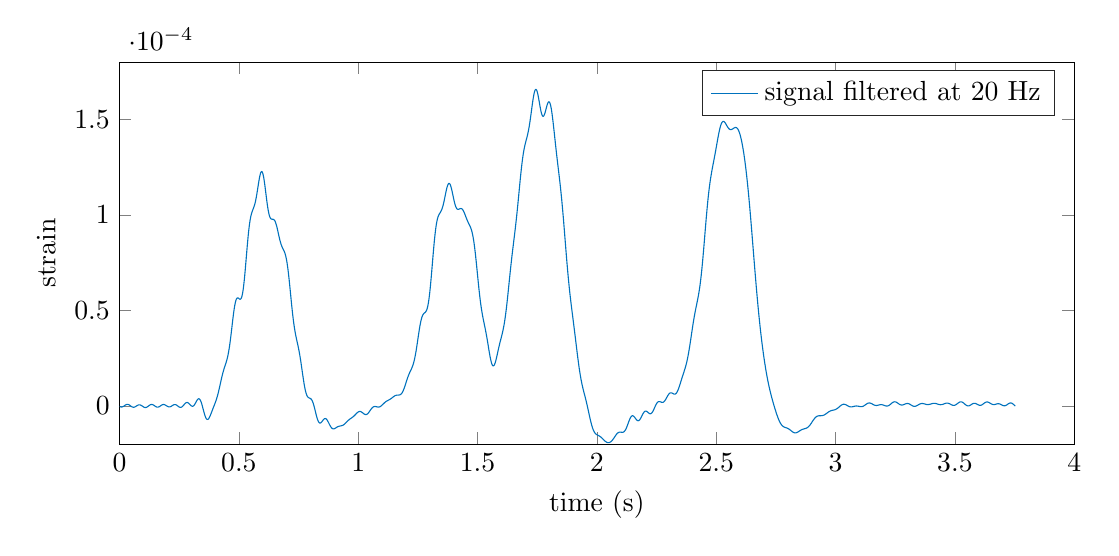
\begin{tikzpicture}

\begin{axis}[%
  width=\textwidth,
  height=0.4\textwidth,
  at={(0\figurewidth,0\figureheight)},
scale only axis,
xmin=0,
xmax=4,
xlabel={time (s)},
ymin=-2e-05,
ymax=0.00018,
ylabel={strain},
axis background/.style={fill=white},
legend style={legend cell align=left,align=left,draw=white!15!black}
]
\addplot [color=mycolor1,solid]
  table[row sep=crcr]{%
0	-1.64914494782242e-07\\
0.0009765625	-2.50432487527659e-07\\
0.001953125	-3.27443972509496e-07\\
0.0029296875	-3.9510375069788e-07\\
0.00390625	-4.5269234472603e-07\\
0.0048828125	-4.99625886845566e-07\\
0.005859375	-5.35464137854761e-07\\
0.0068359375	-5.59916519508564e-07\\
0.0078125	-5.7284607082382e-07\\
0.0087890625	-5.74271267963209e-07\\
0.009765625	-5.64365677601347e-07\\
0.0107421875	-5.43455444413984e-07\\
0.01171875	-5.12014644147333e-07\\
0.0126953125	-4.70658564175154e-07\\
0.013671875	-4.20135003098479e-07\\
0.0146484375	-3.61313709357627e-07\\
0.015625	-2.95174105595573e-07\\
0.0166015625	-2.22791470248774e-07\\
0.017578125	-1.45321770179538e-07\\
0.0185546875	-6.39853577811112e-08\\
0.01953125	1.99502374118287e-08\\
0.0205078125	1.0518817923402e-07\\
0.021484375	1.90420604267246e-07\\
0.0224609375	2.74347050564892e-07\\
0.0234375	3.55692773647188e-07\\
0.0244140625	4.33226688895029e-07\\
0.025390625	5.05778684423687e-07\\
0.0263671875	5.72256057159373e-07\\
0.02734375	6.3165883705505e-07\\
0.0283203125	6.83093780000739e-07\\
0.029296875	7.25786828788346e-07\\
0.0302734375	7.59093863219686e-07\\
0.03125	7.82509584790405e-07\\
0.0322265625	7.95674407997321e-07\\
0.033203125	7.98379258821543e-07\\
0.0341796875	7.90568210928591e-07\\
0.03515625	7.72338921167517e-07\\
0.0361328125	7.43940857598737e-07\\
0.037109375	7.05771345077046e-07\\
0.0380859375	6.58369484904312e-07\\
0.0390625	6.02408035786626e-07\\
0.0400390625	5.38683372840155e-07\\
0.041015625	4.68103669255719e-07\\
0.0419921875	3.91675471049882e-07\\
0.04296875	3.10488858720267e-07\\
0.0439453125	2.25701410241712e-07\\
0.044921875	1.38521197383983e-07\\
0.0458984375	5.01890615394151e-08\\
0.046875	-3.80395740906235e-08\\
0.0478515625	-1.24913092151551e-07\\
0.048828125	-2.0920200170126e-07\\
0.0498046875	-2.89716925489966e-07\\
0.05078125	-3.65325992361667e-07\\
0.0517578125	-4.34971381593947e-07\\
0.052734375	-4.97684778093421e-07\\
0.0537109375	-5.52601512986671e-07\\
0.0546875	-5.98973183069408e-07\\
0.0556640625	-6.36178564531748e-07\\
0.056640625	-6.63732661048796e-07\\
0.0576171875	-6.81293753361178e-07\\
0.05859375	-6.88668346477174e-07\\
0.0595703125	-6.85813941191068e-07\\
0.060546875	-6.7283958828428e-07\\
0.0615234375	-6.50004216102113e-07\\
0.0625	-6.17712754703574e-07\\
0.0634765625	-5.76510111995653e-07\\
0.064453125	-5.27073088713387e-07\\
0.0654296875	-4.70200349333146e-07\\
0.06640625	-4.06800594566038e-07\\
0.0673828125	-3.3787910754938e-07\\
0.068359375	-2.64522869849895e-07\\
0.0693359375	-1.87884464552289e-07\\
0.0703125	-1.09165001722677e-07\\
0.0712890625	-2.95963161349373e-08\\
0.072265625	4.95773018889892e-08\\
0.0732421875	1.27117574511833e-07\\
0.07421875	2.01810632026923e-07\\
0.0751953125	2.72485065577583e-07\\
0.076171875	3.38029371095752e-07\\
0.0771484375	3.97408527193842e-07\\
0.078125	4.49679462116374e-07\\
0.0791015625	4.94005180840218e-07\\
0.080078125	5.29667342775843e-07\\
0.0810546875	5.56077102991132e-07\\
0.08203125	5.72784055126509e-07\\
0.0830078125	5.79483141834685e-07\\
0.083984375	5.76019428254449e-07\\
0.0849609375	5.62390665287e-07\\
0.0859375	5.38747601827991e-07\\
0.0869140625	5.05392038145524e-07\\
0.087890625	4.62772645799838e-07\\
0.0888671875	4.11478612389332e-07\\
0.08984375	3.52231201490353e-07\\
0.0908203125	2.85873348970619e-07\\
0.091796875	2.13357445934573e-07\\
0.0927734375	1.35731485479067e-07\\
0.09375	5.41237747959819e-08\\
0.0947265625	-3.02735644054109e-08\\
0.095703125	-1.16222065992738e-07\\
0.0966796875	-2.02455104183775e-07\\
0.09765625	-2.87696526227154e-07\\
0.0986328125	-3.70679459193879e-07\\
0.099609375	-4.50165014075521e-07\\
0.1005859375	-5.24960611449581e-07\\
0.1015625	-5.93937658098327e-07\\
0.1025390625	-6.56048313089179e-07\\
0.103515625	-7.10341094814193e-07\\
0.1044921875	-7.55975097160125e-07\\
0.10546875	-7.92232603099135e-07\\
0.1064453125	-8.18529907266032e-07\\
0.107421875	-8.34426185180055e-07\\
0.1083984375	-8.39630275303355e-07\\
0.109375	-8.34005270683098e-07\\
0.1103515625	-8.1757084905702e-07\\
0.111328125	-7.90503303540797e-07\\
0.1123046875	-7.53133269869763e-07\\
0.11328125	-7.05941180143385e-07\\
0.1142578125	-6.49550506611002e-07\\
0.115234375	-5.84718891751962e-07\\
0.1162109375	-5.12327292251128e-07\\
0.1171875	-4.33367293991862e-07\\
0.1181640625	-3.48926782437959e-07\\
0.119140625	-2.6017417735232e-07\\
0.1201171875	-1.68341462329256e-07\\
0.12109375	-7.47062577794243e-08\\
0.1220703125	1.94267994759345e-08\\
0.123046875	1.12745096192748e-07\\
0.1240234375	2.03947221844005e-07\\
0.125	2.91762003997646e-07\\
0.1259765625	3.74967118715529e-07\\
0.126953125	4.52407000619224e-07\\
0.1279296875	5.23009787216839e-07\\
0.12890625	5.85803045981654e-07\\
0.1298828125	6.39928050318563e-07\\
0.130859375	6.84652391695341e-07\\
0.1318359375	7.19380739546387e-07\\
0.1328125	7.43663587721246e-07\\
0.1337890625	7.57203855854274e-07\\
0.134765625	7.59861245638474e-07\\
0.1357421875	7.51654285133861e-07\\
0.13671875	7.32760028436708e-07\\
0.1376953125	7.03511412779549e-07\\
0.138671875	6.64392309903511e-07\\
0.1396484375	6.16030342832313e-07\\
0.140625	5.59187572467514e-07\\
0.1416015625	4.94749190223642e-07\\
0.142578125	4.23710382750262e-07\\
0.1435546875	3.47161562202688e-07\\
0.14453125	2.66272180106538e-07\\
0.1455078125	1.82273364245708e-07\\
0.146484375	9.64396358614588e-08\\
0.1474609375	1.00699785084054e-08\\
0.1484375	-7.55314600441812e-08\\
0.1494140625	-1.59074745610844e-07\\
0.150390625	-2.39303326238289e-07\\
0.1513671875	-3.15012705564501e-07\\
0.15234375	-3.85068341733809e-07\\
0.1533203125	-4.48422503878025e-07\\
0.154296875	-5.04129833362214e-07\\
0.1552734375	-5.51361375986531e-07\\
0.15625	-5.89416873861349e-07\\
0.1572265625	-6.17735131400103e-07\\
0.158203125	-6.35902298429614e-07\\
0.1591796875	-6.4365794437824e-07\\
0.16015625	-6.40898830414305e-07\\
0.1611328125	-6.27680320780477e-07\\
0.162109375	-6.04215409896089e-07\\
0.1630859375	-5.70871377552119e-07\\
0.1640625	-5.28164120167906e-07\\
0.1650390625	-4.76750241081454e-07\\
0.166015625	-4.17417016681927e-07\\
0.1669921875	-3.51070387350014e-07\\
0.16796875	-2.787211521679e-07\\
0.1689453125	-2.01469573735701e-07\\
0.169921875	-1.20488623770328e-07\\
0.1708984375	-3.70061210920644e-08\\
0.171875	4.77139692012634e-08\\
0.1728515625	1.32390793379689e-07\\
0.173828125	2.15746132573588e-07\\
0.1748046875	2.96523896519069e-07\\
0.17578125	3.73509291784321e-07\\
0.1767578125	4.45547372983834e-07\\
0.177734375	5.11560694174132e-07\\
0.1787109375	5.70565790603231e-07\\
0.1796875	6.21688238072138e-07\\
0.1806640625	6.64176058119347e-07\\
0.181640625	6.97411261755314e-07\\
0.1826171875	7.20919352193587e-07\\
0.18359375	7.34376637546522e-07\\
0.1845703125	7.37615237322513e-07\\
0.185546875	7.30625701293311e-07\\
0.1865234375	7.13557195377225e-07\\
0.1875	6.86715246068231e-07\\
0.1884765625	6.50557072078082e-07\\
0.189453125	6.05684568691251e-07\\
0.1904296875	5.52835046302457e-07\\
0.19140625	4.92869859168548e-07\\
0.1923828125	4.26761093034445e-07\\
0.193359375	3.55576510484536e-07\\
0.1943359375	2.80462980163138e-07\\
0.1953125	2.02628639974761e-07\\
0.1962890625	1.23324064642259e-07\\
0.197265625	4.38227242455701e-08\\
0.1982421875	-3.45989676750169e-08\\
0.19921875	-1.10681710391802e-07\\
0.2001953125	-1.83203167719464e-07\\
0.201171875	-2.50997308104837e-07\\
0.2021484375	-3.12972932476768e-07\\
0.203125	-3.6813110035197e-07\\
0.2041015625	-4.15581180241601e-07\\
0.205078125	-4.5455527019192e-07\\
0.2060546875	-4.84420758041278e-07\\
0.20703125	-5.04690818346967e-07\\
0.2080078125	-5.15032673533071e-07\\
0.208984375	-5.15273480188213e-07\\
0.2099609375	-5.05403737109743e-07\\
0.2109375	-4.85578149123272e-07\\
0.2119140625	-4.56113919343701e-07\\
0.212890625	-4.17486481812631e-07\\
0.2138671875	-3.70322725753585e-07\\
0.21484375	-3.15391801440551e-07\\
0.2158203125	-2.53593635284567e-07\\
0.216796875	-1.85945317636198e-07\\
0.2177734375	-1.13565560423873e-07\\
0.21875	-3.76574525794951e-08\\
0.2197265625	4.05102312403177e-08\\
0.220703125	1.19622889279328e-07\\
0.2216796875	1.98340819541038e-07\\
0.22265625	2.75320500428329e-07\\
0.2236328125	3.49236100046107e-07\\
0.224609375	4.18800883249031e-07\\
0.2255859375	4.82788184702933e-07\\
0.2265625	5.40051620442454e-07\\
0.2275390625	5.89544219621334e-07\\
0.228515625	6.30336172258767e-07\\
0.2294921875	6.61630907605413e-07\\
0.23046875	6.82779241035955e-07\\
0.2314453125	6.93291354800451e-07\\
0.232421875	6.92846409150018e-07\\
0.2333984375	6.81299614852426e-07\\
0.234375	6.58686635431662e-07\\
0.2353515625	6.25225227065187e-07\\
0.236328125	5.81314065370653e-07\\
0.2373046875	5.27528750706341e-07\\
0.23828125	4.64615026463746e-07\\
0.2392578125	3.93479287511355e-07\\
0.240234375	3.15176497808278e-07\\
0.2412109375	2.30895676618075e-07\\
0.2421875	1.41943151091967e-07\\
0.2431640625	4.97238086737411e-08\\
0.244140625	-4.42793847543913e-08\\
0.2451171875	-1.38527306322803e-07\\
0.24609375	-2.31447718003375e-07\\
0.2470703125	-3.21459089623401e-07\\
0.248046875	-4.06994848820323e-07\\
0.2490234375	-4.86527693824396e-07\\
0.25	-5.58593600463293e-07\\
0.2509765625	-6.21815155773523e-07\\
0.251953125	-6.74923857110324e-07\\
0.2529296875	-7.16781027617758e-07\\
0.25390625	-7.46397016223642e-07\\
0.2548828125	-7.6294837274251e-07\\
0.255859375	-7.65792715920452e-07\\
0.2568359375	-7.54481043966106e-07\\
0.2578125	-7.28767272858494e-07\\
0.2587890625	-6.88614826999686e-07\\
0.259765625	-6.34200149045292e-07\\
0.2607421875	-5.65913040390039e-07\\
0.26171875	-4.84353790176486e-07\\
0.2626953125	-3.9032709815312e-07\\
0.263671875	-2.84832844551238e-07\\
0.2646484375	-1.69053807663221e-07\\
0.265625	-4.43404762964871e-08\\
0.2666015625	8.78068509580502e-08\\
0.267578125	2.25758445333701e-07\\
0.2685546875	3.67777732735555e-07\\
0.26953125	5.12045774511042e-07\\
0.2705078125	6.56687303351038e-07\\
0.271484375	7.99797946756639e-07\\
0.2724609375	9.39472248872876e-07\\
0.2734375	1.07383208535843e-06\\
0.2744140625	1.20105505561455e-06\\
0.275390625	1.31940243234017e-06\\
0.2763671875	1.42724625013209e-06\\
0.27734375	1.52309512273515e-06\\
0.2783203125	1.60561839251067e-06\\
0.279296875	1.67366823558019e-06\\
0.2802734375	1.72629937168027e-06\\
0.28125	1.76278605871025e-06\\
0.2822265625	1.78263608786784e-06\\
0.283203125	1.7856015356672e-06\\
0.2841796875	1.7716860734777e-06\\
0.28515625	1.74114868289666e-06\\
0.2861328125	1.6945036756199e-06\\
0.287109375	1.63251696878922e-06\\
0.2880859375	1.55619862034317e-06\\
0.2890625	1.46679168290783e-06\\
0.2900390625	1.36575748846814e-06\\
0.291015625	1.25475752867726e-06\\
0.2919921875	1.13563214642573e-06\\
0.29296875	1.01037630245815e-06\\
0.2939453125	8.8111272567801e-07\\
0.294921875	7.500627966483e-07\\
0.2958984375	6.19515550058997e-07\\
0.296875	4.91795213031571e-07\\
0.2978515625	3.6922772158093e-07\\
0.298828125	2.54106676941329e-07\\
0.2998046875	1.48659216464715e-07\\
0.30078125	5.50122801729874e-08\\
0.3017578125	-2.48402463464179e-08\\
0.302734375	-8.90690392241729e-08\\
0.3037109375	-1.36039034271872e-07\\
0.3046875	-1.64336876724944e-07\\
0.3056640625	-1.72795710843917e-07\\
0.306640625	-1.60516930477989e-07\\
0.3076171875	-1.26888550337315e-07\\
0.30859375	-7.15999014820409e-08\\
0.3095703125	5.34759717385617e-09\\
0.310546875	1.03633787371927e-07\\
0.3115234375	2.22617380717796e-07\\
0.3125	3.6133791151961e-07\\
0.3134765625	5.18522056824296e-07\\
0.314453125	6.92594287068799e-07\\
0.3154296875	8.8169175067557e-07\\
0.31640625	1.08368323673693e-06\\
0.3173828125	1.29619200249846e-06\\
0.318359375	1.51662219747836e-06\\
0.3193359375	1.74218856454587e-06\\
0.3203125	1.96994905086086e-06\\
0.3212890625	2.1968399189514e-06\\
0.322265625	2.41971291099058e-06\\
0.3232421875	2.63537398809323e-06\\
0.32421875	2.84062314164919e-06\\
0.3251953125	3.03229475573157e-06\\
0.326171875	3.20729798874951e-06\\
0.3271484375	3.36265663894807e-06\\
0.328125	3.4955479621746e-06\\
0.3291015625	3.60333992151715e-06\\
0.330078125	3.68362636685106e-06\\
0.3310546875	3.73425966778165e-06\\
0.33203125	3.75338035561451e-06\\
0.3330078125	3.73944336840289e-06\\
0.333984375	3.69124053729644e-06\\
0.3349609375	3.6079190017558e-06\\
0.3359375	3.48899529502615e-06\\
0.3369140625	3.33436489884808e-06\\
0.337890625	3.14430712692526e-06\\
0.3388671875	2.91948525933484e-06\\
0.33984375	2.66094191397642e-06\\
0.3408203125	2.37008970542911e-06\\
0.341796875	2.04869730530818e-06\\
0.3427734375	1.69887108050399e-06\\
0.34375	1.32303254565129e-06\\
0.3447265625	9.23891922984608e-07\\
0.345703125	5.04418155565683e-07\\
0.3466796875	6.78057679826272e-08\\
0.34765625	-3.82560988679007e-07\\
0.3486328125	-8.43146234109176e-07\\
0.349609375	-1.31030229467155e-06\\
0.3505859375	-1.78031075115584e-06\\
0.3515625	-2.2494241557799e-06\\
0.3525390625	-2.71390786755924e-06\\
0.353515625	-3.17008145456216e-06\\
0.3544921875	-3.61435911866714e-06\\
0.35546875	-4.04328861314289e-06\\
0.3564453125	-4.45358814547736e-06\\
0.357421875	-4.84218078708459e-06\\
0.3583984375	-5.20622594740534e-06\\
0.359375	-5.54314751198624e-06\\
0.3603515625	-5.85065829177096e-06\\
0.361328125	-6.12678048339747e-06\\
0.3623046875	-6.36986189700901e-06\\
0.36328125	-6.5785877681533e-06\\
0.3642578125	-6.75198803289778e-06\\
0.365234375	-6.88944000943829e-06\\
0.3662109375	-6.99066649429887e-06\\
0.3671875	-7.05572934578416e-06\\
0.3681640625	-7.08501869072021e-06\\
0.369140625	-7.07923795179377e-06\\
0.3701171875	-7.03938495108704e-06\\
0.37109375	-6.96672939986546e-06\\
0.3720703125	-6.86278713451764e-06\\
0.373046875	-6.72929150305238e-06\\
0.3740234375	-6.56816234507501e-06\\
0.375	-6.38147304014324e-06\\
0.3759765625	-6.17141612436532e-06\\
0.376953125	-5.94026799269937e-06\\
0.3779296875	-5.69035321437257e-06\\
0.37890625	-5.42400899102967e-06\\
0.3798828125	-5.14355028159876e-06\\
0.380859375	-4.85123610452078e-06\\
0.3818359375	-4.54923750711461e-06\\
0.3828125	-4.23960766375763e-06\\
0.3837890625	-3.92425452965571e-06\\
0.384765625	-3.60491643578346e-06\\
0.3857421875	-3.28314096368888e-06\\
0.38671875	-2.96026738698512e-06\\
0.3876953125	-2.63741291025117e-06\\
0.388671875	-2.31546287657547e-06\\
0.3896484375	-1.99506505297977e-06\\
0.390625	-1.67662803938561e-06\\
0.3916015625	-1.3603237825761e-06\\
0.392578125	-1.04609411273075e-06\\
0.3935546875	-7.33661157523197e-07\\
0.39453125	-4.2254142842234e-07\\
0.3955078125	-1.12063316633057e-07\\
0.396484375	1.98612317071002e-07\\
0.3974609375	5.10468822726267e-07\\
0.3984375	8.24608118652115e-07\\
0.3994140625	1.14222316944518e-06\\
0.400390625	1.46456905765398e-06\\
0.4013671875	1.79293314474506e-06\\
0.40234375	2.12860483177057e-06\\
0.4033203125	2.47284543704757e-06\\
0.404296875	2.82685870701538e-06\\
0.4052734375	3.19176246724298e-06\\
0.40625	3.56856190340633e-06\\
0.4072265625	3.95812493717978e-06\\
0.408203125	4.36116012971777e-06\\
0.4091796875	4.77819750620354e-06\\
0.41015625	5.20957264936378e-06\\
0.4111328125	5.65541435855565e-06\\
0.412109375	6.11563611476927e-06\\
0.4130859375	6.58993153148581e-06\\
0.4140625	7.07777390767912e-06\\
0.4150390625	7.57841993330104e-06\\
0.416015625	8.09091753033225e-06\\
0.4169921875	8.61411774493364e-06\\
0.41796875	9.14669053942034e-06\\
0.4189453125	9.68714426773128e-06\\
0.419921875	1.02338485557831e-05\\
0.4208984375	1.0785060249554e-05\\
0.421875	1.13389520398637e-05\\
0.4228515625	1.18936433244584e-05\\
0.423828125	1.24472328259698e-05\\
0.4248046875	1.29978324492801e-05\\
0.42578125	1.35436018344056e-05\\
0.4267578125	1.40827830416889e-05\\
0.427734375	1.46137347952474e-05\\
0.4287109375	1.51349657085168e-05\\
0.4296875	1.56451659224707e-05\\
0.4306640625	1.61432366026974e-05\\
0.431640625	1.6628316765826e-05\\
0.4326171875	1.70998069385583e-05\\
0.43359375	1.75573891933786e-05\\
0.4345703125	1.80010431533708e-05\\
0.435546875	1.84310576138298e-05\\
0.4365234375	1.88480374897774e-05\\
0.4375	1.92529058652349e-05\\
0.4384765625	1.96469009912462e-05\\
0.439453125	2.00315681541711e-05\\
0.4404296875	2.04087464126358e-05\\
0.44140625	2.07805502796098e-05\\
0.4423828125	2.11493465042506e-05\\
0.443359375	2.1517726185265e-05\\
0.4443359375	2.18884725224281e-05\\
0.4453125	2.22645245844544e-05\\
0.4462890625	2.26489375385316e-05\\
0.447265625	2.30448398484742e-05\\
0.4482421875	2.34553880036516e-05\\
0.44921875	2.38837193887026e-05\\
0.4501953125	2.43329039437858e-05\\
0.451171875	2.48058952960215e-05\\
0.4521484375	2.53054820643174e-05\\
0.453125	2.5834240051478e-05\\
0.4541015625	2.63944860390819e-05\\
0.455078125	2.69882338919172e-05\\
0.4560546875	2.7617153659768e-05\\
0.45703125	2.82825343351792e-05\\
0.4580078125	2.89852508867806e-05\\
0.458984375	2.97257361392289e-05\\
0.4599609375	3.05039580134085e-05\\
0.4609375	3.13194025748996e-05\\
0.4619140625	3.21710632657028e-05\\
0.462890625	3.30574366147279e-05\\
0.4638671875	3.39765246376591e-05\\
0.46484375	3.49258440476005e-05\\
0.4658203125	3.59024423056071e-05\\
0.466796875	3.69029204460467e-05\\
0.4677734375	3.79234625170246e-05\\
0.46875	3.89598713821476e-05\\
0.4697265625	4.00076105380214e-05\\
0.470703125	4.10618515133787e-05\\
0.4716796875	4.21175263318869e-05\\
0.47265625	4.31693844427125e-05\\
0.4736328125	4.42120534519723e-05\\
0.474609375	4.52401029253464e-05\\
0.4755859375	4.62481104783347e-05\\
0.4765625	4.72307293267494e-05\\
0.4775390625	4.81827564367866e-05\\
0.478515625	4.90992003919797e-05\\
0.4794921875	4.99753480839506e-05\\
0.48046875	5.08068293354179e-05\\
0.4814453125	5.15896785775077e-05\\
0.482421875	5.23203927290012e-05\\
0.4833984375	5.29959844625292e-05\\
0.484375	5.36140300915099e-05\\
0.4853515625	5.41727113712891e-05\\
0.486328125	5.46708505777963e-05\\
0.4873046875	5.51079383062291e-05\\
0.48828125	5.54841535198672e-05\\
0.4892578125	5.58003754739914e-05\\
0.490234375	5.60581872408423e-05\\
0.4912109375	5.62598706673075e-05\\
0.4921875	5.64083927061933e-05\\
0.4931640625	5.65073831730944e-05\\
0.494140625	5.65611040925461e-05\\
0.4951171875	5.6574410907844e-05\\
0.49609375	5.65527059371499e-05\\
0.4970703125	5.650188456281e-05\\
0.498046875	5.64282747397549e-05\\
0.4990234375	5.63385705010735e-05\\
0.5	5.62397602230608e-05\\
0.5009765625	5.61390504870481e-05\\
0.501953125	5.60437864400571e-05\\
0.5029296875	5.59613696098303e-05\\
0.50390625	5.58991741712853e-05\\
0.5048828125	5.58644626902662e-05\\
0.505859375	5.58643023861462e-05\\
0.5068359375	5.59054829570666e-05\\
0.5078125	5.59944370002405e-05\\
0.5087890625	5.61371640348696e-05\\
0.509765625	5.63391590970387e-05\\
0.5107421875	5.66053468248884e-05\\
0.51171875	5.6940021889e-05\\
0.5126953125	5.73467965480213e-05\\
0.513671875	5.78285560240219e-05\\
0.5146484375	5.83874222969602e-05\\
0.515625	5.90247268141622e-05\\
0.5166015625	5.97409925001667e-05\\
0.517578125	6.0535925336099e-05\\
0.5185546875	6.1408415657392e-05\\
0.51953125	6.23565491957376e-05\\
0.5205078125	6.33776277672301e-05\\
0.521484375	6.44681993853762e-05\\
0.5224609375	6.56240974566219e-05\\
0.5234375	6.68404885988784e-05\\
0.5244140625	6.81119285117886e-05\\
0.525390625	6.94324252226387e-05\\
0.5263671875	7.07955089353097e-05\\
0.52734375	7.21943076227726e-05\\
0.5283203125	7.36216274275489e-05\\
0.529296875	7.50700368703183e-05\\
0.5302734375	7.65319538153623e-05\\
0.53125	7.79997341034879e-05\\
0.5322265625	7.94657607390567e-05\\
0.533203125	8.09225325080862e-05\\
0.5341796875	8.23627509092933e-05\\
0.53515625	8.37794042993803e-05\\
0.5361328125	8.51658481876204e-05\\
0.537109375	8.65158806624816e-05\\
0.5380859375	8.78238119940439e-05\\
0.5390625	8.90845275295636e-05\\
0.5400390625	9.02935430847675e-05\\
0.541015625	9.14470521292482e-05\\
0.5419921875	9.25419641694407e-05\\
0.54296875	9.35759338457198e-05\\
0.5439453125	9.45473803797204e-05\\
0.544921875	9.54554971324751e-05\\
0.5458984375	9.63002511617647e-05\\
0.546875	9.70823727965163e-05\\
0.5478515625	9.78033353754594e-05\\
0.548828125	9.84653254248614e-05\\
0.5498046875	9.90712036743326e-05\\
0.55078125	9.96244574287765e-05\\
0.5517578125	0.000100129144926991\\
0.552734375	0.000100589832421709\\
0.5537109375	0.000101011524810646\\
0.5546875	0.000101399590732066\\
0.5556640625	0.000101759683110505\\
0.556640625	0.000102097656197471\\
0.5576171875	0.000102419480197537\\
0.55859375	0.000102731154601542\\
0.5595703125	0.000103038621365262\\
0.560546875	0.000103347679073603\\
0.5615234375	0.000103663899217191\\
0.5625	0.000103992545680205\\
0.5634765625	0.000104338498495914\\
0.564453125	0.000104706182870133\\
0.5654296875	0.000105099504403431\\
0.56640625	0.000105521791361366\\
0.5673828125	0.000105975744749318\\
0.568359375	0.000106463396845907\\
0.5693359375	0.000106986078737817\\
0.5703125	0.000107544397280645\\
0.5712890625	0.000108138221786627\\
0.572265625	0.000108766680612484\\
0.5732421875	0.000109428167690792\\
0.57421875	0.000110120358917981\\
0.5751953125	0.000110840238182994\\
0.576171875	0.000111584132694509\\
0.5771484375	0.000112347757143108\\
0.578125	0.000113126266119452\\
0.5791015625	0.000113914314101922\\
0.580078125	0.000114706122228748\\
0.5810546875	0.000115495550981589\\
0.58203125	0.000116276177831096\\
0.5830078125	0.000117041378831115\\
0.583984375	0.000117784413097696\\
0.5849609375	0.000118498509072689\\
0.5859375	0.000119176951449756\\
0.5869140625	0.000119813167633563\\
0.587890625	0.000120400812610582\\
0.5888671875	0.000120933851132441\\
0.58984375	0.000121406636149571\\
0.5908203125	0.000121813982483675\\
0.591796875	0.000122151234791454\\
0.5927734375	0.000122414328948269\\
0.59375	0.000122599846067986\\
0.5947265625	0.000122705058472824\\
0.595703125	0.000122727967033482\\
0.5966796875	0.000122667329413571\\
0.59765625	0.000122522678871954\\
0.5986328125	0.000122294333400456\\
0.599609375	0.00012198339510076\\
0.6005859375	0.000121591739831638\\
0.6015625	0.000121121997284129\\
0.6025390625	0.000120577521766344\\
0.603515625	0.000119962354099435\\
0.6044921875	0.000119281175140566\\
0.60546875	0.000118539251555693\\
0.6064453125	0.000117742374563465\\
0.607421875	0.000116896792460134\\
0.6083984375	0.00011600913781292\\
0.609375	0.000115086350274891\\
0.6103515625	0.000114135596027122\\
0.611328125	0.000113164184893193\\
0.6123046875	0.00011217948619634\\
0.61328125	0.000111188844440653\\
0.6142578125	0.000110199495894414\\
0.615234375	0.000109218487136139\\
0.6162109375	0.000108252596592427\\
0.6171875	0.000107308260051766\\
0.6181640625	0.000106391501080707\\
0.619140625	0.000105507867199054\\
0.6201171875	0.000104662372589982\\
0.62109375	0.000103859448030381\\
0.6220703125	0.000103102898627452\\
0.623046875	0.00010239586984111\\
0.6240234375	0.000101740822159449\\
0.625	0.000101139514677963\\
0.6259765625	0.000100592997713995\\
0.626953125	0.000100101614467584\\
0.6279296875	9.9665011620144e-05\\
0.62890625	9.92821586447956e-05\\
0.6298828125	9.89513754883646e-05\\
0.630859375	9.8670368176401e-05\\
0.6318359375	9.84362717906716e-05\\
0.6328125	9.82457001746457e-05\\
0.6337890625	9.80948016378273e-05\\
0.634765625	9.79793198554442e-05\\
0.6357421875	9.7894659096952e-05\\
0.63671875	9.78359528658347e-05\\
0.6376953125	9.77981349949089e-05\\
0.638671875	9.77760122162146e-05\\
0.6396484375	9.77643372128729e-05\\
0.640625	9.7757881162095e-05\\
0.6416015625	9.77515047937367e-05\\
0.642578125	9.77402270171305e-05\\
0.6435546875	9.77192902099393e-05\\
0.64453125	9.76842213158246e-05\\
0.6455078125	9.76308879620299e-05\\
0.646484375	9.75555488826045e-05\\
0.6474609375	9.74548980168568e-05\\
0.6484375	9.73261017445411e-05\\
0.6494140625	9.71668288179453e-05\\
0.650390625	9.69752726550714e-05\\
0.6513671875	9.67501657660441e-05\\
0.65234375	9.64907861952354e-05\\
0.6533203125	9.61969559728416e-05\\
0.654296875	9.58690316802623e-05\\
0.6552734375	9.55078873420912e-05\\
0.65625	9.51148899623734e-05\\
0.6572265625	9.46918681225796e-05\\
0.658203125	9.42410741521652e-05\\
0.6591796875	9.37651404683651e-05\\
0.66015625	9.32670307588911e-05\\
0.6611328125	9.27499867484288e-05\\
0.662109375	9.22174713464144e-05\\
0.6630859375	9.16731090187753e-05\\
0.6640625	9.11206242595836e-05\\
0.6650390625	9.05637790595107e-05\\
0.666015625	9.00063102763441e-05\\
0.6669921875	8.94518678086031e-05\\
0.66796875	8.89039544565758e-05\\
0.6689453125	8.83658683262002e-05\\
0.669921875	8.78406485905873e-05\\
0.6708984375	8.73310253722465e-05\\
0.671875	8.68393744470081e-05\\
0.6728515625	8.63676773991395e-05\\
0.673828125	8.59174877772628e-05\\
0.6748046875	8.54899037135516e-05\\
0.67578125	8.50855473755406e-05\\
0.6767578125	8.47045515220607e-05\\
0.677734375	8.43465533336676e-05\\
0.6787109375	8.40106955849007e-05\\
0.6796875	8.36956351222108e-05\\
0.6806640625	8.33995585088714e-05\\
0.681640625	8.31202045980545e-05\\
0.6826171875	8.28548936988782e-05\\
0.68359375	8.2600562908946e-05\\
0.6845703125	8.23538071019259e-05\\
0.685546875	8.21109249812237e-05\\
0.6865234375	8.18679695418139e-05\\
0.6875	8.16208022227343e-05\\
0.6884765625	8.13651499834044e-05\\
0.689453125	8.10966644984289e-05\\
0.6904296875	8.08109826383888e-05\\
0.69140625	8.05037873886294e-05\\
0.6923828125	8.01708683543854e-05\\
0.693359375	7.98081810087519e-05\\
0.6943359375	7.94119038598382e-05\\
0.6953125	7.89784927446215e-05\\
0.6962890625	7.85047314990562e-05\\
0.697265625	7.79877783062813e-05\\
0.6982421875	7.74252070865197e-05\\
0.69921875	7.68150433626061e-05\\
0.7001953125	7.61557941129888e-05\\
0.701171875	7.5446471208432e-05\\
0.7021484375	7.46866081182991e-05\\
0.703125	7.38762696659629e-05\\
0.7041015625	7.30160547092647e-05\\
0.705078125	7.21070917196771e-05\\
0.7060546875	7.1151027331572e-05\\
0.70703125	7.01500080293965e-05\\
0.7080078125	6.91066552342998e-05\\
0.708984375	6.80240341415421e-05\\
0.7099609375	6.69056167446401e-05\\
0.7109375	6.57552395605086e-05\\
0.7119140625	6.45770566407916e-05\\
0.712890625	6.33754885172003e-05\\
0.7138671875	6.2155167782148e-05\\
0.71484375	6.09208820496028e-05\\
0.7158203125	5.96775150743073e-05\\
0.716796875	5.84299868299214e-05\\
0.7177734375	5.71831933579723e-05\\
0.71875	5.59419471996297e-05\\
0.7197265625	5.47109192113128e-05\\
0.720703125	5.34945825431796e-05\\
0.7216796875	5.22971595269873e-05\\
0.72265625	5.11225721771513e-05\\
0.7236328125	4.99743969566896e-05\\
0.724609375	4.88558243988801e-05\\
0.7255859375	4.7769624106754e-05\\
0.7265625	4.67181155769834e-05\\
0.7275390625	4.570314521335e-05\\
0.728515625	4.47260698089656e-05\\
0.7294921875	4.37877466869401e-05\\
0.73046875	4.28885305975175e-05\\
0.7314453125	4.2028277377077e-05\\
0.732421875	4.12063542821232e-05\\
0.7333984375	4.0421656820708e-05\\
0.734375	3.96726318158928e-05\\
0.7353515625	3.89573063520583e-05\\
0.736328125	3.82733221762318e-05\\
0.7373046875	3.76179750541838e-05\\
0.73828125	3.69882585158195e-05\\
0.7392578125	3.6380911367202e-05\\
0.740234375	3.57924682981582e-05\\
0.7412109375	3.52193128754423e-05\\
0.7421875	3.46577321823643e-05\\
0.7431640625	3.41039723469823e-05\\
0.744140625	3.3554294192612e-05\\
0.7451171875	3.30050282465949e-05\\
0.74609375	3.24526283559026e-05\\
0.7470703125	3.18937231810176e-05\\
0.748046875	3.13251648722555e-05\\
0.7490234375	3.07440742747834e-05\\
0.75	3.0147882059423e-05\\
0.7509765625	2.95343652351624e-05\\
0.751953125	2.8901678565293e-05\\
0.7529296875	2.82483804812988e-05\\
0.75390625	2.75734531660292e-05\\
0.7548828125	2.68763165592083e-05\\
0.755859375	2.61568361228177e-05\\
0.7568359375	2.54153242901876e-05\\
0.7578125	2.46525356095276e-05\\
0.7587890625	2.38696556789535e-05\\
0.759765625	2.3068284054623e-05\\
0.7607421875	2.22504113952445e-05\\
0.76171875	2.14183911838671e-05\\
0.7626953125	2.05749064404435e-05\\
0.763671875	1.9722931905232e-05\\
0.7646484375	1.88656922327778e-05\\
0.765625	1.80066167882077e-05\\
0.7666015625	1.71492916812295e-05\\
0.767578125	1.6297409707976e-05\\
0.7685546875	1.54547188962646e-05\\
0.76953125	1.462497036565e-05\\
0.7705078125	1.38118662196651e-05\\
0.771484375	1.30190081838548e-05\\
0.7724609375	1.22498476896997e-05\\
0.7734375	1.15076380815565e-05\\
0.7744140625	1.07953895916593e-05\\
0.775390625	1.01158276875303e-05\\
0.7763671875	9.47135534744108e-06\\
0.77734375	8.86401976354956e-06\\
0.7783203125	8.29548390982756e-06\\
0.779296875	7.76700334377267e-06\\
0.7802734375	7.27940853812588e-06\\
0.78125	6.83309296241666e-06\\
0.7822265625	6.42800705518372e-06\\
0.783203125	6.06365814727123e-06\\
0.7841796875	5.73911631577154e-06\\
0.78515625	5.4530260680861e-06\\
0.7861328125	5.20362367728675e-06\\
0.787109375	4.98875991453405e-06\\
0.7880859375	4.8059278527567e-06\\
0.7890625	4.65229534906472e-06\\
0.7900390625	4.52474175233335e-06\\
0.791015625	4.4198983278507e-06\\
0.7919921875	4.33419184356754e-06\\
0.79296875	4.26389072291919e-06\\
0.7939453125	4.20515313789557e-06\\
0.794921875	4.15407639338335e-06\\
0.7958984375	4.10674694004931e-06\\
0.796875	4.05929034829912e-06\\
0.7978515625	4.00792058013595e-06\\
0.798828125	3.94898790894331e-06\\
0.7998046875	3.87902485907899e-06\\
0.80078125	3.79478956734502e-06\\
0.8017578125	3.69330600641684e-06\\
0.802734375	3.57190055561264e-06\\
0.8037109375	3.42823445628716e-06\\
0.8046875	3.26033174690202e-06\\
0.8056640625	3.06660233562628e-06\\
0.806640625	2.84585993527534e-06\\
0.8076171875	2.59733465556291e-06\\
0.80859375	2.32068012005302e-06\\
0.8095703125	2.01597504885461e-06\\
0.810546875	1.68371932200206e-06\\
0.8115234375	1.32482461160662e-06\\
0.8125	9.40599742267551e-07\\
0.8134765625	5.32731007944117e-07\\
0.814453125	1.03257738610225e-07\\
0.8154296875	-3.45456529314365e-07\\
0.81640625	-8.10756869312763e-07\\
0.8173828125	-1.28973330894197e-06\\
0.818359375	-1.77926019989863e-06\\
0.8193359375	-2.27603807615968e-06\\
0.8203125	-2.77663743397625e-06\\
0.8212890625	-3.27754384691494e-06\\
0.822265625	-3.77520381657357e-06\\
0.8232421875	-4.26607075515369e-06\\
0.82421875	-4.74665049972919e-06\\
0.8251953125	-5.2135457696918e-06\\
0.826171875	-5.66349899824248e-06\\
0.8271484375	-6.09343299560445e-06\\
0.828125	-6.5004889354214e-06\\
0.8291015625	-6.88206119605474e-06\\
0.830078125	-7.23582863459609e-06\\
0.8310546875	-7.55978192269206e-06\\
0.83203125	-7.85224662898546e-06\\
0.8330078125	-8.11190179232459e-06\\
0.833984375	-8.33779379203173e-06\\
0.8349609375	-8.52934538559445e-06\\
0.8359375	-8.68635984925613e-06\\
0.8369140625	-8.80902022225266e-06\\
0.837890625	-8.89788371997855e-06\\
0.8388671875	-8.95387144431388e-06\\
0.83984375	-8.97825357985892e-06\\
0.8408203125	-8.97263032212674e-06\\
0.841796875	-8.93890883708643e-06\\
0.8427734375	-8.87927660016032e-06\\
0.84375	-8.7961715062502e-06\\
0.8447265625	-8.69224918007079e-06\\
0.845703125	-8.57034794756179e-06\\
0.8466796875	-8.43345195408069e-06\\
0.84765625	-8.28465293318331e-06\\
0.8486328125	-8.12711114092194e-06\\
0.849609375	-7.96401597465804e-06\\
0.8505859375	-7.79854679243731e-06\\
0.8515625	-7.63383443913063e-06\\
0.8525390625	-7.47292396903201e-06\\
0.853515625	-7.31873903172636e-06\\
0.8544921875	-7.17404835919726e-06\\
0.85546875	-7.04143475779946e-06\\
0.8564453125	-6.92326696942164e-06\\
0.857421875	-6.82167472250453e-06\\
0.8583984375	-6.73852724622121e-06\\
0.859375	-6.67541547075836e-06\\
0.8603515625	-6.63363808399678e-06\\
0.861328125	-6.61419156072088e-06\\
0.8623046875	-6.61776422556024e-06\\
0.86328125	-6.64473435593743e-06\\
0.8642578125	-6.69517227712694e-06\\
0.865234375	-6.76884634884471e-06\\
0.8662109375	-6.86523269229769e-06\\
0.8671875	-6.98352845898296e-06\\
0.8681640625	-7.12266839835778e-06\\
0.869140625	-7.28134444135772e-06\\
0.8701171875	-7.45802798111824e-06\\
0.87109375	-7.6509945015776e-06\\
0.8720703125	-7.85835017925734e-06\\
0.873046875	-8.0780600637009e-06\\
0.8740234375	-8.30797742799206e-06\\
0.875	-8.54587387257726e-06\\
0.8759765625	-8.7894697633058e-06\\
0.876953125	-9.03646458811532e-06\\
0.8779296875	-9.28456682599223e-06\\
0.87890625	-9.53152293650067e-06\\
0.8798828125	-9.77514509801939e-06\\
0.880859375	-1.00133373474788e-05\\
0.8818359375	-1.02441198034409e-05\\
0.8828125	-1.04656506873216e-05\\
0.8837890625	-1.06762458939031e-05\\
0.884765625	-1.08743959014427e-05\\
0.8857421875	-1.10587798530701e-05\\
0.88671875	-1.1228276684141e-05\\
0.8876953125	-1.13819732141605e-05\\
0.888671875	-1.15191691661543e-05\\
0.8896484375	-1.16393791203248e-05\\
0.890625	-1.17423314518552e-05\\
0.8916015625	-1.18279643442254e-05\\
0.892578125	-1.18964190088128e-05\\
0.8935546875	-1.19480302783332e-05\\
0.89453125	-1.19833147753628e-05\\
0.8955078125	-1.20029568873295e-05\\
0.896484375	-1.20077928056021e-05\\
0.8974609375	-1.19987929083312e-05\\
0.8984375	-1.19770427842543e-05\\
0.8994140625	-1.19437232075988e-05\\
0.900390625	-1.1900089382385e-05\\
0.9013671875	-1.1847449777822e-05\\
0.90234375	-1.17871448751192e-05\\
0.9033203125	-1.17205261400253e-05\\
0.904296875	-1.16489355249053e-05\\
0.9052734375	-1.15736857894178e-05\\
0.90625	-1.14960419101438e-05\\
0.9072265625	-1.14172038271833e-05\\
0.908203125	-1.13382907501789e-05\\
0.9091796875	-1.12603272178633e-05\\
0.91015625	-1.11842310745435e-05\\
0.9111328125	-1.11108034944054e-05\\
0.912109375	-1.10407211506787e-05\\
0.9130859375	-1.09745305920554e-05\\
0.9140625	-1.09126448538434e-05\\
0.9150390625	-1.0855342296683e-05\\
0.916015625	-1.08027676317715e-05\\
0.9169921875	-1.07549350589264e-05\\
0.91796875	-1.07117334129386e-05\\
0.9189453125	-1.06729331849615e-05\\
0.919921875	-1.06381952595437e-05\\
0.9208984375	-1.06070811847027e-05\\
0.921875	-1.05790647724482e-05\\
0.9228515625	-1.05535448106636e-05\\
0.923828125	-1.052985865442e-05\\
0.9248046875	-1.05072964557869e-05\\
0.92578125	-1.04851157860784e-05\\
0.9267578125	-1.04625564032645e-05\\
0.927734375	-1.04388549199385e-05\\
0.9287109375	-1.0413259133663e-05\\
0.9296875	-1.03850417915691e-05\\
0.9306640625	-1.03535135745443e-05\\
0.931640625	-1.03180351029621e-05\\
0.9326171875	-1.02780277853712e-05\\
0.93359375	-1.02329833535455e-05\\
0.9345703125	-1.01824719514117e-05\\
0.935546875	-1.01261486712186e-05\\
0.9365234375	-1.00637584574745e-05\\
0.9375	-9.99513932720137e-06\\
0.9384765625	-9.92022388350419e-06\\
0.939453125	-9.83903912786909e-06\\
0.9404296875	-9.75170460454963e-06\\
0.94140625	-9.65842893743756e-06\\
0.9423828125	-9.55950484553631e-06\\
0.943359375	-9.45530274716687e-06\\
0.9443359375	-9.34626308498422e-06\\
0.9453125	-9.23288752344057e-06\\
0.9462890625	-9.11572918721995e-06\\
0.947265625	-8.99538212314591e-06\\
0.9482421875	-8.87247017894089e-06\\
0.94921875	-8.74763549984736e-06\\
0.9501953125	-8.62152684842139e-06\\
0.951171875	-8.49478795373457e-06\\
0.9521484375	-8.36804609379223e-06\\
0.953125	-8.24190110925342e-06\\
0.9541015625	-8.11691503764509e-06\\
0.955078125	-7.99360254535902e-06\\
0.9560546875	-7.87242232002065e-06\\
0.95703125	-7.75376956857142e-06\\
0.9580078125	-7.63796974690729e-06\\
0.958984375	-7.52527362548151e-06\\
0.9599609375	-7.41585377226862e-06\\
0.9609375	-7.30980251026428e-06\\
0.9619140625	-7.20713138165973e-06\\
0.962890625	-7.10777212537403e-06\\
0.9638671875	-7.01157914916094e-06\\
0.96484375	-6.91833345243116e-06\\
0.9658203125	-6.8277479316382e-06\\
0.966796875	-6.73947397695106e-06\\
0.9677734375	-6.65310924733589e-06\\
0.96875	-6.56820649143093e-06\\
0.9697265625	-6.48428326402718e-06\\
0.970703125	-6.40083237283436e-06\\
0.9716796875	-6.3173328777467e-06\\
0.97265625	-6.23326145522063e-06\\
0.9736328125	-6.14810393377702e-06\\
0.974609375	-6.06136680314648e-06\\
0.9755859375	-5.97258849923698e-06\\
0.9765625	-5.88135026991932e-06\\
0.9775390625	-5.78728643255399e-06\\
0.978515625	-5.69009384312628e-06\\
0.9794921875	-5.58954040867569e-06\\
0.98046875	-5.48547248921839e-06\\
0.9814453125	-5.37782105234026e-06\\
0.982421875	-5.26660646282273e-06\\
0.9833984375	-5.15194181075952e-06\\
0.984375	-5.03403470430233e-06\\
0.9853515625	-4.91318747709368e-06\\
0.986328125	-4.78979578523526e-06\\
0.9873046875	-4.66434559392447e-06\\
0.98828125	-4.53740857928075e-06\\
0.9892578125	-4.40963599599107e-06\\
0.990234375	-4.28175108584545e-06\\
0.9912109375	-4.15454012563699e-06\\
0.9921875	-4.02884223490668e-06\\
0.9931640625	-3.90553808428702e-06\\
0.994140625	-3.7855376634264e-06\\
0.9951171875	-3.66976728338395e-06\\
0.99609375	-3.55915600171764e-06\\
0.9970703125	-3.45462166905177e-06\\
0.998046875	-3.35705680352581e-06\\
0.9990234375	-3.26731450408467e-06\\
1	-3.18619461498362e-06\\
1.0009765625	-3.11443035213093e-06\\
1.001953125	-3.05267559698423e-06\\
1.0029296875	-3.00149305572679e-06\\
1.00390625	-2.96134347047999e-06\\
1.0048828125	-2.93257605551573e-06\\
1.005859375	-2.91542031501334e-06\\
1.0068359375	-2.90997938009243e-06\\
1.0078125	-2.91622498191771e-06\\
1.0087890625	-2.93399415491589e-06\\
1.009765625	-2.96298773989355e-06\\
1.0107421875	-3.0027707314553e-06\\
1.01171875	-3.05277448795258e-06\\
1.0126953125	-3.11230079563344e-06\\
1.013671875	-3.1805277520892e-06\\
1.0146484375	-3.25651740789829e-06\\
1.015625	-3.33922507992529e-06\\
1.0166015625	-3.42751022541873e-06\\
1.017578125	-3.52014874321372e-06\\
1.0185546875	-3.61584654732346e-06\\
1.01953125	-3.71325423929719e-06\\
1.0205078125	-3.81098268921235e-06\\
1.021484375	-3.90761932129497e-06\\
1.0224609375	-4.00174488912895e-06\\
1.0234375	-4.09195051738534e-06\\
1.0244140625	-4.17685478209652e-06\\
1.025390625	-4.2551205997923e-06\\
1.0263671875	-4.32547169733547e-06\\
1.02734375	-4.38670843902605e-06\\
1.0283203125	-4.43772279542109e-06\\
1.029296875	-4.47751224923758e-06\\
1.0302734375	-4.50519244751239e-06\\
1.03125	-4.52000842569677e-06\\
1.0322265625	-4.52134424833112e-06\\
1.033203125	-4.50873093211183e-06\\
1.0341796875	-4.48185254023033e-06\\
1.03515625	-4.4405503615084e-06\\
1.0361328125	-4.38482511372924e-06\\
1.037109375	-4.3148371373042e-06\\
1.0380859375	-4.23090457264703e-06\\
1.0390625	-4.13349954196678e-06\\
1.0400390625	-4.02324238325291e-06\\
1.041015625	-3.90089401063363e-06\\
1.0419921875	-3.76734650066984e-06\\
1.04296875	-3.62361202814678e-06\\
1.0439453125	-3.47081029721029e-06\\
1.044921875	-3.31015463395148e-06\\
1.0458984375	-3.14293692449315e-06\\
1.046875	-2.9705115980247e-06\\
1.0478515625	-2.79427886685539e-06\\
1.048828125	-2.61566744524059e-06\\
1.0498046875	-2.43611697534606e-06\\
1.05078125	-2.25706039216779e-06\\
1.0517578125	-2.0799064594769e-06\\
1.052734375	-1.90602270591027e-06\\
1.0537109375	-1.73671898423e-06\\
1.0546875	-1.57323186761752e-06\\
1.0556640625	-1.41671008478869e-06\\
1.056640625	-1.26820118088784e-06\\
1.0576171875	-1.12863957375965e-06\\
1.05859375	-9.98836155554456e-07\\
1.0595703125	-8.7946956797718e-07\\
1.060546875	-7.71079256152733e-07\\
1.0615234375	-6.74060381381365e-07\\
1.0625	-5.88660647347679e-07\\
1.0634765625	-5.14979067988961e-07\\
1.064453125	-4.52966678595712e-07\\
1.0654296875	-4.02429165181945e-07\\
1.06640625	-3.63031361098537e-07\\
1.0673828125	-3.34303534633616e-07\\
1.068359375	-3.15649367299805e-07\\
1.0693359375	-3.06355499983847e-07\\
1.0703125	-3.05602503440508e-07\\
1.0712890625	-3.1247711103176e-07\\
1.072265625	-3.25985535400237e-07\\
1.0732421875	-3.45067677138176e-07\\
1.07421875	-3.6861202265426e-07\\
1.0751953125	-3.95471020488604e-07\\
1.076171875	-4.24476720383534e-07\\
1.0771484375	-4.54456457539776e-07\\
1.078125	-4.84248365686417e-07\\
1.0791015625	-5.12716506838736e-07\\
1.080078125	-5.38765412836454e-07\\
1.0810546875	-5.61353843827198e-07\\
1.08203125	-5.79507581633559e-07\\
1.0830078125	-5.92331091217837e-07\\
1.083984375	-5.99017901009789e-07\\
1.0849609375	-5.98859572425618e-07\\
1.0859375	-5.91253150194762e-07\\
1.0869140625	-5.75707007805631e-07\\
1.087890625	-5.5184502615861e-07\\
1.0888671875	-5.19409068017953e-07\\
1.08984375	-4.78259735736842e-07\\
1.0908203125	-4.28375424623548e-07\\
1.091796875	-3.69849708868667e-07\\
1.0927734375	-3.02887120805383e-07\\
1.09375	-2.27797407087293e-07\\
1.0947265625	-1.44988366816108e-07\\
1.095703125	-5.49573964252869e-08\\
1.0966796875	4.17181160497025e-08\\
1.09765625	1.44391389064767e-07\\
1.0986328125	2.52357666574607e-07\\
1.099609375	3.64866275913345e-07\\
1.1005859375	4.81133134661867e-07\\
1.1015625	6.0035351162745e-07\\
1.1025390625	7.21714844989195e-07\\
1.103515625	8.44409421527252e-07\\
1.1044921875	9.67646724635149e-07\\
1.10546875	1.09066526544365e-06\\
1.1064453125	1.21274372075803e-06\\
1.107421875	1.33321121348163e-06\\
1.1083984375	1.45145658558094e-06\\
1.109375	1.56693653022468e-06\\
1.1103515625	1.67918246825029e-06\\
1.111328125	1.78780607429293e-06\\
1.1123046875	1.89250337945837e-06\\
1.11328125	1.9930574000008e-06\\
1.1142578125	2.08933926474811e-06\\
1.115234375	2.18130783764922e-06\\
1.1162109375	2.26900785544647e-06\\
1.1171875	2.3525666237508e-06\\
1.1181640625	2.43218933736643e-06\\
1.119140625	2.5081531122406e-06\\
1.1201171875	2.58079983657636e-06\\
1.12109375	2.65052796714241e-06\\
1.1220703125	2.71778341336303e-06\\
1.123046875	2.78304966612364e-06\\
1.1240234375	2.84683734016389e-06\\
1.125	2.90967330826972e-06\\
1.1259765625	2.97208961207109e-06\\
1.126953125	3.03461233799908e-06\\
1.1279296875	3.09775064779248e-06\\
1.12890625	3.16198615084794e-06\\
1.1298828125	3.2277628007043e-06\\
1.130859375	3.29547749010472e-06\\
1.1318359375	3.36547150850005e-06\\
1.1328125	3.43802301269071e-06\\
1.1337890625	3.51334064574139e-06\\
1.134765625	3.59155842156629e-06\\
1.1357421875	3.67273197292943e-06\\
1.13671875	3.75683623932164e-06\\
1.1376953125	3.84376464857478e-06\\
1.138671875	3.93332982248694e-06\\
1.1396484375	4.0252658125106e-06\\
1.140625	4.11923184705617e-06\\
1.1416015625	4.21481754755743e-06\\
1.142578125	4.31154954649548e-06\\
1.1435546875	4.40889941744987e-06\\
1.14453125	4.50629280529261e-06\\
1.1455078125	4.60311962419988e-06\\
1.146484375	4.69874517254666e-06\\
1.1474609375	4.79252199726545e-06\\
1.1484375	4.88380232615454e-06\\
1.1494140625	4.97195087514982e-06\\
1.150390625	5.05635782891662e-06\\
1.1513671875	5.13645178743565e-06\\
1.15234375	5.2117124686586e-06\\
1.1533203125	5.28168295786874e-06\\
1.154296875	5.34598129811714e-06\\
1.1552734375	5.40431122300306e-06\\
1.15625	5.45647184304886e-06\\
1.1572265625	5.50236610988146e-06\\
1.158203125	5.54200789820909e-06\\
1.1591796875	5.5755275639775e-06\\
1.16015625	5.60317585786085e-06\\
1.1611328125	5.6253260961152e-06\\
1.162109375	5.6424745154842e-06\\
1.1630859375	5.65523876495928e-06\\
1.1640625	5.66435451439659e-06\\
1.1650390625	5.67067018789734e-06\\
1.166015625	5.67513985806807e-06\\
1.1669921875	5.67881436539022e-06\\
1.16796875	5.68283075452862e-06\\
1.1689453125	5.68840014609752e-06\\
1.169921875	5.69679418777467e-06\\
1.1708984375	5.70933025233034e-06\\
1.171875	5.72735557175123e-06\\
1.1728515625	5.7522305158506e-06\\
1.173828125	5.78531124025723e-06\\
1.1748046875	5.82793194219086e-06\\
1.17578125	5.88138697272421e-06\\
1.1767578125	5.946913061112e-06\\
1.177734375	6.02567191008341e-06\\
1.1787109375	6.11873342065048e-06\\
1.1796875	6.22705980093131e-06\\
1.1806640625	6.35149080572606e-06\\
1.181640625	6.49273034217125e-06\\
1.1826171875	6.6513346618399e-06\\
1.18359375	6.82770234130877e-06\\
1.1845703125	7.02206623168933e-06\\
1.185546875	7.23448753316523e-06\\
1.1865234375	7.46485212350128e-06\\
1.1875	7.71286924011838e-06\\
1.1884765625	7.97807258404826e-06\\
1.189453125	8.25982388129345e-06\\
1.1904296875	8.55731890325634e-06\\
1.19140625	8.86959591342124e-06\\
1.1923828125	9.19554647284477e-06\\
1.193359375	9.53392850270696e-06\\
1.1943359375	9.88338146868332e-06\\
1.1953125	1.02424435196863e-05\\
1.1962890625	1.06095703830631e-05\\
1.197265625	1.09831557900689e-05\\
1.1982421875	1.13615531797856e-05\\
1.19921875	1.17430984070197e-05\\
1.2001953125	1.2126133160448e-05\\
1.201171875	1.2509028781701e-05\\
1.2021484375	1.28902101644598e-05\\
1.203125	1.32681794052065e-05\\
1.2041015625	1.3641538874188e-05\\
1.205078125	1.40090133765338e-05\\
1.2060546875	1.43694710793718e-05\\
1.20703125	1.47219428911943e-05\\
1.2080078125	1.5065639994586e-05\\
1.208984375	1.53999692525978e-05\\
1.2099609375	1.57245462323503e-05\\
1.2109375	1.6039205616638e-05\\
1.2119140625	1.63440088050669e-05\\
1.212890625	1.66392485402543e-05\\
1.2138671875	1.69254504314368e-05\\
1.21484375	1.72033712870288e-05\\
1.2158203125	1.74739942087699e-05\\
1.216796875	1.77385204425734e-05\\
1.2177734375	1.79983580244955e-05\\
1.21875	1.82551073038372e-05\\
1.2197265625	1.85105434686782e-05\\
1.220703125	1.87665962415605e-05\\
1.2216796875	1.90253269540062e-05\\
1.22265625	1.92889032475087e-05\\
1.2236328125	1.95595716850329e-05\\
1.224609375	1.98396285903774e-05\\
1.2255859375	2.01313894625022e-05\\
1.2265625	2.04371573376625e-05\\
1.2275390625	2.07591904935092e-05\\
1.228515625	2.10996699058736e-05\\
1.2294921875	2.14606668804474e-05\\
1.23046875	2.18441112877724e-05\\
1.2314453125	2.22517608307102e-05\\
1.232421875	2.26851717687452e-05\\
1.2333984375	2.31456715131013e-05\\
1.234375	2.36343334907198e-05\\
1.2353515625	2.4151954653815e-05\\
1.236328125	2.46990359851495e-05\\
1.2373046875	2.52757663176373e-05\\
1.23828125	2.58820097507002e-05\\
1.2392578125	2.65172969053708e-05\\
1.240234375	2.71808202159076e-05\\
1.2412109375	2.78714334081598e-05\\
1.2421875	2.85876552646656e-05\\
1.2431640625	2.93276777240665e-05\\
1.244140625	3.0089378308526e-05\\
1.2451171875	3.08703368181001e-05\\
1.24609375	3.16678561761149e-05\\
1.2470703125	3.24789872552507e-05\\
1.248046875	3.33005574609061e-05\\
1.2490234375	3.41292027972261e-05\\
1.25	3.49614030925739e-05\\
1.2509765625	3.57935200158901e-05\\
1.251953125	3.66218374739074e-05\\
1.2529296875	3.74426039421688e-05\\
1.25390625	3.82520762507594e-05\\
1.2548828125	3.90465643190727e-05\\
1.255859375	3.98224763132151e-05\\
1.2568359375	4.05763636851412e-05\\
1.2578125	4.13049655445811e-05\\
1.2587890625	4.2005251813456e-05\\
1.259765625	4.26744646178994e-05\\
1.2607421875	4.33101573852187e-05\\
1.26171875	4.39102311321059e-05\\
1.2626953125	4.44729674559743e-05\\
1.263671875	4.49970577732465e-05\\
1.2646484375	4.54816283864274e-05\\
1.265625	4.59262610054761e-05\\
1.2666015625	4.63310083978818e-05\\
1.267578125	4.66964048954026e-05\\
1.2685546875	4.70234715430553e-05\\
1.26953125	4.73137157369795e-05\\
1.2705078125	4.7569125261533e-05\\
1.271484375	4.77921567016645e-05\\
1.2724609375	4.79857182734592e-05\\
1.2734375	4.81531471829618e-05\\
1.2744140625	4.82981816901328e-05\\
1.275390625	4.84249281202509e-05\\
1.2763671875	4.85378231284394e-05\\
1.27734375	4.86415915834429e-05\\
1.2783203125	4.8741200493566e-05\\
1.279296875	4.88418094500481e-05\\
1.2802734375	4.89487181104186e-05\\
1.28125	4.90673112859076e-05\\
1.2822265625	4.92030022322175e-05\\
1.283203125	4.93611747713932e-05\\
1.2841796875	4.95471248937399e-05\\
1.28515625	4.97660025023989e-05\\
1.2861328125	5.0022753969063e-05\\
1.287109375	5.03220661672313e-05\\
1.2880859375	5.06683126393312e-05\\
1.2890625	5.10655025360059e-05\\
1.2900390625	5.15172329400241e-05\\
1.291015625	5.20266451538578e-05\\
1.2919921875	5.25963854893239e-05\\
1.29296875	5.3228571050229e-05\\
1.2939453125	5.39247609452016e-05\\
1.294921875	5.46859333084431e-05\\
1.2958984375	5.55124684416487e-05\\
1.296875	5.64041383215797e-05\\
1.2978515625	5.73601026455025e-05\\
1.298828125	5.83789115118083e-05\\
1.2998046875	5.94585147564503e-05\\
1.30078125	6.05962778883341e-05\\
1.3017578125	6.17890044893593e-05\\
1.302734375	6.30329648684192e-05\\
1.3037109375	6.43239306842171e-05\\
1.3046875	6.56572151801898e-05\\
1.3056640625	6.70277186070176e-05\\
1.306640625	6.8429978344999e-05\\
1.3076171875	6.98582231807679e-05\\
1.30859375	7.13064311411708e-05\\
1.3095703125	7.27683902422685e-05\\
1.310546875	7.42377614739605e-05\\
1.3115234375	7.57081433111615e-05\\
1.3125	7.71731370211775e-05\\
1.3134765625	7.86264120242635e-05\\
1.314453125	8.00617705604721e-05\\
1.3154296875	8.14732109209433e-05\\
1.31640625	8.28549885157078e-05\\
1.3173828125	8.42016740727742e-05\\
1.318359375	8.55082082944985e-05\\
1.3193359375	8.67699523366687e-05\\
1.3203125	8.79827335229319e-05\\
1.3212890625	8.91428857616124e-05\\
1.322265625	9.02472841929862e-05\\
1.3232421875	9.12933736619782e-05\\
1.32421875	9.22791906832495e-05\\
1.3251953125	9.32033786418783e-05\\
1.326171875	9.40651960524061e-05\\
1.3271484375	9.48645177809664e-05\\
1.328125	9.5601829218534e-05\\
1.3291015625	9.62782134770338e-05\\
1.330078125	9.68953317630951e-05\\
1.3310546875	9.74553971656278e-05\\
1.33203125	9.79611421721131e-05\\
1.3330078125	9.84157803035959e-05\\
1.333984375	9.88229623288881e-05\\
1.3349609375	9.91867275835777e-05\\
1.3359375	9.95114509782731e-05\\
1.3369140625	9.98017863323583e-05\\
1.337890625	0.000100062606713735\\
1.3388671875	0.00010029894250103\\
1.33984375	0.000100515917912082\\
1.3408203125	0.000100718686760843\\
1.341796875	0.000100912368213878\\
1.3427734375	0.000101101983317332\\
1.34375	0.000101292393055463\\
1.3447265625	0.000101488238682853\\
1.345703125	0.000101693885044231\\
1.3466796875	0.000101913367559034\\
1.34765625	0.000102150343502639\\
1.3486328125	0.000102408048163286\\
1.349609375	0.000102689256393676\\
1.3505859375	0.000102996250009854\\
1.3515625	0.000103330791417993\\
1.3525390625	0.000103694103773099\\
1.353515625	0.000104086857893295\\
1.3544921875	0.000104509166070284\\
1.35546875	0.000104960582831809\\
1.3564453125	0.000105440112626546\\
1.357421875	0.000105946224316875\\
1.3583984375	0.000106476872281475\\
1.359375	0.000107029523848739\\
1.3603515625	0.000107601192704537\\
1.361328125	0.000108188477844986\\
1.3623046875	0.000108787607577305\\
1.36328125	0.000109394488010649\\
1.3642578125	0.000110004755424555\\
1.365234375	0.00011061383185613\\
1.3662109375	0.000111216983208883\\
1.3671875	0.000111809379156624\\
1.3681640625	0.000112386154095522\\
1.369140625	0.000112942468386434\\
1.3701171875	0.000113473569128165\\
1.37109375	0.000113974849710379\\
1.3720703125	0.000114441907412331\\
1.373046875	0.000114870598340238\\
1.3740234375	0.000115257089031574\\
1.375	0.000115597904098405\\
1.3759765625	0.000115889969333504\\
1.376953125	0.000116130649761792\\
1.3779296875	0.000116317782184755\\
1.37890625	0.000116449701836216\\
1.3798828125	0.000116525262843142\\
1.380859375	0.000116543852264166\\
1.3818359375	0.000116505397560129\\
1.3828125	0.000116410367434198\\
1.3837890625	0.000116259766062884\\
1.384765625	0.000116055120822528\\
1.3857421875	0.000115798463697453\\
1.38671875	0.000115492306634978\\
1.3876953125	0.000115139611187808\\
1.388671875	0.000114743752855053\\
1.3896484375	0.000114308480598305\\
1.390625	0.0001138378720681\\
1.3916015625	0.000113336285127823\\
1.392578125	0.000112808306306184\\
1.3935546875	0.000112258696845136\\
1.39453125	0.00011169233703711\\
1.3955078125	0.000111114169563428\\
1.396484375	0.000110529142554445\\
1.3974609375	0.000109942153091324\\
1.3984375	0.000109357991859374\\
1.3994140625	0.00010878128964375\\
1.400390625	0.000108216466330308\\
1.4013671875	0.000107667683037882\\
1.40234375	0.000107138797963775\\
1.4033203125	0.00010663332647234\\
1.404296875	0.000106154405897993\\
1.4052734375	0.000105704765469525\\
1.40625	0.000105286701693105\\
1.4072265625	0.000104902059457787\\
1.408203125	0.00010455221905064\\
1.4091796875	0.000104238089189852\\
1.41015625	0.000103960106104322\\
1.4111328125	0.000103718238608452\\
1.412109375	0.00010351199904214\\
1.4130859375	0.000103340459869334\\
1.4140625	0.000103202275655053\\
1.4150390625	0.000103095710071374\\
1.416015625	0.000103018667518527\\
1.4169921875	0.000102968728888689\\
1.41796875	0.000102943190948198\\
1.4189453125	0.000102939108769235\\
1.419921875	0.000102953340605325\\
1.4208984375	0.000102982594576534\\
1.421875	0.000103023476510537\\
1.4228515625	0.000103072538274915\\
1.423828125	0.000103126325934267\\
1.4248046875	0.000103181427073034\\
1.42578125	0.000103234516641087\\
1.4267578125	0.000103282400704051\\
1.427734375	0.000103322057513462\\
1.4287109375	0.000103350675352928\\
1.4296875	0.000103365686664672\\
1.4306640625	0.000103364798015754\\
1.431640625	0.000103346015523877\\
1.4326171875	0.000103307665428372\\
1.43359375	0.00010324840956163\\
1.4345703125	0.000103167255549096\\
1.435546875	0.000103063561640797\\
1.4365234375	0.000102937036153426\\
1.4375	0.000102787731577935\\
1.4384765625	0.00010261603348263\\
1.439453125	0.000102422644414671\\
1.4404296875	0.000102208563072776\\
1.44140625	0.000101975059089824\\
1.4423828125	0.000101723643825038\\
1.443359375	0.000101456037620671\\
1.4443359375	0.000101174134026889\\
1.4453125	0.000100879961540154\\
1.4462890625	0.000100575643434278\\
1.447265625	0.000100263356289063\\
1.4482421875	9.9945287838595e-05\\
1.44921875	9.96235947697129e-05\\
1.4501953125	9.93003611007316e-05\\
1.451171875	9.89775577612236e-05\\
1.4521484375	9.86570039756654e-05\\
1.453125	9.83403310273082e-05\\
1.4541015625	9.80289489440855e-05\\
1.455078125	9.77240166062328e-05\\
1.4560546875	9.74264157261324e-05\\
1.45703125	9.71367290954068e-05\\
1.4580078125	9.68552234332383e-05\\
1.458984375	9.65818371041334e-05\\
1.4599609375	9.63161729038001e-05\\
1.4609375	9.60574960394299e-05\\
1.4619140625	9.5804737356476e-05\\
1.462890625	9.55565017890347e-05\\
1.4638671875	9.53110819362065e-05\\
1.46484375	9.50664765933814e-05\\
1.4658203125	9.48204139962786e-05\\
1.466796875	9.4570379467772e-05\\
1.4677734375	9.43136470939918e-05\\
1.46875	9.40473149978014e-05\\
1.4697265625	9.37683437253202e-05\\
1.470703125	9.34735972154445e-05\\
1.4716796875	9.31598857839393e-05\\
1.47265625	9.28240105231936e-05\\
1.4736328125	9.24628084965677e-05\\
1.474609375	9.20731980927498e-05\\
1.4755859375	9.16522239008688e-05\\
1.4765625	9.11971004713629e-05\\
1.4775390625	9.0705254340736e-05\\
1.478515625	9.01743637201767e-05\\
1.4794921875	8.96023952782736e-05\\
1.48046875	8.89876374863377e-05\\
1.4814453125	8.83287300406165e-05\\
1.482421875	8.76246889283282e-05\\
1.4833984375	8.6874926763249e-05\\
1.484375	8.60792680807397e-05\\
1.4853515625	8.52379593507257e-05\\
1.486328125	8.43516735392949e-05\\
1.4873046875	8.34215091242729e-05\\
1.48828125	8.24489835463273e-05\\
1.4892578125	8.14360211538032e-05\\
1.490234375	8.03849357755337e-05\\
1.4912109375	7.92984081302497e-05\\
1.4921875	7.81794583529042e-05\\
1.4931640625	7.70314139862236e-05\\
1.494140625	7.58578738491613e-05\\
1.4951171875	7.46626682517709e-05\\
1.49609375	7.34498160775277e-05\\
1.4970703125	7.22234792985781e-05\\
1.498046875	7.09879155261761e-05\\
1.4990234375	6.97474292271302e-05\\
1.5	6.85063222570421e-05\\
1.5009765625	6.72688443721685e-05\\
1.501953125	6.60391443837141e-05\\
1.5029296875	6.48212226112226e-05\\
1.50390625	6.36188852755563e-05\\
1.5048828125	6.24357014469521e-05\\
1.505859375	6.12749631301355e-05\\
1.5068359375	6.01396490269221e-05\\
1.5078125	5.90323924676855e-05\\
1.5087890625	5.7955453947195e-05\\
1.509765625	5.69106986383762e-05\\
1.5107421875	5.58995791903723e-05\\
1.51171875	5.49231240457962e-05\\
1.5126953125	5.3981931437244e-05\\
1.513671875	5.30761691460115e-05\\
1.5146484375	5.22055800275757e-05\\
1.515625	5.13694932298561e-05\\
1.5166015625	5.05668409526212e-05\\
1.517578125	4.97961805207457e-05\\
1.5185546875	4.90557214713752e-05\\
1.51953125	4.83433572864379e-05\\
1.5205078125	4.76567013382961e-05\\
1.521484375	4.699312655854e-05\\
1.5224609375	4.63498082887944e-05\\
1.5234375	4.57237697286424e-05\\
1.5244140625	4.51119293599855e-05\\
1.525390625	4.45111496998503e-05\\
1.5263671875	4.39182867152089e-05\\
1.52734375	4.33302392240567e-05\\
1.5283203125	4.27439976069365e-05\\
1.529296875	4.21566911623041e-05\\
1.5302734375	4.15656334574958e-05\\
1.53125	4.096836505432e-05\\
1.5322265625	4.0362693024099e-05\\
1.533203125	3.97467267108352e-05\\
1.5341796875	3.91189092524725e-05\\
1.53515625	3.84780444282726e-05\\
1.5361328125	3.78233184643188e-05\\
1.537109375	3.71543164982275e-05\\
1.5380859375	3.64710334773432e-05\\
1.5390625	3.57738793409903e-05\\
1.5400390625	3.50636784157317e-05\\
1.541015625	3.43416630319335e-05\\
1.5419921875	3.360946144918e-05\\
1.54296875	3.28690802561223e-05\\
1.5439453125	3.21228814861016e-05\\
1.544921875	3.13735547623195e-05\\
1.5458984375	3.06240848544298e-05\\
1.546875	2.98777150912613e-05\\
1.5478515625	2.91379071310739e-05\\
1.548828125	2.84082976405284e-05\\
1.5498046875	2.76926524757121e-05\\
1.55078125	2.69948189925361e-05\\
1.5517578125	2.63186771391317e-05\\
1.552734375	2.56680899991711e-05\\
1.5537109375	2.50468544621033e-05\\
1.5546875	2.44586526940305e-05\\
1.5556640625	2.39070050713818e-05\\
1.556640625	2.33952252188423e-05\\
1.5576171875	2.29263777634494e-05\\
1.55859375	2.25032393787841e-05\\
1.5595703125	2.21282636473032e-05\\
1.560546875	2.18035502157067e-05\\
1.5615234375	2.15308186585602e-05\\
1.5625	2.13113874000292e-05\\
1.5634765625	2.11461579734302e-05\\
1.564453125	2.10356048243535e-05\\
1.5654296875	2.09797707863853e-05\\
1.56640625	2.09782682800222e-05\\
1.5673828125	2.1030286206327e-05\\
1.568359375	2.11346024283141e-05\\
1.5693359375	2.12896016560756e-05\\
1.5703125	2.14932984773338e-05\\
1.5712890625	2.17433652044663e-05\\
1.572265625	2.20371641430824e-05\\
1.5732421875	2.23717838268441e-05\\
1.57421875	2.27440787092698e-05\\
1.5751953125	2.31507117564713e-05\\
1.576171875	2.35881993458146e-05\\
1.5771484375	2.40529578448902e-05\\
1.578125	2.45413512233564e-05\\
1.5791015625	2.50497390374764e-05\\
1.580078125	2.55745241236731e-05\\
1.5810546875	2.61121993432215e-05\\
1.58203125	2.66593927351933e-05\\
1.5830078125	2.72129104587399e-05\\
1.583984375	2.77697769384139e-05\\
1.5849609375	2.83272716670056e-05\\
1.5859375	2.88829621687385e-05\\
1.5869140625	2.9434732680935e-05\\
1.587890625	2.99808081736447e-05\\
1.5888671875	3.05197733933544e-05\\
1.58984375	3.10505866878264e-05\\
1.5908203125	3.15725884433327e-05\\
1.591796875	3.20855040420209e-05\\
1.5927734375	3.2589441324776e-05\\
1.59375	3.30848826226367e-05\\
1.5947265625	3.35726714964807e-05\\
1.595703125	3.40539943992349e-05\\
1.5966796875	3.45303575462295e-05\\
1.59765625	3.50035593464986e-05\\
1.5986328125	3.547565880988e-05\\
1.599609375	3.59489404008116e-05\\
1.6005859375	3.64258758589622e-05\\
1.6015625	3.69090835485834e-05\\
1.6025390625	3.74012859321353e-05\\
1.603515625	3.79052657888447e-05\\
1.6044921875	3.8423821815057e-05\\
1.60546875	3.89597242503062e-05\\
1.6064453125	3.95156711708638e-05\\
1.607421875	4.00942460811707e-05\\
1.6083984375	4.06978774131699e-05\\
1.609375	4.13288005144421e-05\\
1.6103515625	4.19890226686165e-05\\
1.611328125	4.26802916463316e-05\\
1.6123046875	4.34040682326894e-05\\
1.61328125	4.41615031184568e-05\\
1.6142578125	4.49534184780357e-05\\
1.615234375	4.57802944883953e-05\\
1.6162109375	4.66422609707067e-05\\
1.6171875	4.75390942613942e-05\\
1.6181640625	4.8470219342791e-05\\
1.619140625	4.94347171866644e-05\\
1.6201171875	5.04313371876627e-05\\
1.62109375	5.14585144893332e-05\\
1.6220703125	5.25143919338333e-05\\
1.623046875	5.35968462988563e-05\\
1.6240234375	5.47035184225732e-05\\
1.625	5.58318467604824e-05\\
1.6259765625	5.69791038677779e-05\\
1.626953125	5.81424352579225e-05\\
1.6279296875	5.93189000531876e-05\\
1.62890625	6.05055128164918e-05\\
1.6298828125	6.16992859363475e-05\\
1.630859375	6.28972719283589e-05\\
1.6318359375	6.40966050176518e-05\\
1.6328125	6.52945413768501e-05\\
1.6337890625	6.64884974136161e-05\\
1.634765625	6.7676085530077e-05\\
1.6357421875	6.88551468132716e-05\\
1.63671875	7.00237801605622e-05\\
1.6376953125	7.11803673961214e-05\\
1.638671875	7.23235939933907e-05\\
1.6396484375	7.34524650829838e-05\\
1.640625	7.45663164949383e-05\\
1.6416015625	7.56648206575192e-05\\
1.642578125	7.67479872508967e-05\\
1.6435546875	7.7816158591852e-05\\
1.64453125	7.88699998040903e-05\\
1.6455078125	7.99104839066314e-05\\
1.646484375	8.09388720289559e-05\\
1.6474609375	8.19566890350149e-05\\
1.6484375	8.2965694907782e-05\\
1.6494140625	8.39678523107087e-05\\
1.650390625	8.49652908013004e-05\\
1.6513671875	8.59602682241585e-05\\
1.65234375	8.69551298554806e-05\\
1.6533203125	8.79522659074722e-05\\
1.654296875	8.89540680288575e-05\\
1.6552734375	8.99628854562289e-05\\
1.65625	9.09809814800458e-05\\
1.6572265625	9.20104908885005e-05\\
1.658203125	9.30533790421824e-05\\
1.6591796875	9.41114032125847e-05\\
1.66015625	9.51860767882575e-05\\
1.6611328125	9.62786369141888e-05\\
1.662109375	9.73900160832926e-05\\
1.6630859375	9.85208181443334e-05\\
1.6640625	9.96712991289621e-05\\
1.6650390625	0.000100841353232621\\
1.666015625	0.000102030504210847\\
1.6669921875	0.00010323790237498\\
1.66796875	0.000104462327290548\\
1.6689453125	0.000105702196198801\\
1.669921875	0.000106955578098192\\
1.6708984375	0.000108220213339193\\
1.671875	0.000109493538503954\\
1.6728515625	0.000110772716263105\\
1.673828125	0.000112054669826593\\
1.6748046875	0.000113336121534989\\
1.67578125	0.00011461363507321\\
1.6767578125	0.000115883660730992\\
1.677734375	0.000117142583084677\\
1.6787109375	0.000118386770433606\\
1.6796875	0.000119612625292351\\
1.6806640625	0.000120816635217663\\
1.681640625	0.000121995423236746\\
1.6826171875	0.000123145797141518\\
1.68359375	0.000124264796922022\\
1.6845703125	0.000125349739631049\\
1.685546875	0.000126398261001092\\
1.6865234375	0.000127408353173686\\
1.6875	0.000128378397949528\\
1.6884765625	0.000129307195024817\\
1.689453125	0.000130193984744411\\
1.6904296875	0.000131038464974674\\
1.69140625	0.000131840801777382\\
1.6923828125	0.000132601633649796\\
1.693359375	0.000133322069183656\\
1.6943359375	0.000134003678086488\\
1.6953125	0.000134648475600723\\
1.6962890625	0.000135258900448694\\
1.697265625	0.00013583778652309\\
1.6982421875	0.000136388328631822\\
1.69921875	0.00013691404269211\\
1.7001953125	0.000137418720849797\\
1.701171875	0.000137906382075239\\
1.7021484375	0.000138381218855523\\
1.703125	0.000138847540663337\\
1.7041015625	0.000139309714934462\\
1.705078125	0.000139772106328057\\
1.7060546875	0.000140239015075795\\
1.70703125	0.00014071461524712\\
1.7080078125	0.000141202893768016\\
1.708984375	0.00014170759102943\\
1.7099609375	0.000142232143908974\\
1.7109375	0.000142779632005645\\
1.7119140625	0.000143352727852429\\
1.712890625	0.000143953651826155\\
1.7138671875	0.000144584132418364\\
1.71484375	0.000145245372465949\\
1.7158203125	0.000145938021866776\\
1.716796875	0.000146662157224231\\
1.7177734375	0.000147417268776837\\
1.71875	0.000148202254875813\\
1.7197265625	0.000149015424175876\\
1.720703125	0.000149854505604163\\
1.7216796875	0.000150716666069992\\
1.72265625	0.000151598535775828\\
1.7236328125	0.000152496240888526\\
1.724609375	0.000153405443231093\\
1.7255859375	0.000154321386560158\\
1.7265625	0.00015523894890439\\
1.7275390625	0.000156152700355408\\
1.728515625	0.000157056965626497\\
1.7294921875	0.000157945890626718\\
1.73046875	0.000158813512239677\\
1.7314453125	0.00015965383044815\\
1.732421875	0.000160460881908677\\
1.7333984375	0.000161228814054541\\
1.734375	0.000161951958791806\\
1.7353515625	0.000162624904851386\\
1.736328125	0.000163242567870635\\
1.7373046875	0.000163800257300506\\
1.73828125	0.000164293739268762\\
1.7392578125	0.000164719294575584\\
1.740234375	0.000165073771054634\\
1.7412109375	0.000165354629599542\\
1.7421875	0.000165559983232012\\
1.7431640625	0.000165688628672343\\
1.744140625	0.000165740069965032\\
1.7451171875	0.000165714533810136\\
1.74609375	0.000165612976353895\\
1.7470703125	0.0001654370812985\\
1.748046875	0.000165189249299395\\
1.7490234375	0.000164872578727786\\
1.75	0.000164490837984594\\
1.7509765625	0.000164048429658618\\
1.751953125	0.000163550346924721\\
1.7529296875	0.000163002122676066\\
1.75390625	0.000162409771976615\\
1.7548828125	0.000161779728504933\\
1.755859375	0.000161118775736868\\
1.7568359375	0.000160433973681729\\
1.7578125	0.000159732582043442\\
1.7587890625	0.000159021980724029\\
1.759765625	0.000158309588620966\\
1.7607421875	0.000157602781692235\\
1.76171875	0.000156908811272776\\
1.7626953125	0.000156234723623497\\
1.763671875	0.000155587281679068\\
1.7646484375	0.000154972889933572\\
1.765625	0.000154397523364087\\
1.7666015625	0.000153866661241963\\
1.767578125	0.000153385226620536\\
1.7685546875	0.000152957532217189\\
1.76953125	0.000152587233327816\\
1.7705078125	0.000152277288324078\\
1.771484375	0.000152029927189313\\
1.7724609375	0.000151846628448996\\
1.7734375	0.000151728104747383\\
1.7744140625	0.000151674297214853\\
1.775390625	0.000151684378661831\\
1.7763671875	0.000151756765526464\\
1.77734375	0.000151889138395788\\
1.7783203125	0.000152078470815356\\
1.779296875	0.000152321066001593\\
1.7802734375	0.000152612600975643\\
1.78125	0.000152948177548564\\
1.7822265625	0.000153322379506348\\
1.783203125	0.000153729335270559\\
1.7841796875	0.000154162785247167\\
1.78515625	0.000154616153023282\\
1.7861328125	0.000155082619529499\\
1.787109375	0.000155555199255023\\
1.7880859375	0.000156026817583892\\
1.7890625	0.000156490388313756\\
1.7900390625	0.000156938890423679\\
1.791015625	0.000157365443174303\\
1.7919921875	0.000157763378652092\\
1.79296875	0.000158126310908821\\
1.7939453125	0.00015844820089744\\
1.794921875	0.000158723416465201\\
1.7958984375	0.000158946786733613\\
1.796875	0.000159113650271517\\
1.7978515625	0.000159219896551173\\
1.798828125	0.000159262000266746\\
1.7998046875	0.0001592370481886\\
1.80078125	0.000159142758324233\\
1.8017578125	0.000158977491256159\\
1.802734375	0.000158740253627211\\
1.8037109375	0.000158430693843434\\
1.8046875	0.000158049090162453\\
1.8056640625	0.000157596331429904\\
1.806640625	0.000157073890816795\\
1.8076171875	0.000156483792995529\\
1.80859375	0.000155828575270578\\
1.8095703125	0.000155111243250629\\
1.810546875	0.000154335221711368\\
1.8115234375	0.000153504301351429\\
1.8125	0.000152622582187525\\
1.8134765625	0.000151694414368171\\
1.814453125	0.000150724337208176\\
1.8154296875	0.000149717017258097\\
1.81640625	0.000148677186224091\\
1.8173828125	0.000147609579544079\\
1.818359375	0.000146518876406155\\
1.8193359375	0.000145409641965071\\
1.8203125	0.00014428627247291\\
1.8212890625	0.000143152943991346\\
1.822265625	0.000142013565295961\\
1.8232421875	0.000140871735518727\\
1.82421875	0.000139730707003977\\
1.8251953125	0.000138593353776903\\
1.826171875	0.000137462145943036\\
1.8271484375	0.000136339130253284\\
1.828125	0.000135225916983174\\
1.8291015625	0.0001341236731881\\
1.830078125	0.00013303312230982\\
1.8310546875	0.000131954550024328\\
1.83203125	0.000130887816138653\\
1.8330078125	0.000129832372265268\\
1.833984375	0.000128787284928548\\
1.8349609375	0.000127751263689166\\
1.8359375	0.0001267226938102\\
1.8369140625	0.000125699672933946\\
1.837890625	0.000124680051191508\\
1.8388671875	0.000123661474128858\\
1.83984375	0.000122641427803533\\
1.8408203125	0.000121617285385828\\
1.841796875	0.00012058635458741\\
1.8427734375	0.000119545925238754\\
1.84375	0.000118493316344607\\
1.8447265625	0.000117425921963562\\
1.845703125	0.00011634125528355\\
1.8466796875	0.000115236990298997\\
1.84765625	0.000114111000537176\\
1.8486328125	0.000112961394330079\\
1.849609375	0.000111786546183306\\
1.8505859375	0.000110585123854118\\
1.8515625	0.000109356110816021\\
1.8525390625	0.00010809882385616\\
1.853515625	0.000106812925623288\\
1.8544921875	0.000105498432017234\\
1.85546875	0.000104155714384515\\
1.8564453125	0.000102785496558009\\
1.857421875	0.000101388846850453\\
1.8583984375	9.9967165180893e-05\\
1.859375	9.85221655792455e-05\\
1.8603515625	9.70558543758918e-05\\
1.861328125	9.55705044399025e-05\\
1.8623046875	9.40686258804078e-05\\
1.86328125	9.25529336700743e-05\\
1.8642578125	9.10263126871247e-05\\
1.865234375	8.94917807023776e-05\\
1.8662109375	8.79524498600637e-05\\
1.8671875	8.6411487215469e-05\\
1.8681640625	8.48720748986565e-05\\
1.869140625	8.33373704716359e-05\\
1.8701171875	8.18104680364977e-05\\
1.87109375	8.02943606344473e-05\\
1.8720703125	7.8791904450689e-05\\
1.873046875	7.7305785308167e-05\\
1.8740234375	7.5838487894794e-05\\
1.875	7.43922681246045e-05\\
1.8759765625	7.29691289839518e-05\\
1.876953125	7.15708001601735e-05\\
1.8779296875	7.01987216928948e-05\\
1.87890625	6.88540318281658e-05\\
1.8798828125	6.75375591938215e-05\\
1.880859375	6.62498193517035e-05\\
1.8818359375	6.4991015719587e-05\\
1.8828125	6.37610447937111e-05\\
1.8837890625	6.25595055425788e-05\\
1.884765625	6.13857127850042e-05\\
1.8857421875	6.02387143110393e-05\\
1.88671875	5.9117311454134e-05\\
1.8876953125	5.80200827773409e-05\\
1.888671875	5.69454104961691e-05\\
1.8896484375	5.58915092263199e-05\\
1.890625	5.48564566164375e-05\\
1.8916015625	5.38382254044911e-05\\
1.892578125	5.28347164217257e-05\\
1.8935546875	5.18437920603857e-05\\
1.89453125	5.08633097206787e-05\\
1.8955078125	4.98911547586271e-05\\
1.896484375	4.89252724693955e-05\\
1.8974609375	4.79636986601122e-05\\
1.8984375	4.70045883917836e-05\\
1.8994140625	4.60462425011907e-05\\
1.900390625	4.50871315501486e-05\\
1.9013671875	4.41259168906251e-05\\
1.90234375	4.31614685793138e-05\\
1.9033203125	4.21928799236476e-05\\
1.904296875	4.1219478492202e-05\\
1.9052734375	4.02408334752043e-05\\
1.90625	3.92567593346697e-05\\
1.9072265625	3.82673157377424e-05\\
1.908203125	3.72728038203547e-05\\
1.9091796875	3.62737588805684e-05\\
1.91015625	3.52709396511951e-05\\
1.9111328125	3.42653143488147e-05\\
1.912109375	3.32580437404637e-05\\
1.9130859375	3.22504615094621e-05\\
1.9140625	3.12440522375513e-05\\
1.9150390625	3.02404273512621e-05\\
1.916015625	2.92412994058469e-05\\
1.9169921875	2.82484550998707e-05\\
1.91796875	2.72637274274613e-05\\
1.9189453125	2.62889673831153e-05\\
1.919921875	2.5326015635819e-05\\
1.9208984375	2.43766745850869e-05\\
1.921875	2.34426812015014e-05\\
1.9228515625	2.25256810386373e-05\\
1.923828125	2.16272037821812e-05\\
1.9248046875	2.07486406759668e-05\\
1.92578125	1.98912241339676e-05\\
1.9267578125	1.90560098125212e-05\\
1.927734375	1.82438613787383e-05\\
1.9287109375	1.74554381697799e-05\\
1.9296875	1.66911858940726e-05\\
1.9306640625	1.59513304802551e-05\\
1.931640625	1.52358751333516e-05\\
1.9326171875	1.45446006110451e-05\\
1.93359375	1.3877068686641e-05\\
1.9345703125	1.32326287200307e-05\\
1.935546875	1.26104272143272e-05\\
1.9365234375	1.20094201944564e-05\\
1.9375	1.14283882054145e-05\\
1.9384765625	1.08659536926747e-05\\
1.939453125	1.03206004957964e-05\\
1.9404296875	9.79069515908046e-06\\
1.94140625	9.27450974045298e-06\\
1.9423828125	8.77024578192511e-06\\
1.943359375	8.27605909216506e-06\\
1.9443359375	7.79008498405207e-06\\
1.9453125	7.310463607608e-06\\
1.9462890625	6.83536502139735e-06\\
1.947265625	6.3630136532388e-06\\
1.9482421875	5.89171181371636e-06\\
1.94921875	5.41986194326549e-06\\
1.9501953125	4.94598729523686e-06\\
1.951171875	4.46875078293584e-06\\
1.9521484375	3.98697174778701e-06\\
1.953125	3.49964043801058e-06\\
1.9541015625	3.00593002201539e-06\\
1.955078125	2.50520599758272e-06\\
1.9560546875	1.99703289627369e-06\\
1.95703125	1.48117822176687e-06\\
1.9580078125	9.57613600452425e-07\\
1.958984375	4.26513161987796e-07\\
1.9599609375	-1.11750793895233e-07\\
1.9609375	-6.5661475080506e-07\\
1.9619140625	-1.20733342041998e-06\\
1.962890625	-1.76299151659471e-06\\
1.9638671875	-2.32251766666105e-06\\
1.96484375	-2.88470024067581e-06\\
1.9658203125	-3.448204855836e-06\\
1.966796875	-4.01159329355964e-06\\
1.9677734375	-4.57334355105143e-06\\
1.96875	-5.13187073770048e-06\\
1.9697265625	-5.68554851949075e-06\\
1.970703125	-6.23273081178622e-06\\
1.9716796875	-6.77177342234465e-06\\
1.97265625	-7.30105535213532e-06\\
1.9736328125	-7.81899947132852e-06\\
1.974609375	-8.3240923014806e-06\\
1.9755859375	-8.81490265219826e-06\\
1.9765625	-9.29009888111034e-06\\
1.9775390625	-9.7484645694584e-06\\
1.978515625	-1.01889124316355e-05\\
1.9794921875	-1.06104963051414e-05\\
1.98046875	-1.10124210972217e-05\\
1.9814453125	-1.13940505954661e-05\\
1.982421875	-1.17549130813596e-05\\
1.9833984375	-1.20947047177589e-05\\
1.984375	-1.24132907129985e-05\\
1.9853515625	-1.27107042953812e-05\\
1.986328125	-1.29871435617091e-05\\
1.9873046875	-1.32429662918618e-05\\
1.98828125	-1.34786828478225e-05\\
1.9892578125	-1.36949472996525e-05\\
1.990234375	-1.38925469423918e-05\\
1.9912109375	-1.40723903864704e-05\\
1.9921875	-1.42354944197107e-05\\
1.9931640625	-1.43829698512424e-05\\
1.994140625	-1.45160065565027e-05\\
1.9951171875	-1.46358579479086e-05\\
1.99609375	-1.4743825097752e-05\\
1.9970703125	-1.48412407384327e-05\\
1.998046875	-1.4929453360399e-05\\
1.9990234375	-1.50098116202707e-05\\
2	-1.50836492607489e-05\\
2.0009765625	-1.51522707303296e-05\\
2.001953125	-1.52169376747829e-05\\
2.0029296875	-1.52788564541627e-05\\
2.00390625	-1.53391668190932e-05\\
2.0048828125	-1.53989318586029e-05\\
2.005859375	-1.54591293092105e-05\\
2.0068359375	-1.55206442916934e-05\\
2.0078125	-1.55842635183758e-05\\
2.0087890625	-1.56506709902383e-05\\
2.009765625	-1.57204451800495e-05\\
2.0107421875	-1.57940576754165e-05\\
2.01171875	-1.58718732344732e-05\\
2.0126953125	-1.59541511872015e-05\\
2.013671875	-1.60410480973824e-05\\
2.0146484375	-1.61326215841575e-05\\
2.015625	-1.62288351883593e-05\\
2.0166015625	-1.63295641573083e-05\\
2.017578125	-1.6434602012812e-05\\
2.0185546875	-1.65436677607109e-05\\
2.01953125	-1.66564135965526e-05\\
2.0205078125	-1.6772432960817e-05\\
2.021484375	-1.68912687985285e-05\\
2.0224609375	-1.70124218819728e-05\\
2.0234375	-1.713535906146e-05\\
2.0244140625	-1.72595213174729e-05\\
2.025390625	-1.73843314978956e-05\\
2.0263671875	-1.7509201636117e-05\\
2.02734375	-1.76335397593618e-05\\
2.0283203125	-1.77567561113587e-05\\
2.029296875	-1.78782687290966e-05\\
2.0302734375	-1.79975083296451e-05\\
2.03125	-1.81139224795096e-05\\
2.0322265625	-1.82269790354325e-05\\
2.033203125	-1.83361688616441e-05\\
2.0341796875	-1.84410078439985e-05\\
2.03515625	-1.85410382359282e-05\\
2.0361328125	-1.86358293844513e-05\\
2.037109375	-1.87249778963297e-05\\
2.0380859375	-1.88081073147e-05\\
2.0390625	-1.88848673849075e-05\\
2.0400390625	-1.89549329947235e-05\\
2.041015625	-1.90180028785203e-05\\
2.0419921875	-1.90737981772506e-05\\
2.04296875	-1.91220609462078e-05\\
2.0439453125	-1.91625527005476e-05\\
2.044921875	-1.9195053084486e-05\\
2.0458984375	-1.92193587440535e-05\\
2.046875	-1.92352824754098e-05\\
2.0478515625	-1.92426527111736e-05\\
2.048828125	-1.92413133962072e-05\\
2.0498046875	-1.92311242920236e-05\\
2.05078125	-1.92119617357272e-05\\
2.0517578125	-1.91837198654091e-05\\
2.052734375	-1.914631230949e-05\\
2.0537109375	-1.9099674322926e-05\\
2.0546875	-1.90437653387699e-05\\
2.0556640625	-1.89785718895969e-05\\
2.056640625	-1.89041108400689e-05\\
2.0576171875	-1.88204328596852e-05\\
2.05859375	-1.87276260538271e-05\\
2.0595703125	-1.86258196617816e-05\\
2.060546875	-1.85151877227476e-05\\
2.0615234375	-1.83959526050641e-05\\
2.0625	-1.82683882902158e-05\\
2.0634765625	-1.8132823301678e-05\\
2.064453125	-1.79896431694323e-05\\
2.0654296875	-1.78392923240721e-05\\
2.06640625	-1.76822753197897e-05\\
2.0673828125	-1.75191572931835e-05\\
2.068359375	-1.73505635746187e-05\\
2.0693359375	-1.71771783807275e-05\\
2.0703125	-1.69997425303448e-05\\
2.0712890625	-1.68190501415637e-05\\
2.072265625	-1.66359442844128e-05\\
2.0732421875	-1.64513115816381e-05\\
2.07421875	-1.62660757689332e-05\\
2.0751953125	-1.60811902453747e-05\\
2.076171875	-1.58976296644722e-05\\
2.0771484375	-1.57163806357803e-05\\
2.078125	-1.55384316261095e-05\\
2.0791015625	-1.53647621676593e-05\\
2.080078125	-1.51963314975529e-05\\
2.0810546875	-1.50340667689429e-05\\
2.08203125	-1.48788509877787e-05\\
2.0830078125	-1.47315108411919e-05\\
2.083984375	-1.45928045930085e-05\\
2.0849609375	-1.44634102289097e-05\\
2.0859375	-1.4343914038054e-05\\
2.0869140625	-1.42347998193886e-05\\
2.087890625	-1.41364388993201e-05\\
2.0888671875	-1.40490811428208e-05\\
2.08984375	-1.39728471324134e-05\\
2.0908203125	-1.39077216788373e-05\\
2.091796875	-1.38535488136466e-05\\
2.0927734375	-1.38100283976548e-05\\
2.09375	-1.37767144602167e-05\\
2.0947265625	-1.37530153630348e-05\\
2.095703125	-1.37381958587888e-05\\
2.0966796875	-1.37313810897025e-05\\
2.09765625	-1.37315625445319e-05\\
2.0986328125	-1.37376059647596e-05\\
2.099609375	-1.37482611623992e-05\\
2.1005859375	-1.37621736831764e-05\\
2.1015625	-1.37778982203772e-05\\
2.1025390625	-1.37939136567838e-05\\
2.103515625	-1.38086395852745e-05\\
2.1044921875	-1.38204541332827e-05\\
2.10546875	-1.38277128928017e-05\\
2.1064453125	-1.38287687363685e-05\\
2.107421875	-1.38219922808414e-05\\
2.1083984375	-1.38057927451234e-05\\
2.109375	-1.37786389355784e-05\\
2.1103515625	-1.37390800839834e-05\\
2.111328125	-1.36857662576738e-05\\
2.1123046875	-1.36174680602089e-05\\
2.11328125	-1.35330953435188e-05\\
2.1142578125	-1.34317146591332e-05\\
2.115234375	-1.3312565186715e-05\\
2.1162109375	-1.31750728926573e-05\\
2.1171875	-1.30188626898186e-05\\
2.1181640625	-1.28437683913719e-05\\
2.119140625	-1.26498402769859e-05\\
2.1201171875	-1.24373501178457e-05\\
2.12109375	-1.22067935380006e-05\\
2.1220703125	-1.19588896228123e-05\\
2.123046875	-1.16945777204373e-05\\
2.1240234375	-1.14150114188411e-05\\
2.125	-1.11215497183243e-05\\
2.1259765625	-1.08157454574295e-05\\
2.126953125	-1.04993310878547e-05\\
2.1279296875	-1.01742019311132e-05\\
2.12890625	-9.84239708560435e-06\\
2.1298828125	-9.50607818697759e-06\\
2.130859375	-9.16750625668846e-06\\
2.1318359375	-8.82901690297064e-06\\
2.1328125	-8.49299416463979e-06\\
2.1337890625	-8.16184331079439e-06\\
2.134765625	-7.83796292822168e-06\\
2.1357421875	-7.52371664283584e-06\\
2.13671875	-7.22140483151784e-06\\
2.1376953125	-6.93323668608995e-06\\
2.138671875	-6.66130299170666e-06\\
2.1396484375	-6.40754997761262e-06\\
2.140625	-6.17375458899865e-06\\
2.1416015625	-5.96150151465513e-06\\
2.142578125	-5.77216228639853e-06\\
2.1435546875	-5.60687674304964e-06\\
2.14453125	-5.4665371243225e-06\\
2.1455078125	-5.3517750286783e-06\\
2.146484375	-5.26295143438784e-06\\
2.1474609375	-5.20014994517338e-06\\
2.1484375	-5.16317338134299e-06\\
2.1494140625	-5.15154379482042e-06\\
2.150390625	-5.16450594246638e-06\\
2.1513671875	-5.20103420716722e-06\\
2.15234375	-5.25984291094217e-06\\
2.1533203125	-5.33939991939505e-06\\
2.154296875	-5.437943392837e-06\\
2.1552734375	-5.55350149692619e-06\\
2.15625	-5.68391484531199e-06\\
2.1572265625	-5.82686140909524e-06\\
2.158203125	-5.97988359345595e-06\\
2.1591796875	-6.14041715105762e-06\\
2.16015625	-6.30582157525e-06\\
2.1611328125	-6.47341159406396e-06\\
2.162109375	-6.64048936884502e-06\\
2.1630859375	-6.80437698939108e-06\\
2.1640625	-6.96244885082388e-06\\
2.1650390625	-7.11216349628595e-06\\
2.166015625	-7.25109451394454e-06\\
2.1669921875	-7.37696008669745e-06\\
2.16796875	-7.48765080830597e-06\\
2.1689453125	-7.5812554002555e-06\\
2.169921875	-7.65608398922158e-06\\
2.1708984375	-7.7106886352815e-06\\
2.171875	-7.7438808355728e-06\\
2.1728515625	-7.75474576652768e-06\\
2.173828125	-7.74265306959315e-06\\
2.1748046875	-7.70726402994926e-06\\
2.17578125	-7.64853504456064e-06\\
2.1767578125	-7.56671732432494e-06\\
2.177734375	-7.46235282446747e-06\\
2.1787109375	-7.33626644700615e-06\\
2.1796875	-7.18955460841434e-06\\
2.1806640625	-7.02357031385598e-06\\
2.181640625	-6.83990492592467e-06\\
2.1826171875	-6.64036686001882e-06\\
2.18359375	-6.42695747975207e-06\\
2.1845703125	-6.2018445035364e-06\\
2.185546875	-5.96733326717857e-06\\
2.1865234375	-5.72583621651756e-06\\
2.1875	-5.47984102839582e-06\\
2.1884765625	-5.23187777725424e-06\\
2.189453125	-4.98448557809454e-06\\
2.1904296875	-4.74017914426669e-06\\
2.19140625	-4.50141570038795e-06\\
2.1923828125	-4.27056268664677e-06\\
2.193359375	-4.04986668082417e-06\\
2.1943359375	-3.84142394869978e-06\\
2.1953125	-3.64715301229577e-06\\
2.1962890625	-3.46876959892472e-06\\
2.197265625	-3.30776430259543e-06\\
2.1982421875	-3.16538325340737e-06\\
2.19921875	-3.04261205061156e-06\\
2.2001953125	-2.94016317156391e-06\\
2.201171875	-2.85846702243374e-06\\
2.2021484375	-2.79766674787847e-06\\
2.203125	-2.75761686661156e-06\\
2.2041015625	-2.73788574855827e-06\\
2.205078125	-2.73776189780559e-06\\
2.2060546875	-2.75626395450927e-06\\
2.20703125	-2.7921542790169e-06\\
2.2080078125	-2.84395593338254e-06\\
2.208984375	-2.90997282984036e-06\\
2.2099609375	-2.98831277329551e-06\\
2.2109375	-3.07691308606396e-06\\
2.2119140625	-3.17356846847583e-06\\
2.212890625	-3.27596071903015e-06\\
2.2138671875	-3.38168991295613e-06\\
2.21484375	-3.48830661864683e-06\\
2.2158203125	-3.5933447177413e-06\\
2.216796875	-3.69435438684264e-06\\
2.2177734375	-3.78893479706786e-06\\
2.21875	-3.87476609186425e-06\\
2.2197265625	-3.94964021373601e-06\\
2.220703125	-4.01149016656616e-06\\
2.2216796875	-4.05841732187049e-06\\
2.22265625	-4.08871640429051e-06\\
2.2236328125	-4.10089782354508e-06\\
2.224609375	-4.09370705648577e-06\\
2.2255859375	-4.0661408233295e-06\\
2.2265625	-4.01745984602971e-06\\
2.2275390625	-3.94719802348135e-06\\
2.228515625	-3.85516790720076e-06\\
2.2294921875	-3.74146241160521e-06\\
2.23046875	-3.60645274434308e-06\\
2.2314453125	-3.45078259359277e-06\\
2.232421875	-3.27535866014979e-06\\
2.2333984375	-3.08133767175781e-06\\
2.234375	-2.8701100648307e-06\\
2.2353515625	-2.64328056380614e-06\\
2.236328125	-2.4026459302497e-06\\
2.2373046875	-2.15017019191874e-06\\
2.23828125	-1.88795769577826e-06\\
2.2392578125	-1.61822435797625e-06\\
2.240234375	-1.3432675076398e-06\\
2.2412109375	-1.0654347397239e-06\\
2.2421875	-7.87092204783406e-07\\
2.2431640625	-5.10592770282075e-07\\
2.244140625	-2.38244488812682e-07\\
2.2451171875	2.77201966240741e-08\\
2.24609375	2.85174091263931e-07\\
2.2470703125	5.32123329002812e-07\\
2.248046875	7.6673351483315e-07\\
2.2490234375	9.87353577088229e-07\\
2.25	1.19253700964962e-06\\
2.2509765625	1.38106022097776e-06\\
2.251953125	1.5519377473584e-06\\
2.2529296875	1.70443413155616e-06\\
2.25390625	1.83807231451688e-06\\
2.2548828125	1.95263843622039e-06\\
2.255859375	2.04818299157419e-06\\
2.2568359375	2.12501833767747e-06\\
2.2578125	2.18371259915896e-06\\
2.2587890625	2.22508006792145e-06\\
2.259765625	2.25016824181027e-06\\
2.2607421875	2.26024169280731e-06\\
2.26171875	2.25676299869885e-06\\
2.2626953125	2.24137101217739e-06\\
2.263671875	2.21585677747022e-06\\
2.2646484375	2.18213743634566e-06\\
2.265625	2.14222849229678e-06\\
2.2666015625	2.09821482348607e-06\\
2.267578125	2.05222085134965e-06\\
2.2685546875	2.00638028240079e-06\\
2.26953125	1.9628058455978e-06\\
2.2705078125	1.9235594465975e-06\\
2.271484375	1.89062315332797e-06\\
2.2724609375	1.86587141469332e-06\\
2.2734375	1.85104489605157e-06\\
2.2744140625	1.8477262916547e-06\\
2.275390625	1.8573184458374e-06\\
2.2763671875	1.8810250818009e-06\\
2.27734375	1.91983439982083e-06\\
2.2783203125	1.97450576614346e-06\\
2.279296875	2.04555967029023e-06\\
2.2802734375	2.13327108257962e-06\\
2.28125	2.23766629604474e-06\\
2.2822265625	2.35852328823627e-06\\
2.283203125	2.49537558933871e-06\\
2.2841796875	2.64751959427314e-06\\
2.28515625	2.81402520869264e-06\\
2.2861328125	2.99374967265848e-06\\
2.287109375	3.18535436195623e-06\\
2.2880859375	3.38732432607525e-06\\
2.2890625	3.59799028439533e-06\\
2.2900390625	3.81555276861939e-06\\
2.291015625	4.03810807041246e-06\\
2.2919921875	4.26367562895417e-06\\
2.29296875	4.49022647401056e-06\\
2.2939453125	4.71571232643418e-06\\
2.294921875	4.93809494988844e-06\\
2.2958984375	5.15537534516221e-06\\
2.296875	5.36562238171505e-06\\
2.2978515625	5.56700047001112e-06\\
2.298828125	5.75779589262297e-06\\
2.2998046875	5.93644143180355e-06\\
2.30078125	6.10153895593912e-06\\
2.3017578125	6.25187965666392e-06\\
2.302734375	6.38646166199938e-06\\
2.3037109375	6.50450478821582e-06\\
2.3046875	6.60546223365643e-06\\
2.3056640625	6.68902906094665e-06\\
2.306640625	6.75514735922227e-06\\
2.3076171875	6.80400802461042e-06\\
2.30859375	6.83604914453448e-06\\
2.3095703125	6.85195101881997e-06\\
2.310546875	6.85262789739592e-06\\
2.3115234375	6.83921655995184e-06\\
2.3125	6.81306190660013e-06\\
2.3134765625	6.77569976979076e-06\\
2.314453125	6.72883719586598e-06\\
2.3154296875	6.67433047919376e-06\\
2.31640625	6.61416126231198e-06\\
2.3173828125	6.5504110415252e-06\\
2.318359375	6.48523443857598e-06\\
2.3193359375	6.42083161507242e-06\\
2.3203125	6.35942021708089e-06\\
2.3212890625	6.30320724255529e-06\\
2.322265625	6.2543612239998e-06\\
2.3232421875	6.21498511297991e-06\\
2.32421875	6.18709024189308e-06\\
2.3251953125	6.17257172195523e-06\\
2.326171875	6.1731856149022e-06\\
2.3271484375	6.19052818975034e-06\\
2.328125	6.2260175454925e-06\\
2.3291015625	6.28087784625879e-06\\
2.330078125	6.3561263777384e-06\\
2.3310546875	6.45256359307734e-06\\
2.33203125	6.57076627361205e-06\\
2.3330078125	6.71108388528269e-06\\
2.333984375	6.8736381660154e-06\\
2.3349609375	7.05832593341964e-06\\
2.3359375	7.2648250564591e-06\\
2.3369140625	7.49260348996469e-06\\
2.337890625	7.74093122759737e-06\\
2.3388671875	8.00889498774184e-06\\
2.33984375	8.29541540839523e-06\\
2.3408203125	8.5992664919448e-06\\
2.341796875	8.91909700929656e-06\\
2.3427734375	9.25345354555751e-06\\
2.34375	9.60080484676799e-06\\
2.3447265625	9.95956710934142e-06\\
2.345703125	1.03281298411378e-05\\
2.3466796875	1.07048819156532e-05\\
2.34765625	1.10882374387444e-05\\
2.3486328125	1.1476661050652e-05\\
2.349609375	1.18686922947806e-05\\
2.3505859375	1.22629686986192e-05\\
2.3515625	1.26582472311334e-05\\
2.3525390625	1.30534238246637e-05\\
2.353515625	1.34475506774863e-05\\
2.3544921875	1.38398510853362e-05\\
2.35546875	1.42297315858956e-05\\
2.3564453125	1.46167912390259e-05\\
2.357421875	1.50008279068012e-05\\
2.3583984375	1.53818414406255e-05\\
2.359375	1.57600337272631e-05\\
2.3603515625	1.61358055908619e-05\\
2.361328125	1.6509750593367e-05\\
2.3623046875	1.68826458204737e-05\\
2.36328125	1.72554397838186e-05\\
2.3642578125	1.76292376118588e-05\\
2.365234375	1.80052837412424e-05\\
2.3662109375	1.8384942356886e-05\\
2.3671875	1.87696758619363e-05\\
2.3681640625	1.91610216878303e-05\\
2.369140625	1.95605677793891e-05\\
2.3701171875	1.99699271099223e-05\\
2.37109375	2.03907115964089e-05\\
2.3720703125	2.08245057947342e-05\\
2.373046875	2.12728407595654e-05\\
2.3740234375	2.1737168452664e-05\\
2.375	2.22188370772691e-05\\
2.3759765625	2.27190677047219e-05\\
2.376953125	2.32389325428832e-05\\
2.3779296875	2.37793351743584e-05\\
2.37890625	2.43409930663595e-05\\
2.3798828125	2.49244226235775e-05\\
2.380859375	2.55299270211031e-05\\
2.3818359375	2.6157587016704e-05\\
2.3828125	2.68072549011386e-05\\
2.3837890625	2.74785517022291e-05\\
2.384765625	2.81708677137e-05\\
2.3857421875	2.88833663739332e-05\\
2.38671875	2.96149914734137e-05\\
2.3876953125	3.03644776233794e-05\\
2.388671875	3.11303638726687e-05\\
2.3896484375	3.19110103156089e-05\\
2.390625	3.27046174916007e-05\\
2.3916015625	3.35092483374138e-05\\
2.392578125	3.4322852416653e-05\\
2.3935546875	3.51432921178825e-05\\
2.39453125	3.5968370483963e-05\\
2.3955078125	3.67958603106619e-05\\
2.396484375	3.76235341328705e-05\\
2.3974609375	3.84491947020859e-05\\
2.3984375	3.9270705549396e-05\\
2.3994140625	4.00860212241695e-05\\
2.400390625	4.08932168000745e-05\\
2.4013671875	4.16905162469142e-05\\
2.40234375	4.24763192789921e-05\\
2.4033203125	4.32492263081539e-05\\
2.404296875	4.40080611520738e-05\\
2.4052734375	4.47518911754653e-05\\
2.40625	4.54800445733613e-05\\
2.4072265625	4.61921245409997e-05\\
2.408203125	4.68880201137249e-05\\
2.4091796875	4.75679135021522e-05\\
2.41015625	4.82322837921039e-05\\
2.4111328125	4.88819069249313e-05\\
2.412109375	4.95178519211866e-05\\
2.4130859375	5.01414733585834e-05\\
2.4140625	5.07544001631639e-05\\
2.4150390625	5.13585208199406e-05\\
2.416015625	5.19559651554035e-05\\
2.4169921875	5.25490828885526e-05\\
2.41796875	5.31404191889921e-05\\
2.4189453125	5.3732687519529e-05\\
2.419921875	5.43287400761825e-05\\
2.4208984375	5.49315361700525e-05\\
2.421875	5.5544108922725e-05\\
2.4228515625	5.61695306694545e-05\\
2.423828125	5.6810877481968e-05\\
2.4248046875	5.74711932351666e-05\\
2.42578125	5.81534536491023e-05\\
2.4267578125	5.88605307392815e-05\\
2.427734375	5.95951581045963e-05\\
2.4287109375	6.03598974730466e-05\\
2.4296875	6.11571069110238e-05\\
2.4306640625	6.19889110824605e-05\\
2.431640625	6.28571739198796e-05\\
2.4326171875	6.37634740405967e-05\\
2.43359375	6.47090832084334e-05\\
2.4345703125	6.5694948104688e-05\\
2.435546875	6.67216756322796e-05\\
2.4365234375	6.77895219344084e-05\\
2.4375	6.88983852643364e-05\\
2.4384765625	7.00478027965197e-05\\
2.439453125	7.12369514219321e-05\\
2.4404296875	7.24646525225876e-05\\
2.44140625	7.37293806725989e-05\\
2.4423828125	7.50292761662e-05\\
2.443359375	7.63621612275915e-05\\
2.4443359375	7.77255597137913e-05\\
2.4453125	7.91167200804476e-05\\
2.4462890625	8.05326413422686e-05\\
2.447265625	8.19701017248322e-05\\
2.4482421875	8.34256896734583e-05\\
2.44921875	8.48958368579312e-05\\
2.4501953125	8.63768527894574e-05\\
2.451171875	8.7864960648591e-05\\
2.4521484375	8.93563339101452e-05\\
2.453125	9.08471333434633e-05\\
2.4541015625	9.23335439639111e-05\\
2.455078125	9.38118115140781e-05\\
2.4560546875	9.52782780608617e-05\\
2.45703125	9.67294163072539e-05\\
2.4580078125	9.8161862235031e-05\\
2.458984375	9.9572445716456e-05\\
2.4599609375	0.000100958218759212\\
2.4609375	0.000102316481078755\\
2.4619140625	0.000103644802725721\\
2.462890625	0.000104941043532477\\
2.4638671875	0.000106203369181946\\
2.46484375	0.000107430263742933\\
2.4658203125	0.000108620538558806\\
2.466796875	0.000109773337420072\\
2.4677734375	0.000110888137995483\\
2.46875	0.000111964749540403\\
2.4697265625	0.000113003306944616\\
2.470703125	0.0001140042612241\\
2.4716796875	0.000114968366601983\\
2.47265625	0.000115896664362544\\
2.4736328125	0.000116790463698121\\
2.474609375	0.000117651319801901\\
2.4755859375	0.000118481009489316\\
2.4765625	0.000119281504656842\\
2.4775390625	0.000120054943909132\\
2.478515625	0.000120803602703438\\
2.4794921875	0.000121529862373852\\
2.48046875	0.000122236178407154\\
2.4814453125	0.000122925048346672\\
2.482421875	0.000123598979700753\\
2.4833984375	0.000124260458228089\\
2.484375	0.000124911916963516\\
2.4853515625	0.00012555570633496\\
2.486328125	0.00012619406570535\\
2.4873046875	0.000126829096652686\\
2.48828125	0.000127462738277332\\
2.4892578125	0.000128096744798428\\
2.490234375	0.000128732665671328\\
2.4912109375	0.00012937182842566\\
2.4921875	0.000130015324389361\\
2.4931640625	0.000130663997428243\\
2.494140625	0.000131318435793884\\
2.4951171875	0.000131978967135167\\
2.49609375	0.000132645656691293\\
2.4970703125	0.000133318308646808\\
2.498046875	0.000133996470592703\\
2.4990234375	0.000134679441002312\\
2.5	0.000135366279597001\\
2.5009765625	0.000136055820444827\\
2.501953125	0.00013674668760586\\
2.5029296875	0.000137437313111014\\
2.50390625	0.000138125957037208\\
2.5048828125	0.000138810729420897\\
2.505859375	0.000139489613734463\\
2.5068359375	0.000140160491635962\\
2.5078125	0.000140821168692285\\
2.5087890625	0.000141469400769035\\
2.509765625	0.000142102920777325\\
2.5107421875	0.000142719465468273\\
2.51171875	0.000143316801970103\\
2.5126953125	0.000143892753770373\\
2.513671875	0.000144445225856792\\
2.5146484375	0.000144972228744124\\
2.515625	0.000145471901131662\\
2.5166015625	0.000145942530955359\\
2.517578125	0.000146382574620702\\
2.5185546875	0.000146790674226464\\
2.51953125	0.000147165672615299\\
2.5205078125	0.000147506626114337\\
2.521484375	0.000147812814857243\\
2.5224609375	0.000148083750608202\\
2.5234375	0.000148319182037618\\
2.5244140625	0.00014851909742873\\
2.525390625	0.000148683724823328\\
2.5263671875	0.000148813529643141\\
2.52734375	0.00014890920985085\\
2.5283203125	0.000148971688740753\\
2.529296875	0.00014900210547368\\
2.5302734375	0.000149001803493446\\
2.53125	0.000148972316982859\\
2.5322265625	0.000148915355535732\\
2.533203125	0.000148832787237445\\
2.5341796875	0.000148726620360126\\
2.53515625	0.000148598983889443\\
2.5361328125	0.000148452107108235\\
2.537109375	0.000148288298467701\\
2.5380859375	0.000148109923979669\\
2.5390625	0.000147919385363537\\
2.5400390625	0.000147719098178978\\
2.541015625	0.000147511470170423\\
2.5419921875	0.000147298880041876\\
2.54296875	0.000147083656870887\\
2.5439453125	0.000146868060358675\\
2.544921875	0.000146654262099686\\
2.5458984375	0.000146444328038423\\
2.546875	0.000146240202264503\\
2.5478515625	0.000146043692278761\\
2.548828125	0.000145856455844043\\
2.5498046875	0.000145679989514494\\
2.55078125	0.000145515618916683\\
2.5517578125	0.000145364490835286\\
2.552734375	0.000145227567135364\\
2.5537109375	0.000145105620532803\\
2.5546875	0.000144999232204498\\
2.5556640625	0.000144908791210504\\
2.556640625	0.000144834495681923\\
2.5576171875	0.000144776355710836\\
2.55859375	0.000144734197862429\\
2.5595703125	0.000144707671214576\\
2.560546875	0.000144696254816838\\
2.5615234375	0.000144699266449057\\
2.5625	0.000144715872549712\\
2.5634765625	0.000144745099175834\\
2.564453125	0.000144785843849833\\
2.5654296875	0.000144836888143794\\
2.56640625	0.000144896910848972\\
2.5673828125	0.000144964501577011\\
2.568359375	0.000145038174640073\\
2.5693359375	0.00014511638305931\\
2.5703125	0.000145197532554985\\
2.5712890625	0.000145279995376932\\
2.572265625	0.000145362123840776\\
2.5732421875	0.000145442263443377\\
2.57421875	0.000145518765440096\\
2.5751953125	0.000145589998776636\\
2.576171875	0.000145654361279206\\
2.5771484375	0.000145710290018423\\
2.578125	0.000145756270774597\\
2.5791015625	0.000145790846544652\\
2.580078125	0.000145812625043733\\
2.5810546875	0.000145820285167506\\
2.58203125	0.000145812582393925\\
2.5830078125	0.000145788353115917\\
2.583984375	0.000145746517908662\\
2.5849609375	0.000145686083746972\\
2.5859375	0.000145606145199455\\
2.5869140625	0.000145505884636695\\
2.587890625	0.000145384571500381\\
2.5888671875	0.000145241560689178\\
2.58984375	0.00014507629012509\\
2.5908203125	0.00014488827757094\\
2.591796875	0.000144677116775531\\
2.5927734375	0.000144442473027855\\
2.59375	0.000144184078205474\\
2.5947265625	0.000143901725404845\\
2.595703125	0.000143595263242937\\
2.5966796875	0.000143264589920022\\
2.59765625	0.000142909647132979\\
2.5986328125	0.000142530413926962\\
2.599609375	0.000142126900570824\\
2.6005859375	0.000141699142538367\\
2.6015625	0.00014124719467331\\
2.6025390625	0.000140771125610988\\
2.603515625	0.000140271012524215\\
2.6044921875	0.000139746936254562\\
2.60546875	0.000139198976883663\\
2.6064453125	0.000138627209792042\\
2.607421875	0.000138031702245565\\
2.6083984375	0.000137412510541941\\
2.609375	0.000136769677741909\\
2.6103515625	0.000136103232001846\\
2.611328125	0.000135413185516721\\
2.6123046875	0.000134699534074521\\
2.61328125	0.000133962257215758\\
2.6142578125	0.000133201318984315\\
2.615234375	0.000132416669248937\\
2.6162109375	0.000131608245568057\\
2.6171875	0.000130775975564523\\
2.6181640625	0.00012991977977114\\
2.619140625	0.000129039574902851\\
2.6201171875	0.000128135277506881\\
2.62109375	0.000127206807938288\\
2.6220703125	0.000126254094605131\\
2.623046875	0.00012527707842488\\
2.6240234375	0.000124275717431851\\
2.625	0.000123249991474196\\
2.6259765625	0.000122199906938499\\
2.626953125	0.000121125501440179\\
2.6279296875	0.000120026848418717\\
2.62890625	0.000118904061578222\\
2.6298828125	0.000117757299115908\\
2.630859375	0.000116586767683763\\
2.6318359375	0.000115392726031909\\
2.6328125	0.000114175488285903\\
2.6337890625	0.000112935426814455\\
2.634765625	0.000111672974648663\\
2.6357421875	0.000110388627418891\\
2.63671875	0.000109082944780734\\
2.6376953125	0.000107756551307101\\
2.638671875	0.000106410136829228\\
2.6396484375	0.000105044456215386\\
2.640625	0.00010366032858202\\
2.6416015625	0.000102258635938129\\
2.642578125	0.000100840321269651\\
2.6435546875	9.94063860765269e-05\\
2.64453125	9.79578873808445e-05\\
2.6455078125	9.64959342299666e-05\\
2.646484375	9.50216837238059e-05\\
2.6474609375	9.35363366003141e-05\\
2.6484375	9.2041132417808e-05\\
2.6494140625	9.05373443768814e-05\\
2.650390625	8.90262738283219e-05\\
2.6513671875	8.75092445166287e-05\\
2.65234375	8.59875966113724e-05\\
2.6533203125	8.44626805807368e-05\\
2.654296875	8.29358509630947e-05\\
2.6552734375	8.14084600934078e-05\\
2.65625	7.98818518415586e-05\\
2.6572265625	7.83573554194605e-05\\
2.658203125	7.6836279312905e-05\\
2.6591796875	7.53199053926502e-05\\
2.66015625	7.38094832572048e-05\\
2.6611328125	7.23062248571707e-05\\
2.662109375	7.08112994478814e-05\\
2.6630859375	6.9325828913455e-05\\
2.6640625	6.78508835013115e-05\\
2.6650390625	6.63874780017163e-05\\
2.666015625	6.49365684020668e-05\\
2.6669921875	6.34990490404815e-05\\
2.66796875	6.20757502778425e-05\\
2.6689453125	6.06674367018354e-05\\
2.669921875	5.9274805870802e-05\\
2.6708984375	5.78984875994153e-05\\
2.671875	5.65390437823881e-05\\
2.6728515625	5.51969687466913e-05\\
2.673828125	5.38726901171495e-05\\
2.6748046875	5.25665701748774e-05\\
2.67578125	5.12789076828681e-05\\
2.6767578125	5.00099401482158e-05\\
2.677734375	4.87598464860021e-05\\
2.6787109375	4.75287500458529e-05\\
2.6796875	4.63167219586278e-05\\
2.6806640625	4.51237847576824e-05\\
2.681640625	4.39499162266806e-05\\
2.6826171875	4.27950534240597e-05\\
2.68359375	4.16590968329911e-05\\
2.6845703125	4.05419145850513e-05\\
2.685546875	3.94433467058234e-05\\
2.6865234375	3.83632093313027e-05\\
2.6875	3.7301298845258e-05\\
2.6884765625	3.62573958896037e-05\\
2.689453125	3.52312692023331e-05\\
2.6904296875	3.42226792406242e-05\\
2.69140625	3.32313815503187e-05\\
2.6923828125	3.22571298470463e-05\\
2.693359375	3.12996787787712e-05\\
2.6943359375	3.03587863444112e-05\\
2.6953125	2.94342159483742e-05\\
2.6962890625	2.85257380762867e-05\\
2.697265625	2.76331315827988e-05\\
2.6982421875	2.67561845880585e-05\\
2.69921875	2.58946949851823e-05\\
2.7001953125	2.50484705667299e-05\\
2.701171875	2.42173287837488e-05\\
2.7021484375	2.34010961563017e-05\\
2.703125	2.25996073594711e-05\\
2.7041015625	2.18127040135616e-05\\
2.705078125	2.10402332115387e-05\\
2.7060546875	2.02820458205893e-05\\
2.70703125	1.95379945980032e-05\\
2.7080078125	1.88079321643141e-05\\
2.708984375	1.80917088787614e-05\\
2.7099609375	1.73891706636003e-05\\
2.7109375	1.67001568245844e-05\\
2.7119140625	1.60244979150442e-05\\
2.712890625	1.53620136903902e-05\\
2.7138671875	1.47125111985785e-05\\
2.71484375	1.40757830501029e-05\\
2.7158203125	1.34516059084455e-05\\
2.716796875	1.28397392386581e-05\\
2.7177734375	1.22399243478961e-05\\
2.71875	1.16518837473413e-05\\
2.7197265625	1.10753208600809e-05\\
2.720703125	1.05099200942237e-05\\
2.7216796875	9.95534729490227e-06\\
2.72265625	9.41125058290613e-06\\
2.7236328125	8.87726158159948e-06\\
2.724609375	8.35299702757793e-06\\
2.7255859375	7.83806075430354e-06\\
2.7265625	7.33204603180995e-06\\
2.7275390625	6.83453823958058e-06\\
2.728515625	6.34511784395776e-06\\
2.7294921875	5.8633636460245e-06\\
2.73046875	5.38885626089445e-06\\
2.7314453125	4.92118178482339e-06\\
2.732421875	4.45993560259229e-06\\
2.7333984375	4.00472628426472e-06\\
2.734375	3.55517951775109e-06\\
2.7353515625	3.11094202166266e-06\\
2.736328125	2.67168538174825e-06\\
2.7373046875	2.23710975380201e-06\\
2.73828125	1.80694737633152e-06\\
2.7392578125	1.38096583748222e-06\\
2.740234375	9.58971042729197e-07\\
2.7412109375	5.4080983264619e-07\\
2.7421875	1.26372203624042e-07\\
2.7431640625	-2.84406911306237e-07\\
2.744140625	-6.91546339432563e-07\\
2.7451171875	-1.09501787541742e-06\\
2.74609375	-1.49474602464246e-06\\
2.7470703125	-1.89060830244162e-06\\
2.748046875	-2.28243610183901e-06\\
2.7490234375	-2.67001613512572e-06\\
2.75	-3.05309244712217e-06\\
2.7509765625	-3.43136899037781e-06\\
2.751953125	-3.80451274496126e-06\\
2.7529296875	-4.17215735799085e-06\\
2.75390625	-4.53390727075184e-06\\
2.7548828125	-4.88934229424417e-06\\
2.755859375	-5.23802258739861e-06\\
2.7568359375	-5.57949398608613e-06\\
2.7578125	-5.9132936255111e-06\\
2.7587890625	-6.23895579370685e-06\\
2.759765625	-6.55601794971381e-06\\
2.7607421875	-6.86402683668158e-06\\
2.76171875	-7.16254461765021e-06\\
2.7626953125	-7.45115496017746e-06\\
2.763671875	-7.72946899531832e-06\\
2.7646484375	-7.99713107675391e-06\\
2.765625	-8.25382426711012e-06\\
2.7666015625	-8.49927548070792e-06\\
2.767578125	-8.73326021511673e-06\\
2.7685546875	-8.95560680792182e-06\\
2.76953125	-9.16620016001363e-06\\
2.7705078125	-9.36498487241655e-06\\
2.771484375	-9.5519677501234e-06\\
2.7724609375	-9.72721963352214e-06\\
2.7734375	-9.89087652570156e-06\\
2.7744140625	-1.00431399921136e-05\\
2.775390625	-1.01842768176525e-05\\
2.7763671875	-1.03146179150713e-05\\
2.77734375	-1.04345564876967e-05\\
2.7783203125	-1.05445454584922e-05\\
2.779296875	-1.06450941865631e-05\\
2.7802734375	-1.07367645010558e-05\\
2.78125	-1.08201660909854e-05\\
2.7822265625	-1.08959512977033e-05\\
2.783203125	-1.09648093643903e-05\\
2.7841796875	-1.10274602040306e-05\\
2.78515625	-1.10846477536868e-05\\
2.7861328125	-1.11371329884806e-05\\
2.787109375	-1.11856866734022e-05\\
2.7880859375	-1.1231081934866e-05\\
2.7890625	-1.12740867367427e-05\\
2.7900390625	-1.13154563473889e-05\\
2.791015625	-1.13559258849343e-05\\
2.7919921875	-1.13962030277636e-05\\
2.79296875	-1.14369609757343e-05\\
2.7939453125	-1.14788317452234e-05\\
2.794921875	-1.15223998776182e-05\\
2.7958984375	-1.15681966363926e-05\\
2.796875	-1.16166947625012e-05\\
2.7978515625	-1.16683038515329e-05\\
2.798828125	-1.17233664089772e-05\\
2.7998046875	-1.17821546321456e-05\\
2.80078125	-1.18448679588645e-05\\
2.8017578125	-1.19116314141005e-05\\
2.802734375	-1.19824947763249e-05\\
2.8037109375	-1.20574325757617e-05\\
2.8046875	-1.21363449268359e-05\\
2.8056640625	-1.22190591872473e-05\\
2.806640625	-1.23053324262756e-05\\
2.8076171875	-1.23948546752881e-05\\
2.80859375	-1.24872529240942e-05\\
2.8095703125	-1.25820958178908e-05\\
2.810546875	-1.26788990011688e-05\\
2.8115234375	-1.27771310472194e-05\\
2.8125	-1.28762199048781e-05\\
2.8134765625	-1.29755597879585e-05\\
2.814453125	-1.30745184275456e-05\\
2.8154296875	-1.31724446029866e-05\\
2.81640625	-1.32686758641039e-05\\
2.8173828125	-1.33625463548973e-05\\
2.818359375	-1.3453394647817e-05\\
2.8193359375	-1.35405714976073e-05\\
2.8203125	-1.36234474247286e-05\\
2.8212890625	-1.37014200404528e-05\\
2.822265625	-1.37739210288732e-05\\
2.8232421875	-1.38404227052269e-05\\
2.82421875	-1.39004440750463e-05\\
2.8251953125	-1.39535563246736e-05\\
2.826171875	-1.39993876805129e-05\\
2.8271484375	-1.40376275819697e-05\\
2.828125	-1.40680301212488e-05\\
2.8291015625	-1.40904167119462e-05\\
2.830078125	-1.41046779575644e-05\\
2.8310546875	-1.41107747006028e-05\\
2.83203125	-1.41087382425985e-05\\
2.8330078125	-1.40986697353013e-05\\
2.833984375	-1.40807387529524e-05\\
2.8349609375	-1.40551810652598e-05\\
2.8359375	-1.40222956400344e-05\\
2.8369140625	-1.3982440913434e-05\\
2.837890625	-1.39360303742707e-05\\
2.8388671875	-1.38835275167557e-05\\
2.83984375	-1.38254402233025e-05\\
2.8408203125	-1.37623146454926e-05\\
2.841796875	-1.36947286569615e-05\\
2.8427734375	-1.3623284956716e-05\\
2.84375	-1.35486039052005e-05\\
2.8447265625	-1.34713161782435e-05\\
2.845703125	-1.33920553258158e-05\\
2.8466796875	-1.3311450323297e-05\\
2.84765625	-1.32301182026741e-05\\
2.8486328125	-1.3148656849801e-05\\
2.849609375	-1.30676380515412e-05\\
2.8505859375	-1.29876008733473e-05\\
2.8515625	-1.29090454436252e-05\\
2.8525390625	-1.28324272161668e-05\\
2.853515625	-1.27581517760529e-05\\
2.8544921875	-1.26865702478301e-05\\
2.85546875	-1.26179753575086e-05\\
2.8564453125	-1.25525981921219e-05\\
2.857421875	-1.24906056923171e-05\\
2.8583984375	-1.24320989048141e-05\\
2.859375	-1.23771120126828e-05\\
2.8603515625	-1.23256121523452e-05\\
2.861328125	-1.22775000171241e-05\\
2.8623046875	-1.2232611238134e-05\\
2.86328125	-1.21907185244463e-05\\
2.8642578125	-1.21515345358697e-05\\
2.865234375	-1.21147154534498e-05\\
2.8662109375	-1.20798652050169e-05\\
2.8671875	-1.20465402958732e-05\\
2.8681640625	-1.20142551880901e-05\\
2.869140625	-1.1982488165959e-05\\
2.8701171875	-1.19506876199551e-05\\
2.87109375	-1.19182786772022e-05\\
2.8720703125	-1.18846701028874e-05\\
2.873046875	-1.18492613944238e-05\\
2.8740234375	-1.18114499884006e-05\\
2.875	-1.17706384995123e-05\\
2.8759765625	-1.17262419107208e-05\\
2.876953125	-1.16776946348703e-05\\
2.8779296875	-1.16244573698157e-05\\
2.87890625	-1.15660236718227e-05\\
2.8798828125	-1.15019261755046e-05\\
2.880859375	-1.14317423928339e-05\\
2.8818359375	-1.13551000287469e-05\\
2.8828125	-1.12716817564935e-05\\
2.8837890625	-1.11812294020851e-05\\
2.884765625	-1.108354749391e-05\\
2.8857421875	-1.09785061407178e-05\\
2.88671875	-1.08660432086523e-05\\
2.8876953125	-1.07461657757468e-05\\
2.888671875	-1.06189508501981e-05\\
2.8896484375	-1.04845453467221e-05\\
2.890625	-1.03431653232745e-05\\
2.8916015625	-1.01950944883085e-05\\
2.892578125	-1.00406819964578e-05\\
2.8935546875	-9.88033955799192e-06\\
2.89453125	-9.71453789451798e-06\\
2.8955078125	-9.54380258012599e-06\\
2.896484375	-9.36870931342788e-06\\
2.8974609375	-9.18987867165852e-06\\
2.8984375	-9.0079704031421e-06\\
2.8994140625	-8.82367731892718e-06\\
2.900390625	-8.63771884821967e-06\\
2.9013671875	-8.45083432536303e-06\\
2.90234375	-8.26377607850576e-06\\
2.9033203125	-8.07730239173513e-06\\
2.904296875	-7.89217041334412e-06\\
2.9052734375	-7.70912908302386e-06\\
2.90625	-7.52891215015183e-06\\
2.9072265625	-7.35223135398595e-06\\
2.908203125	-7.17976983450031e-06\\
2.9091796875	-7.01217583983664e-06\\
2.91015625	-6.8500567929336e-06\\
2.9111328125	-6.69397377587158e-06\\
2.912109375	-6.54443648588353e-06\\
2.9130859375	-6.40189871188157e-06\\
2.9140625	-6.26675437479165e-06\\
2.9150390625	-6.1393341690329e-06\\
2.916015625	-6.0199028361897e-06\\
2.9169921875	-5.90865709536352e-06\\
2.91796875	-5.80572424793225e-06\\
2.9189453125	-5.71116146754583e-06\\
2.919921875	-5.62495577922938e-06\\
2.9208984375	-5.54702472450398e-06\\
2.921875	-5.47721770255109e-06\\
2.9228515625	-5.41531797069704e-06\\
2.923828125	-5.36104528094883e-06\\
2.9248046875	-5.31405912303153e-06\\
2.92578125	-5.2739625384218e-06\\
2.9267578125	-5.24030646429461e-06\\
2.927734375	-5.21259456115782e-06\\
2.9287109375	-5.19028847328197e-06\\
2.9296875	-5.17281346689226e-06\\
2.9306640625	-5.15956438750478e-06\\
2.931640625	-5.14991187480032e-06\\
2.9326171875	-5.1432087710555e-06\\
2.93359375	-5.13879665742124e-06\\
2.9345703125	-5.13601245126057e-06\\
2.935546875	-5.13419499734589e-06\\
2.9365234375	-5.13269158596957e-06\\
2.9375	-5.13086433194071e-06\\
2.9384765625	-5.12809635001154e-06\\
2.939453125	-5.12379766449061e-06\\
2.9404296875	-5.11741079362707e-06\\
2.94140625	-5.10841595277243e-06\\
2.9423828125	-5.09633582430387e-06\\
2.943359375	-5.08073984679464e-06\\
2.9443359375	-5.06124798089403e-06\\
2.9453125	-5.03753391479089e-06\\
2.9462890625	-5.00932767792329e-06\\
2.947265625	-4.97641763771291e-06\\
2.9482421875	-4.93865186048216e-06\\
2.94921875	-4.89593882429968e-06\\
2.9501953125	-4.8482474782253e-06\\
2.951171875	-4.79560664922947e-06\\
2.9521484375	-4.73810380487135e-06\\
2.953125	-4.67588318657512e-06\\
2.9541015625	-4.60914333496578e-06\\
2.955078125	-4.53813403516254e-06\\
2.9560546875	-4.46315271609686e-06\\
2.95703125	-4.38454034377504e-06\\
2.9580078125	-4.30267685386722e-06\\
2.958984375	-4.21797617402765e-06\\
2.9599609375	-4.13088089087155e-06\\
2.9609375	-4.04185662050934e-06\\
2.9619140625	-3.95138614491416e-06\\
2.962890625	-3.85996337914435e-06\\
2.9638671875	-3.76808723651262e-06\\
2.96484375	-3.67625546016858e-06\\
2.9658203125	-3.58495849021466e-06\\
2.966796875	-3.49467343539474e-06\\
2.9677734375	-3.40585821757171e-06\\
2.96875	-3.31894595564593e-06\\
2.9697265625	-3.23433965326827e-06\\
2.970703125	-3.15240725168683e-06\\
2.9716796875	-3.07347710535669e-06\\
2.97265625	-2.99783393357072e-06\\
2.9736328125	-2.92571529637491e-06\\
2.974609375	-2.85730863746003e-06\\
2.9755859375	-2.79274893062521e-06\\
2.9765625	-2.73211695985168e-06\\
2.9775390625	-2.67543825606505e-06\\
2.978515625	-2.62268270638374e-06\\
2.9794921875	-2.57376484411438e-06\\
2.98046875	-2.52854482005293e-06\\
2.9814453125	-2.48683004785682e-06\\
2.982421875	-2.44837750846376e-06\\
2.9833984375	-2.41289669082503e-06\\
2.984375	-2.38005313869196e-06\\
2.9853515625	-2.3494725659228e-06\\
2.986328125	-2.32074549585794e-06\\
2.9873046875	-2.29343237381868e-06\\
2.98828125	-2.26706909580866e-06\\
2.9892578125	-2.24117289110305e-06\\
2.990234375	-2.21524849167805e-06\\
2.9912109375	-2.18879451741833e-06\\
2.9921875	-2.16131000280587e-06\\
2.9931640625	-2.13230098838217e-06\\
2.994140625	-2.10128709873427e-06\\
2.9951171875	-2.06780802810447e-06\\
2.99609375	-2.03142985499607e-06\\
2.9970703125	-1.99175110833788e-06\\
2.998046875	-1.9484085098949e-06\\
2.9990234375	-1.90108232064232e-06\\
3	-1.84950122274725e-06\\
3.0009765625	-1.79344667357989e-06\\
3.001953125	-1.73275667377161e-06\\
3.0029296875	-1.66732889768259e-06\\
3.00390625	-1.59712314168586e-06\\
3.0048828125	-1.52216305332806e-06\\
3.005859375	-1.44253711262145e-06\\
3.0068359375	-1.35839884535275e-06\\
3.0078125	-1.26996625727456e-06\\
3.0087890625	-1.17752048726377e-06\\
3.009765625	-1.081403686885e-06\\
3.0107421875	-9.82016143171022e-07\\
3.01171875	-8.79812670715747e-07\\
3.0126953125	-7.752983082512e-07\\
3.013671875	-6.69023363638855e-07\\
3.0146484375	-5.61577859532061e-07\\
3.015625	-4.5358543975709e-07\\
3.0166015625	-3.45696803609059e-07\\
3.017578125	-2.3858274167293e-07\\
3.0185546875	-1.32926852368499e-07\\
3.01953125	-2.94180231036382e-08\\
3.0205078125	7.12572363680686e-08\\
3.021484375	1.68422518108252e-07\\
3.0224609375	2.61419205791875e-07\\
3.0234375	3.49614037768011e-07\\
3.0244140625	4.32406451645699e-07\\
3.025390625	5.09235620438703e-07\\
3.0263671875	5.79587093204429e-07\\
3.02734375	6.42998957115445e-07\\
3.0283203125	6.9906744297668e-07\\
3.029296875	7.4745190228905e-07\\
3.0302734375	7.87879091004925e-07\\
3.03125	8.20146703035675e-07\\
3.0322265625	8.44126105277625e-07\\
3.033203125	8.59764235309395e-07\\
3.0341796875	8.67084632877683e-07\\
3.03515625	8.66187586706951e-07\\
3.0361328125	8.57249388916648e-07\\
3.037109375	8.40520700273471e-07\\
3.0380859375	8.1632404051091e-07\\
3.0390625	7.85050428874717e-07\\
3.0400390625	7.47155210761124e-07\\
3.041015625	7.0315311666669e-07\\
3.0419921875	6.53612609529589e-07\\
3.04296875	5.99149585780774e-07\\
3.0439453125	5.4042050391652e-07\\
3.044921875	4.78115022035095e-07\\
3.0458984375	4.12948232444374e-07\\
3.046875	3.45652587047871e-07\\
3.0478515625	2.76969611675909e-07\\
3.048828125	2.07641510773116e-07\\
3.0498046875	1.38402765835065e-07\\
3.05078125	6.9971831666179e-08\\
3.0517578125	3.0430338874238e-09\\
3.052734375	-6.17212308466284e-08\\
3.0537109375	-1.2369789374282e-07\\
3.0546875	-1.82310118261885e-07\\
3.0556640625	-2.37033622188268e-07\\
3.056640625	-2.87402336523905e-07\\
3.0576171875	-3.33013328404496e-07\\
3.05859375	-3.73530924285386e-07\\
3.0595703125	-4.08689979572186e-07\\
3.060546875	-4.38298251565511e-07\\
3.0615234375	-4.62237843908161e-07\\
3.0625	-4.80465702531885e-07\\
3.0634765625	-4.93013155241252e-07\\
3.064453125	-4.99984499397367e-07\\
3.0654296875	-5.0155465450475e-07\\
3.06640625	-4.97965908707749e-07\\
3.0673828125	-4.89523800100224e-07\\
3.068359375	-4.7659218519222e-07\\
3.0693359375	-4.59587557699615e-07\\
3.0703125	-4.38972690886876e-07\\
3.0712890625	-4.15249685854746e-07\\
3.072265625	-3.88952516303378e-07\\
3.0732421875	-3.6063916729526e-07\\
3.07421875	-3.30883471299049e-07\\
3.0751953125	-3.00266749219594e-07\\
3.076171875	-2.69369367157369e-07\\
3.0771484375	-2.38762321225699e-07\\
3.078125	-2.08998962872081e-07\\
3.0791015625	-1.80606975775017e-07\\
3.080078125	-1.54080712538174e-07\\
3.0810546875	-1.29873995101408e-07\\
3.08203125	-1.08393477082918e-07\\
3.0830078125	-8.99926592246952e-08\\
3.083984375	-7.49666408199848e-08\\
3.0849609375	-6.3547680556577e-08\\
3.0859375	-5.59016297357076e-08\\
3.0869140625	-5.21252894512684e-08\\
3.087890625	-5.22447311890047e-08\\
3.0888671875	-5.62146075829528e-08\\
3.08984375	-6.39184669158715e-08\\
3.0908203125	-7.51700715428996e-08\\
3.091796875	-8.97157069331968e-08\\
3.0927734375	-1.07237454639173e-07\\
3.09375	-1.273573894015e-07\\
3.0947265625	-1.49642647953656e-07\\
3.095703125	-1.73611305077495e-07\\
3.0966796875	-1.98738981243705e-07\\
3.09765625	-2.24466095906836e-07\\
3.0986328125	-2.50205671352256e-07\\
3.099609375	-2.75351584047958e-07\\
3.1005859375	-2.99287153845368e-07\\
3.1015625	-3.2139395620249e-07\\
3.1025390625	-3.41060738942956e-07\\
3.103515625	-3.57692322979305e-07\\
3.1044921875	-3.70718365948662e-07\\
3.10546875	-3.79601868857307e-07\\
3.1064453125	-3.83847308594942e-07\\
3.107421875	-3.83008283535574e-07\\
3.1083984375	-3.76694565338309e-07\\
3.109375	-3.64578457430643e-07\\
3.1103515625	-3.46400369400969e-07\\
3.111328125	-3.21973526546628e-07\\
3.1123046875	-2.91187744978692e-07\\
3.11328125	-2.54012214842326e-07\\
3.1142578125	-2.10497247203704e-07\\
3.115234375	-1.6077495381886e-07\\
3.1162109375	-1.05058843148203e-07\\
3.1171875	-4.36423304319838e-08\\
3.1181640625	2.31038258038553e-08\\
3.119140625	9.47351339740492e-08\\
3.1201171875	1.70737985375841e-07\\
3.12109375	2.50535221124814e-07\\
3.1220703125	3.33492582327517e-07\\
3.123046875	4.18925963538746e-07\\
3.1240234375	5.06109378374146e-07\\
3.125	5.94283536136757e-07\\
3.1259765625	6.82664919618285e-07\\
3.126953125	7.70455246968854e-07\\
3.1279296875	8.56851194803896e-07\\
3.12890625	9.41054255612771e-07\\
3.1298828125	1.02228060011894e-06\\
3.130859375	1.09977081455242e-06\\
3.1318359375	1.17279938385074e-06\\
3.1328125	1.24068379459931e-06\\
3.1337890625	1.30279313602411e-06\\
3.134765625	1.35855608350646e-06\\
3.1357421875	1.40746815682743e-06\\
3.13671875	1.44909815456527e-06\\
3.1376953125	1.48309367665255e-06\\
3.138671875	1.50918565890535e-06\\
3.1396484375	1.52719185621612e-06\\
3.140625	1.53701922488281e-06\\
3.1416015625	1.538665169047e-06\\
3.142578125	1.53221763124015e-06\\
3.1435546875	1.51785402238943e-06\\
3.14453125	1.49583900210507e-06\\
3.1455078125	1.46652113545392e-06\\
3.146484375	1.43032846750574e-06\\
3.1474609375	1.38776307152201e-06\\
3.1484375	1.33939464053383e-06\\
3.1494140625	1.28585320504461e-06\\
3.150390625	1.22782107150822e-06\\
3.1513671875	1.16602408691482e-06\\
3.15234375	1.10122234411206e-06\\
3.1533203125	1.03420045027197e-06\\
3.154296875	9.65757487068467e-07\\
3.1552734375	8.96696795574788e-07\\
3.15625	8.27815721551222e-07\\
3.1572265625	7.59895457636745e-07\\
3.158203125	6.93691117960692e-07\\
3.1591796875	6.29922177863703e-07\\
3.16015625	5.6926340679211e-07\\
3.1611328125	5.12336416064112e-07\\
3.162109375	4.59701935180355e-07\\
3.1630859375	4.11852920770209e-07\\
3.1640625	3.69208591252923e-07\\
3.1650390625	3.32109467994539e-07\\
3.166015625	3.00813490320839e-07\\
3.1669921875	2.75493257383012e-07\\
3.16796875	2.56234434752433e-07\\
3.1689453125	2.43035347958784e-07\\
3.169921875	2.35807769176557e-07\\
3.1708984375	2.34378887138971e-07\\
3.171875	2.38494434324102e-07\\
3.1728515625	2.47822929738815e-07\\
3.173828125	2.61960980429949e-07\\
3.1748046875	2.80439570394252e-07\\
3.17578125	3.02731252026008e-07\\
3.1767578125	3.28258142831242e-07\\
3.177734375	3.56400619008791e-07\\
3.1787109375	3.86506587817622e-07\\
3.1796875	4.17901212537268e-07\\
3.1806640625	4.49896957412408e-07\\
3.181640625	4.81803815330289e-07\\
3.1826171875	5.12939578188828e-07\\
3.18359375	5.4264000900873e-07\\
3.1845703125	5.70268775844651e-07\\
3.185546875	5.95227010448796e-07\\
3.1865234375	6.16962359397392e-07\\
3.1875	6.34977401951814e-07\\
3.1884765625	6.48837317199999e-07\\
3.189453125	6.58176692906689e-07\\
3.1904296875	6.62705379862147e-07\\
3.19140625	6.62213308205371e-07\\
3.1923828125	6.56574196044699e-07\\
3.193359375	6.45748095517152e-07\\
3.1943359375	6.29782737023917e-07\\
3.1953125	6.08813648541617e-07\\
3.1962890625	5.83063043420754e-07\\
3.197265625	5.52837486722709e-07\\
3.1982421875	5.18524366692035e-07\\
3.19921875	4.80587214183728e-07\\
3.2001953125	4.39559928555106e-07\\
3.201171875	3.9603998346554e-07\\
3.2021484375	3.50680700014658e-07\\
3.203125	3.04182687489891e-07\\
3.2041015625	2.57284563521834e-07\\
3.205078125	2.10753075496412e-07\\
3.2060546875	1.65372753516521e-07\\
3.20703125	1.21935231918793e-07\\
3.2080078125	8.1228381248777e-08\\
3.208984375	4.40253956051363e-08\\
3.2099609375	1.10739813427461e-08\\
3.2109375	-1.69142077459451e-08\\
3.2119140625	-3.92737464576761e-08\\
3.212890625	-5.53950878117672e-08\\
3.2138671875	-6.47335552401633e-08\\
3.21484375	-6.68175545950987e-08\\
3.2158203125	-6.12558931924841e-08\\
3.216796875	-4.77441045843995e-08\\
3.2177734375	-2.60696905931453e-08\\
3.21875	3.88379382438083e-09\\
3.2197265625	4.21338722689928e-08\\
3.220703125	8.85975386796679e-08\\
3.2216796875	1.43090936278659e-07\\
3.22265625	2.05330333920186e-07\\
3.2236328125	2.7493439308777e-07\\
3.224609375	3.51427701854357e-07\\
3.2255859375	4.34245535485042e-07\\
3.2265625	5.22739787234814e-07\\
3.2275390625	6.16185997494773e-07\\
3.228515625	7.13791394969546e-07\\
3.2294921875	8.1470385021871e-07\\
3.23046875	9.18021629840624e-07\\
3.2314453125	1.02280382898191e-06\\
3.232421875	1.12808135085001e-06\\
3.2333984375	1.23286829462063e-06\\
3.234375	1.33617360764946e-06\\
3.2353515625	1.43701285429675e-06\\
3.236328125	1.53441995200045e-06\\
3.2373046875	1.62745872550324e-06\\
3.23828125	1.71523413235391e-06\\
3.2392578125	1.79690301692617e-06\\
3.240234375	1.871684256177e-06\\
3.2412109375	1.93886816811774e-06\\
3.2421875	1.99782506339473e-06\\
3.2431640625	2.0480128313415e-06\\
3.244140625	2.0889834642307e-06\\
3.2451171875	2.12038843705378e-06\\
3.24609375	2.14198287481126e-06\\
3.2470703125	2.15362845481316e-06\\
3.248046875	2.15529500766284e-06\\
3.2490234375	2.14706079721708e-06\\
3.25	2.1291114766613e-06\\
3.2509765625	2.10173773469357e-06\\
3.251953125	2.06533166245257e-06\\
3.2529296875	2.02038188803998e-06\\
3.25390625	1.96746754106364e-06\\
3.2548828125	1.90725112436757e-06\\
3.255859375	1.84047038382409e-06\\
3.2568359375	1.76792927957558e-06\\
3.2578125	1.69048817325921e-06\\
3.2587890625	1.60905335539731e-06\\
3.259765625	1.52456604516325e-06\\
3.2607421875	1.43799100104083e-06\\
3.26171875	1.35030488541e-06\\
3.2626953125	1.26248452875945e-06\\
3.263671875	1.1754952400232e-06\\
3.2646484375	1.09027930845663e-06\\
3.265625	1.00774483953401e-06\\
3.2666015625	9.28755062607342e-07\\
3.267578125	8.54118241583336e-07\\
3.2685546875	7.84578311748893e-07\\
3.26953125	7.2080635621021e-07\\
3.2705078125	6.63393024344588e-07\\
3.271484375	6.12841982344186e-07\\
3.2724609375	5.69564472521901e-07\\
3.2734375	5.33875043731562e-07\\
3.2744140625	5.05988500212924e-07\\
3.275390625	4.86018100608828e-07\\
3.2763671875	4.73975023015705e-07\\
3.27734375	4.69769095927369e-07\\
3.2783203125	4.73210779021802e-07\\
3.279296875	4.84014362124567e-07\\
3.2802734375	5.01802335557928e-07\\
3.28125	5.26110870645271e-07\\
3.2822265625	5.56396335563473e-07\\
3.283203125	5.92042759190589e-07\\
3.2841796875	6.3237014423924e-07\\
3.28515625	6.76643520928379e-07\\
3.2861328125	7.2408262385391e-07\\
3.287109375	7.73872067665654e-07\\
3.2880859375	8.25171891728295e-07\\
3.2890625	8.77128340189639e-07\\
3.2900390625	9.28884741841925e-07\\
3.291015625	9.79592353848127e-07\\
3.2919921875	1.02842103481212e-06\\
3.29296875	1.07456961576039e-06\\
3.2939453125	1.11727584233082e-06\\
3.294921875	1.15582576774555e-06\\
3.2958984375	1.18956248390009e-06\\
3.296875	1.21789408700768e-06\\
3.2978515625	1.24030078457765e-06\\
3.298828125	1.25634106193155e-06\\
3.2998046875	1.26565683882067e-06\\
3.30078125	1.26797755983634e-06\\
3.3017578125	1.26312317602597e-06\\
3.302734375	1.2510059892669e-06\\
3.3037109375	1.23163134532096e-06\\
3.3046875	1.20509717591305e-06\\
3.3056640625	1.17159240446328e-06\\
3.306640625	1.13139424407542e-06\\
3.3076171875	1.08486442987205e-06\\
3.30859375	1.03244444060131e-06\\
3.3095703125	9.74649776468791e-07\\
3.310546875	9.12063371225126e-07\\
3.3115234375	8.45328226537828e-07\\
3.3125	7.75139365477372e-07\\
3.3134765625	7.02235209457941e-07\\
3.314453125	6.27388489107893e-07\\
3.3154296875	5.51396804245242e-07\\
3.31640625	4.75072951353419e-07\\
3.3173828125	3.99235138670038e-07\\
3.318359375	3.24697209208993e-07\\
3.3193359375	2.52258990751761e-07\\
3.3203125	1.82696889096917e-07\\
3.3212890625	1.16754836701425e-07\\
3.322265625	5.51357033484791e-08\\
3.3232421875	-1.50673127684542e-09\\
3.32421875	-5.25751511369963e-08\\
3.3251953125	-9.75353405077163e-08\\
3.326171875	-1.35922010632333e-07\\
3.3271484375	-1.6734375390483e-07\\
3.328125	-1.9148707443547e-07\\
3.3291015625	-2.08119455663828e-07\\
3.330078125	-2.17091437839381e-07\\
3.3310546875	-2.18337690534032e-07\\
3.33203125	-2.11877077731012e-07\\
3.3330078125	-1.97811725294162e-07\\
3.333984375	-1.76325112614286e-07\\
3.3349609375	-1.47679221806762e-07\\
3.3359375	-1.12210788863547e-07\\
3.3369140625	-7.03267115131747e-08\\
3.337890625	-2.24986780946865e-08\\
3.3388671875	3.07429095980005e-08\\
3.33984375	8.88156388905056e-08\\
3.3408203125	1.51092327035365e-07\\
3.341796875	2.16908707630743e-07\\
3.3427734375	2.85571465788511e-07\\
3.34375	3.56366522175394e-07\\
3.3447265625	4.28567464285657e-07\\
3.345703125	5.01444022787143e-07\\
3.3466796875	5.74270491508577e-07\\
3.34765625	6.46333991571062e-07\\
3.3486328125	7.1694248327831e-07\\
3.349609375	7.85432433604732e-07\\
3.3505859375	8.51176052398229e-07\\
3.3515625	9.13588016662074e-07\\
3.3525390625	9.72131609409618e-07\\
3.353515625	1.02632420749808e-06\\
3.3544921875	1.07574206143623e-06\\
3.35546875	1.12002431931349e-06\\
3.3564453125	1.15887625659585e-06\\
3.357421875	1.19207168345599e-06\\
3.3583984375	1.21945451143017e-06\\
3.359375	1.24093947139477e-06\\
3.3603515625	1.25651198501449e-06\\
3.361328125	1.26622720180656e-06\\
3.3623046875	1.27020822368046e-06\\
3.36328125	1.26864354813631e-06\\
3.3642578125	1.26178377013439e-06\\
3.365234375	1.24993759088951e-06\\
3.3662109375	1.23346718940434e-06\\
3.3671875	1.21278301936214e-06\\
3.3681640625	1.18833809997993e-06\\
3.369140625	1.16062187452294e-06\\
3.3701171875	1.13015371435196e-06\\
3.37109375	1.09747614958557e-06\\
3.3720703125	1.06314790968167e-06\\
3.373046875	1.02773685847164e-06\\
3.3740234375	9.91812908410689e-07\\
3.375	9.55940998057743e-07\\
3.3759765625	9.20674215081739e-07\\
3.376953125	8.86547144453175e-07\\
3.3779296875	8.54069517951594e-07\\
3.37890625	8.23720236764388e-07\\
3.3798828125	7.95941833822333e-07\\
3.380859375	7.71135436688703e-07\\
3.3818359375	7.49656285360133e-07\\
3.3828125	7.31809852336726e-07\\
3.3837890625	7.17848604854199e-07\\
3.384765625	7.07969441339679e-07\\
3.3857421875	7.02311826040513e-07\\
3.38671875	7.00956637480309e-07\\
3.3876953125	7.03925738010024e-07\\
3.388671875	7.11182263340216e-07\\
3.3896484375	7.22631622653352e-07\\
3.390625	7.38123191795401e-07\\
3.3916015625	7.5745267421813e-07\\
3.392578125	7.80365096870653e-07\\
3.3935546875	8.06558401199592e-07\\
3.39453125	8.35687582882554e-07\\
3.3955078125	8.67369327955463e-07\\
3.396484375	9.01187087660204e-07\\
3.3974609375	9.36696529685793e-07\\
3.3984375	9.7343129954842e-07\\
3.3994140625	1.01090902268922e-06\\
3.400390625	1.04863747549029e-06\\
3.4013671875	1.0861208518395e-06\\
3.40234375	1.12286605112423e-06\\
3.4033203125	1.15838891360326e-06\\
3.404296875	1.19222032999198e-06\\
3.4052734375	1.22391215378159e-06\\
3.40625	1.25304284727856e-06\\
3.4072265625	1.27922279556297e-06\\
3.408203125	1.30209922649048e-06\\
3.4091796875	1.32136067945438e-06\\
3.41015625	1.33674097083365e-06\\
3.4111328125	1.34802260982288e-06\\
3.412109375	1.35503962460733e-06\\
3.4130859375	1.35767976554721e-06\\
3.4140625	1.3558860590963e-06\\
3.4150390625	1.34965769352877e-06\\
3.416015625	1.33905022510642e-06\\
3.4169921875	1.32417510100961e-06\\
3.41796875	1.30519850309557e-06\\
3.4189453125	1.28233952426063e-06\\
3.419921875	1.25586769678287e-06\\
3.4208984375	1.22609989943406e-06\\
3.421875	1.19339667729252e-06\\
3.4228515625	1.15815801498718e-06\\
3.423828125	1.12081861048523e-06\\
3.4248046875	1.08184270243272e-06\\
3.42578125	1.04171850940271e-06\\
3.4267578125	1.00095234414226e-06\\
3.427734375	9.60062469980716e-07\\
3.4287109375	9.19572769923957e-07\\
3.4296875	8.80006301565807e-07\\
3.4306640625	8.41878812771091e-07\\
3.431640625	8.05692294093025e-07\\
3.4326171875	7.71928644067269e-07\\
3.43359375	7.41043522862076e-07\\
3.4345703125	7.13460468260684e-07\\
3.435546875	6.89565345611851e-07\\
3.4365234375	6.69701200226157e-07\\
3.4375	6.54163576742093e-07\\
3.4384765625	6.43196365270443e-07\\
3.439453125	6.36988228690047e-07\\
3.4404296875	6.35669659361417e-07\\
3.44140625	6.39310706806056e-07\\
3.4423828125	6.47919410631173e-07\\
3.443359375	6.61440965236975e-07\\
3.4443359375	6.79757634700468e-07\\
3.4453125	7.02689427775935e-07\\
3.4462890625	7.29995534268438e-07\\
3.447265625	7.6137651522413e-07\\
3.4482421875	7.9647723052838e-07\\
3.44921875	8.3489047871358e-07\\
3.4501953125	8.76161315147615e-07\\
3.451171875	9.19792006404644e-07\\
3.4521484375	9.65247570608092e-07\\
3.453125	1.01196184597927e-06\\
3.4541015625	1.05934402281683e-06\\
3.455078125	1.10678556776137e-06\\
3.4560546875	1.15366746355055e-06\\
3.45703125	1.19936768261973e-06\\
3.4580078125	1.24326880892016e-06\\
3.458984375	1.28476571927626e-06\\
3.4599609375	1.32327323353332e-06\\
3.4609375	1.35823364170263e-06\\
3.4619140625	1.3891240163208e-06\\
3.462890625	1.41546321932641e-06\\
3.4638671875	1.43681851492461e-06\\
3.46484375	1.45281170315652e-06\\
3.4658203125	1.46312469319629e-06\\
3.466796875	1.4675044407334e-06\\
3.4677734375	1.46576718012086e-06\\
3.46875	1.45780188922181e-06\\
3.4697265625	1.44357293300276e-06\\
3.470703125	1.42312184082066e-06\\
3.4716796875	1.39656818194108e-06\\
3.47265625	1.36410951400841e-06\\
3.4736328125	1.32602038985222e-06\\
3.474609375	1.28265041904103e-06\\
3.4755859375	1.2344213918599e-06\\
3.4765625	1.18182348476005e-06\\
3.4775390625	1.12541057767406e-06\\
3.478515625	1.06579472476902e-06\\
3.4794921875	1.00363983108665e-06\\
3.48046875	9.39654597957108e-07\\
3.4814453125	8.74584809931621e-07\\
3.482421875	8.09205045135803e-07\\
3.4833984375	7.44309899268063e-07\\
3.484375	6.80704820844661e-07\\
3.4853515625	6.19196661612322e-07\\
3.486328125	5.60584051217126e-07\\
3.4873046875	5.0564770914918e-07\\
3.48828125	4.55140809602774e-07\\
3.4892578125	4.09779516149139e-07\\
3.490234375	3.70233802969953e-07\\
3.4912109375	3.37118677820671e-07\\
3.4921875	3.10985918880256e-07\\
3.4931640625	2.92316433204153e-07\\
3.494140625	2.81513338664957e-07\\
3.4951171875	2.78895864084016e-07\\
3.49609375	2.8469415379359e-07\\
3.4970703125	2.99045053206625e-07\\
3.498046875	3.21988941206659e-07\\
3.4990234375	3.53467663421319e-07\\
3.5	3.93323607836625e-07\\
3.5009765625	4.41299950890722e-07\\
3.501953125	4.97042088306114e-07\\
3.5029296875	5.6010025064658e-07\\
3.50390625	6.29933289088055e-07\\
3.5048828125	7.05913602351851e-07\\
3.505859375	7.87333161343157e-07\\
3.5068359375	8.73410573954282e-07\\
3.5078125	9.63299118909779e-07\\
3.5087890625	1.0560956646292e-06\\
3.509765625	1.15085037703853e-06\\
3.5107421875	1.2465771092336e-06\\
3.51171875	1.34226435605052e-06\\
3.5126953125	1.43688664806252e-06\\
3.513671875	1.52941625243749e-06\\
3.5146484375	1.61883504255928e-06\\
3.515625	1.70414639443785e-06\\
3.5166015625	1.78438696577751e-06\\
3.517578125	1.85863821319569e-06\\
3.5185546875	1.92603750451322e-06\\
3.51953125	1.98578868628346e-06\\
3.5205078125	2.03717197177009e-06\\
3.521484375	2.07955302139055e-06\\
3.5224609375	2.1123910961427e-06\\
3.5234375	2.13524617465053e-06\\
3.5244140625	2.14778493608367e-06\\
3.525390625	2.14978552420587e-06\\
3.5263671875	2.14114102203127e-06\\
3.52734375	2.12186158186028e-06\\
3.5283203125	2.0920751716324e-06\\
3.529296875	2.05202691538929e-06\\
3.5302734375	2.00207702296859e-06\\
3.53125	1.94269732163749e-06\\
3.5322265625	1.87446641999898e-06\\
3.533203125	1.79806355193617e-06\\
3.5341796875	1.7142611653751e-06\\
3.53515625	1.62391633701965e-06\\
3.5361328125	1.52796110972302e-06\\
3.537109375	1.42739186360001e-06\\
3.5380859375	1.32325784515283e-06\\
3.5390625	1.21664899039688e-06\\
3.5400390625	1.10868318806162e-06\\
3.541015625	1.00049313725968e-06\\
3.5419921875	8.93212960434315e-07\\
3.54296875	7.87964736811953e-07\\
3.5439453125	6.85845123917289e-07\\
3.544921875	5.87912234911587e-07\\
3.5458984375	4.95172937554108e-07\\
3.546875	4.08570736477213e-07\\
3.5478515625	3.28974394230405e-07\\
3.548828125	2.5716743825489e-07\\
3.5498046875	1.93838690682572e-07\\
3.55078125	1.39573945729889e-07\\
3.5517578125	9.48489056162229e-08\\
3.552734375	6.00234705481616e-08\\
3.5537109375	3.53374615582052e-08\\
3.5546875	2.09078370807686e-08\\
3.5556640625	1.67274453135839e-08\\
3.556640625	2.26653348868107e-08\\
3.5576171875	3.84686264006056e-08\\
3.55859375	6.37659272493047e-08\\
3.5595703125	9.80722520950524e-08\\
3.560546875	1.40795391648203e-07\\
3.5615234375	1.9124365332152e-07\\
3.5625	2.4863487910653e-07\\
3.5634765625	3.12106628921431e-07\\
3.564453125	3.80727401936921e-07\\
3.5654296875	4.53508754216777e-07\\
3.56640625	5.29418158616614e-07\\
3.5673828125	6.07392442440997e-07\\
3.568359375	6.86351630023331e-07\\
3.5693359375	7.65213011287709e-07\\
3.5703125	8.42905253575655e-07\\
3.5712890625	9.18382372640333e-07\\
3.572265625	9.9063737975945e-07\\
3.5732421875	1.05871542540172e-06\\
3.57421875	1.12172626576475e-06\\
3.5751953125	1.17885588672753e-06\\
3.576171875	1.22937713022802e-06\\
3.5771484375	1.27265918066331e-06\\
3.578125	1.30817578345882e-06\\
3.5791015625	1.33551208428099e-06\\
3.580078125	1.35436999526714e-06\\
3.5810546875	1.36457201388399e-06\\
3.58203125	1.36606344035215e-06\\
3.5830078125	1.35891296071954e-06\\
3.583984375	1.34331158435311e-06\\
3.5849609375	1.31956994655252e-06\\
3.5859375	1.28811400888058e-06\\
3.5869140625	1.24947921135219e-06\\
3.587890625	1.20430315153823e-06\\
3.5888671875	1.1533168856297e-06\\
3.58984375	1.09733496530274e-06\\
3.5908203125	1.03724434155631e-06\\
3.591796875	9.73992282327562e-07\\
3.5927734375	9.08573464397008e-07\\
3.59375	8.42016411685158e-07\\
3.5947265625	7.75369461342609e-07\\
3.595703125	7.09686445913538e-07\\
3.5966796875	6.46012284196617e-07\\
3.59765625	5.85368675173278e-07\\
3.5986328125	5.28740088479739e-07\\
3.599609375	4.77060241370207e-07\\
3.6005859375	4.31199245988222e-07\\
3.6015625	3.9195160210727e-07\\
3.6025390625	3.60025199422923e-07\\
3.603515625	3.36031480125965e-07\\
3.6044921875	3.20476897025056e-07\\
3.60546875	3.13755785130197e-07\\
3.6064453125	3.16144745578605e-07\\
3.607421875	3.27798620343915e-07\\
3.6083984375	3.48748114589084e-07\\
3.609375	3.78899101100915e-07\\
3.6103515625	4.18033618280533e-07\\
3.611328125	4.65812549980763e-07\\
3.6123046875	5.2177995239255e-07\\
3.61328125	5.8536897051135e-07\\
3.6142578125	6.55909264775347e-07\\
3.615234375	7.32635847566531e-07\\
3.6162109375	8.1469920969814e-07\\
3.6171875	9.01176599052037e-07\\
3.6181640625	9.91084297434116e-07\\
3.619140625	1.08339072771404e-06\\
3.6201171875	1.17703021160896e-06\\
3.62109375	1.27091718923124e-06\\
3.6220703125	1.36396070488346e-06\\
3.623046875	1.45507895965007e-06\\
3.6240234375	1.54321373017123e-06\\
3.625	1.62734445461027e-06\\
3.6259765625	1.70650179123229e-06\\
3.626953125	1.77978046214217e-06\\
3.6279296875	1.84635120449484e-06\\
3.62890625	1.9054716637594e-06\\
3.6298828125	1.95649607822813e-06\\
3.630859375	1.99888362071221e-06\\
3.6318359375	2.03220528202873e-06\\
3.6328125	2.05614920120382e-06\\
3.6337890625	2.07052436900797e-06\\
3.634765625	2.07526265420769e-06\\
3.6357421875	2.07041912543597e-06\\
3.63671875	2.0561706655312e-06\\
3.6376953125	2.03281289922595e-06\\
3.638671875	2.00075547884988e-06\\
3.6396484375	1.96051579590296e-06\\
3.640625	1.91271120863084e-06\\
3.6416015625	1.85804989677065e-06\\
3.642578125	1.79732047413596e-06\\
3.6435546875	1.73138050738912e-06\\
3.64453125	1.66114410495395e-06\\
3.6455078125	1.58756875332395e-06\\
3.646484375	1.51164158882504e-06\\
3.6474609375	1.43436530103579e-06\\
3.6484375	1.35674386943264e-06\\
3.6494140625	1.27976833732189e-06\\
3.650390625	1.20440282670919e-06\\
3.6513671875	1.13157099443092e-06\\
3.65234375	1.06214312367482e-06\\
3.6533203125	9.96924036029029e-07\\
3.654296875	9.36641997537201e-07\\
3.6552734375	8.8193877806751e-07\\
3.65625	8.33361006815318e-07\\
3.6572265625	7.9135294818694e-07\\
3.658203125	7.56250801914364e-07\\
3.6591796875	7.28278609314237e-07\\
3.66015625	7.07545824442826e-07\\
3.6611328125	6.94046584837241e-07\\
3.662109375	6.87660691919246e-07\\
3.6630859375	6.88156286321074e-07\\
3.6640625	6.95194178732095e-07\\
3.6650390625	7.08333772713679e-07\\
3.666015625	7.27040492641408e-07\\
3.6669921875	7.50694607842046e-07\\
3.66796875	7.78601323425902e-07\\
3.6689453125	8.10001989569784e-07\\
3.669921875	8.44086264362778e-07\\
3.6708984375	8.8000505103165e-07\\
3.671875	9.16884018630304e-07\\
3.6728515625	9.53837506285894e-07\\
3.673828125	9.89982604984172e-07\\
3.6748046875	1.0244532077452e-06\\
3.67578125	1.05641381894439e-06\\
3.6767578125	1.08507291648468e-06\\
3.677734375	1.10969566649305e-06\\
3.6787109375	1.12961579912053e-06\\
3.6796875	1.14424646575458e-06\\
3.6806640625	1.15308991234235e-06\\
3.681640625	1.15574582037926e-06\\
3.6826171875	1.15191818619919e-06\\
3.68359375	1.14142063024633e-06\\
3.6845703125	1.12418005071383e-06\\
3.685546875	1.10023855997889e-06\\
3.6865234375	1.06975366730405e-06\\
3.6875	1.03299669695004e-06\\
3.6884765625	9.90349456786164e-07\\
3.689453125	9.4229919831495e-07\\
3.6904296875	8.89431934371705e-07\\
3.69140625	8.32424205247291e-07\\
3.6923828125	7.72033407253497e-07\\
3.693359375	7.09086819462394e-07\\
3.6943359375	6.44469484180927e-07\\
3.6953125	5.79111114372661e-07\\
3.6962890625	5.13972216446672e-07\\
3.697265625	4.50029629362123e-07\\
3.6982421875	3.88261690658269e-07\\
3.69921875	3.2963324665313e-07\\
3.7001953125	2.75080727556753e-07\\
3.701171875	2.25497508544124e-07\\
3.7021484375	1.81719774916523e-07\\
3.703125	1.44513103368732e-07\\
3.7041015625	1.14559962152312e-07\\
3.705078125	9.24483206982816e-08\\
3.7060546875	7.86615441987636e-08\\
3.70703125	7.35697309549184e-08\\
3.7080078125	7.74226302167799e-08\\
3.708984375	9.03442560541615e-08\\
3.7099609375	1.12329288814077e-07\\
3.7109375	1.43241330281197e-07\\
3.7119140625	1.82813052122912e-07\\
3.712890625	2.30648249950055e-07\\
3.7138671875	2.86225787749887e-07\\
3.71484375	3.48905389945311e-07\\
3.7158203125	4.1793521130376e-07\\
3.716796875	4.92461088754276e-07\\
3.7177734375	5.71537354252819e-07\\
3.71875	6.54139064532941e-07\\
3.7197265625	7.39175482233558e-07\\
3.720703125	8.25504623829153e-07\\
3.7216796875	9.11948673282933e-07\\
3.72265625	9.97310046654361e-07\\
3.7236328125	1.08038788222829e-06\\
3.724609375	1.15999472326346e-06\\
3.7255859375	1.23497315630521e-06\\
3.7265625	1.30421216724692e-06\\
3.7275390625	1.36666297998597e-06\\
3.728515625	1.42135414857559e-06\\
3.7294921875	1.46740568315954e-06\\
3.73046875	1.50404200256512e-06\\
3.7314453125	1.53060352206e-06\\
3.732421875	1.54655670323692e-06\\
3.7333984375	1.55150241402334e-06\\
3.734375	1.54518247013079e-06\\
3.7353515625	1.52748425453633e-06\\
3.736328125	1.49844333846733e-06\\
3.7373046875	1.45824405546625e-06\\
3.73828125	1.40721800904042e-06\\
3.7392578125	1.34584052374325e-06\\
3.740234375	1.27472507886698e-06\\
3.7412109375	1.19461579283006e-06\\
3.7421875	1.10637805439885e-06\\
3.7431640625	1.01098742368526e-06\\
3.744140625	9.09516951018786e-07\\
3.7451171875	8.03123084937094e-07\\
3.74609375	6.93030361328467e-07\\
3.7470703125	5.80515083889446e-07\\
3.748046875	4.66888221256424e-07\\
3.7490234375	3.5347775820381e-07\\
3.75	2.41610746986191e-07\\
3.7509765625	1.32595310103384e-07\\
3.751953125	2.77028473940901e-08\\
3.7529296875	-7.18493016186236e-08\\
};
\addlegendentry{signal filtered at 20 Hz};

\end{axis}
\end{tikzpicture}%

	\end{subfigure}
	% \input{tikz/strains/filtered_vs_raw_strain.tex}
	\caption{Figure showing filtering of a signal, where frequencies above 20 Hz in the signal have been eliminated }
	\label{figure:filteredVSraw}
\end{figure}
\subsection{Noise smoothing using a Butterworth filter}
A low pass Butterworth filter, only allows low frequencies of a signal meaning the high frequencies being treated as noise.
